% ------------------------------------------------------------------------
% AMS-LaTeX definitions:     Thesis ++++ Alex, September 1994 ************
% ------------------------------------------------------------------------
% Ph.D. Thesis Defended on November 25, 1994
% ------------------------------------------------------------------------
\documentclass[11pt]{report}
\usepackage[activeacute,spanish]{babel} % idioma espa�ol permite acentos y �
\usepackage[centertags]{amsmath}
\usepackage{amsfonts}
\usepackage{amssymb}
\usepackage{amsthm}
\usepackage{newlfont}
\usepackage{xthesis} %DAL Thesis Style
\usepackage{xtocinc} %Include Table of Contents as the first entry in TOC
%                     Faculty of Grad Studies insists on this!?
%\usepackage[active]{srcltx}  %SRC Specials for DVI search
\usepackage{graphicx}
\usepackage[body={6.0in, 8.5in},left=1.0in,right=1.0in]{geometry} % margenes del documento
%\usepackage[latin1]{inputenc}     % Caracteres con acentos.


% Fuzz -------------------------------------------------------------------
\hfuzz2pt % Don't bother to report over-full boxes if over-edge is < 2pt
% Line spacing -----------------------------------------------------------
\newlength{\defbaselineskip}
\setlength{\defbaselineskip}{\baselineskip}
\newcommand{\setlinespacing}[1]%
           {\setlength{\baselineskip}{#1 \defbaselineskip}}
\newcommand{\doublespacing}{\setlength{\baselineskip}%
                           {1.0 \defbaselineskip}}
\newcommand{\singlespacing}{\setlength{\baselineskip}{\defbaselineskip}}
% MATH -------------------------------------------------------------------
\newcommand{\A}{{\cal A}}
\newcommand{\h}{{\cal H}}
\newcommand{\s}{{\cal S}}
\newcommand{\W}{{\cal W}}
\newcommand{\BH}{\mathbf B(\cal H)}
\newcommand{\KH}{\cal  K(\cal H)}
\newcommand{\Real}{\mathbb R}
\newcommand{\Complex}{\mathbb C}
\newcommand{\Field}{\mathbb F}
\newcommand{\RPlus}{[0,\infty)}
%
\newcommand{\norm}[1]{\left\Vert#1\right\Vert}
\newcommand{\essnorm}[1]{\norm{#1}_{\text{\rm\normalshape ess}}}
\newcommand{\abs}[1]{\left\vert#1\right\vert}
\newcommand{\set}[1]{\left\{#1\right\}}
\newcommand{\seq}[1]{\left<#1\right>}
\newcommand{\eps}{\varepsilon}
\newcommand{\To}{\longrightarrow}
\newcommand{\RE}{\operatorname{Re}}
\newcommand{\IM}{\operatorname{Im}}
\newcommand{\Poly}{{\cal{P}}(E)}
\newcommand{\EssD}{{\cal{D}}}
% THEOREMS ---------------------------------------------------------------
\theoremstyle{plain}
\newtheorem{thm}{Teorema}[section]
\newtheorem{cor}[thm]{Corolario}
\newtheorem{lem}[thm]{Lema}
\newtheorem{prop}[thm]{Proposicion}
%
\theoremstyle{definition}
\newtheorem{defn}{Definici\'on}[section]
%
\theoremstyle{remark}
\newtheorem{rem}{Remark}[section]
%
\numberwithin{equation}{section}
\renewcommand{\theequation}{\thesection.\arabic{equation}}
%%% ----------------------------------------------------------------------
\setlength{\tclineskip}{1.0\baselineskip}
%%% ----------------------------------------------------------------------
%\newcommand{\mathbb{E}}{{\E}}
\begin{document}

%\nobib
%\draft
%\nofront

%\permissionfalse

\dedicate{Este trabajo esta dedicado a mis Padres Juan Carlos Herrera y Sara Elizabeth \'Ordenes por su ayuda en sabidur\'ia e inteligencia  durante mi p\'eriodo de estudio. Por iluminarme en los momentos dif\'iciles y su apoyo incondicional.}

\nolistoftables
\nolistoffigures
\phd

\copyrightyear{ 2009} \submitdate{ Jueves 30 de Abril 2009}

\convocation{ Jueves 30 de Abril}{ 2009}

% ------------------------------------------------------------------------
\begin{figure}[h]
\centering
    \includegraphics[width=2.5cm]{logouv.eps}\\
  \end{figure}

\title{\'Indice de comovimiento entre series temporales:\\
 Una Aplicaci\'on}

\author{Juan Carlos Herrera \'Ordenes.}

\supervisor{Dr. Ronny Vallejos}

\firstreader{Dr. Manuel Galea}
\secondreader{Dr. Felipe Osorio}
%\thirdreader{}


% ------------------------------------------------------------------------
{
\typeout{:?0000} % Don't bother with over/under-full boxes
\beforepreface
\typeout{:?1111} % Process All Errors from Here on
}
% ------------------------------------------------------------------------
%\setcounter{page}{1}
%\tableofcontents
% ------------------------------------------------------------------------
{ \typeout{Resumen}
% Thesis Acknowledgements ----------------------------------------------

\prefacesection{Resumen}
\def\baselinestretch{1.0}
\setlinespacing{1.15}
Para dos series temporales el \'Indice de Comovimiento es una medida de similaridad que contiene informaci\'on temporal entre ellas. Este \'indice es tambi\'en llamado Coeficiente de Codispersi\'on, el cual, es una adecuada normalizaci\'on de suma de productos internos para dos secuencias temporales.

De acuerdo a su definici\'on, dos series comueven (o se mueven conjuntamente), si sus conjuntos respectivos de pendientes son proporcionales entre s\'i. Este \'indice tiene como caracter\'istica estar acotado entre $1$ y $-1$. Si el coeficiente o \'indice es cercano a $1$, se dice que las dos series se mueven juntas (comueven), en cualquier intervalo de tiempo $[t_{i} ,t_{i+h}]$, donde $h$ es el retardo del \'indice en el proceso. Un coeficiente cercano a $-1$, se interpreta como un anti comovimiento. Ahora cuando este \'indice es cercano $0$ se puede decir que no hay comovimiento entre las series, es decir, no hay relaci\'on entre las pendientes de las series en instantes sucesivos.

Este trabajo se enfoca en dos puntos e\-sen\-cia\-les. Primero, representar varias situaciones con modelos param\'etricos asociados a esta medida. Segundo, aplicar un algoritmo de clasificaci\'on para series temporales basado en una medida de asociaci\'on que contiene el \'Indice de Comovimiento, llamado \'Indice de Disimilaridad Adaptativo.

El \'Indice de Disimilaridad Adaptativo, es un producto entre dos funciones, que contiene una funci\'on de afinaci\'on de balance entre el comportamiento respecto del comovimiento entre las series temporales y la cercan\'ia de los valores basados en distancias convencionales. De esta manera se introduce una medida alternativa para la clasificaci\'on de series temporales utilizando los algoritmos cl\'asicos de clasificaci\'on como son, por ejemplo, el m\'etodo de agrupaci\'on jer\'arquico.

Ahora bien, estas medidas se aplicar\'an a $7$ AFP del sistema de pensiones Chileno que ha sido exportado a otros pa\'ises, cuya funcionalidad es velar por el ahorro de los trabajadores para tener una futura pensi\'on al momento de su jubilaci\'on. La caracter\'istica principal de las AFP es su rentabilidad, existen empresas especializadas para lograr la rentabilidad de los ahorros de los chilenos. No obstante, debido a la facilidad de informaci\'on de los mercados burs\'atiles, las AFP buscan oportunidades en ella. Esto ha creado que la competencia de las empresas de AFP, no presente grandes variabilidades respecto a las otras AFP, lo que com\'unmente se llama fen\'omeno manada.

Los resultados que se presentan en este trabajo, son la aplicaci\'on de estas medidas a estas $7$ AFP. Para as\'i, agruparlas considerando su informaci\'on de comovimiento y comportamiento respecto a su cercan\'ia simult\'aneamente.
% ----------------------------------------------------------------------

}
% ------------------------------------------------------------------------
{ \typeout{Agradecimiento}
% Thesis Acknowledgements ----------------------------------------------

\prefacesection{Agradecimiento}
\def\baselinestretch{1.0}
\setlinespacing{1.15}
Al apoyo incondicional de mis Padres, Familia y novia.
\\
A mi profesor gu\'ia Dr. Ronny Vallejos
 por su apoyo y dedicaci\'on m\'as all\'a de su
labor acad\'emica.\\
A todos quienes colaboraron con este trabajo, profesores que me
brindaron parte de su tiempo y paciencia.
\\

\begin{center}
Muchas gracias.
\end{center} 
}
% ------------------------------------------------------------------------
\afterpreface
\def\baselinestretch{1}
\setlinespacing{1.2}
% ------------------------------------------------------------------------
{ \typeout{Introducci\'on}
%%% Thesis Introduction --------------------------------------------------

\nonumchapter{Introducci\'on}

\def\baselinestretch{1.0}


\medskip
 Ha existido gran inter\'es por estudiar el comportamiento de una
 variable aleatoria a trav\'es del tiempo como es el caso en series
 de tiempo, en que una funci\'on del pasado es predicha en  el futuro.

 Las aplicaciones de series de tiempo o series temporales es muy amplia, esto se puede apreciar
en la Econom\'ia, Medicina, Meteorolog\'ia, etc. Pero es natural estudiar, como se comportan dos o m\'as series de tiempo.

En la actualidad existen modelos multivariados para respresentar
esta situaci\'on, por ejemplo: Pe\~na (2001) realiza
simulaciones de Monte Carlo, donde compara modelos ARIMA y
VARMA, y muestra que la dependencia entre las componentes de un
vector de series de tiempo, hace crecer la
precisi\'on de los pron\'osticos multivariados respecto a los
univariados. Tambi\'en, existe el coeficiente de correlaci\'on
esp\'urea, Karl Pearson (1897) que dice que un alto coeficiente de
correlaci\'on entre dos variables es esp\'ureo si este se explica
por la presencia de un tercer factor y no debido a la existencia
de una relaci\'on con sentido entre las variables analizadas. En
este caso, la correlaci\'on estad\'isticamente significativa entre
las variables es una correlaci\'on esp\'urea o sin sentido, por
nombrar algunos.

La motivaci\'on de este Proyecto de Titulaci\'on,
es estudiar el comportamiento de las series temporales (Procesos
es\-to\-c\'as\-ti\-cos) $\{X_{t}\}$ e $\{Y_{t}\}$ asociado al Coeficiente de Codispersi\'on o \'Indice
comovimiento introducido por (Rukhin y Vallejos, 2008). En esencia
este coeficiente se implement\'o para procesos espaciales
autoregresivos y de media m\'ovil intr\'insicamente estacionarios.
En este Proyecto de Titulaci\'on se particularizar\'a a modelos y/o
procesos unilaterales autoregresivos, de media m\'ovil y algunos
modelos ARMA. El \'Indice de Comovimiento tiene la ventaja de captar el
comportamiento de dos series temporales y es una versi\'on
corregida del cl\'asico coeficiente de correlaci\'on. Este \'Indice compara
proporcionalmente las pendientes en com\'un de pares de puntos, a trav\'es, del tiempo.

A modo de contraejemplo, consideremos la covarianza muestral de dos
variables en estudio

%\displaystyle{\sum_{i=1}^{n} (x_i-\bar{x})(y_i-\bar{y})}
\begin{eqnarray*}
\sum_{i=1}^{n} (x_i-\bar{x})(y_i-\bar{y}).
\end{eqnarray*}

Donde este es un estimador crudo, que depende de la suma de los
productos cruzados. La covarianza muestral permite identificar la
direcci\'on o sentido de la relaci\'on lineal entre variables, a
trav\'es de su signo y esto nos permite establecer en que
cuadrante se encuentran los datos. Esta es la \'unica
informaci\'on relevante que proporciona la covarianza muestral.

En la literatura se pueden encontrar otras medidas de asociaci\'on, un ejemplo es el Coeficiente de correlaci\'on de Spearman, como una versi\'on no param\'etrica. Sin embargo, este coeficiente no contiene informaci\'on sobre el comportamiento temporal entre las series, m\'as bien, est\'a orientada a proveer la independencia de dos series (Ver Yong y Schreckengost, 1981).

El proyecto de t\'itulo se trabajo se desarrollar\'a de la siguiente forma, en el Cap\'itulo I se har\'an definiciones formales y fundamentos del \'Indice de Comovimiento, se har\'a una introducci\'on a esta medida de similaridad, se profundizar\'a
m\'as sobre este Coeficiente de Codispersi\'on, se mostraran propiedades, resultados importantes y limitaciones te\'oricas del mismo . En el Cap\'itulo II, Se har\'a una rese\~na de los m\'etodos de agrupaci\'on para series temporales introduciendo un \'Indice de Disimilaridad Adaptativo estudiado por Chuoakria y Nagabhushan (2007). Este \'indice es una funci\'on de balance, que contiene informaci\'on del comovimiento entre las series temporales y el comportamiento respecto a la distancia, introduciendo as\'i una nueva medida para la clasificaci\'on de las series temporales.  En el Cap\'itulo III se realizar\'an simulaciones, para entender y gr\'aficar de manera m\'as clara, las caracter\'isticas y uso de este \'Indice de Disimilaridad Adaptativo.

Por \'ultimo, en el Cap\'itulo IV se realizar\'a una aplicaci\'on a datos reales, del Sistema de Pensiones Chileno ubicados en (\textit{www.svs.cl}) del a\~no 1990 al 2004. En esta parte se har\'a una breve introducci\'on al Sistema Chileno de AFP, se hablar\'a de la g\'enesis de este sistema y algo sobre la nueva reforma de Previsi\'on Social, se mencionar\'an las ventajas, por ejemplo como una forma de ahorro a futuro y desventajas de este sistema de Pensi\'on como el \textbf{Efecto Manada}, la unidad de an\'alisis de esta base de datos es la rentabilidad mensual de 7 AFP en estudio y finalmente se aplicar\'a toda la metodolog\'ia mencionada con sus respectivas conclusiones.

\section*{Objetivos del Proyecto}
\subsection*{Objetivos Generales}

El Coeficiente de Codispersi\'on fue introducido por Matheron en el a�o 1965, como una extensi\'on del semivariograma para procesos espaciales intr\'insecamente estacionarios.

Los avances de este coeficiente se pueden encontrar en la miner\'ia, procesamiento de im\'agenes y geoestad\'istica entre otras.

En este trabajo se particularizar\'a la teor\'ia a modelos autoregresivos, de media m\'ovil y ARMA, basados en fundamentos matem\'aticos de probabilidades, Inferencia, Series temporales y M\'etodos Multivariados, que ayudar\'an a sustentar este proyecto, para esto es necesario tener medidas o \'indices que resuman toda esta informaci\'on en un solo n\'umero.

Ahora bien, dependiendo de la perspectiva que se plante\'e, en la literatura se puede encontrar muchas formas de clasificar y medir la similitud, por ejemplo la distancia Euclidiana. Por otra parte, Warren Liao (2005), hacen una rese\~na de varias medidas de asociaci\'on y medidas de similaridad para secuencias temporales y algoritmos, para aplicar en Cluster.

Por otra parte, Chouakria y Nagabhushan (2007) proponen un \'Indice de Disimilaridad Adaptativo para medidas de proximidad en series temporales, la cual se llama \textit{automatic adaptive tuning function}.

Rukhin y Vallejos (2008) introducen un coeficiente de similaridad para secuencias Espaciales y Temporales, donde este coeficiente, es una normalizaci\'on de suma de incrementos para secuencias de tiempo o espacio.

Tambi\'en, revisaremos algunas medidas m\'as usadas de asociaci\'on y similaridad. De la misma forma, se ver\'an algunas definiciones b\'asicas de procesos estoc\'asticos, con algunas hip\'otesis que sustentan este Proyecto de Titulaci\'on, como es la estacionalidad de las series temporales. De la misma forma se plantear\'a la l\'ogica del Coeficiente de Codispersi\'on o \'Indice de Comovimiento seguido de sus interpretaciones.

Seguidamente, se har\'a una conjunci\'on entre el \'Indice de Disimilaridad Adaptativo y el Coe\-fi\-cien\-te de Codispersi\'on, para as\'i aplicar este \'Indice de Disimilaridad en algunos m\'etodos de clasificaci\'on, con el cual se trabajara para la clasificaci\'on de series temporales, o Cluster el cual se aplica\'ra al sistema chileno de AFP.

\subsection*{Objetivos Espec\'ificos}
\begin{enumerate}
  \item Estudiar el \'Indice de Comovimiento \'o Coeficiente de Codispersi\'on.
  \item Aplicar el coeficiente de codispersi\'on al sistema de AFP  Chileno.
  \item Implementar un algoritmo de clasificaci\'on para un conjunto de series de tiempo simulados y datos reales del sistema de AFP chileno.
\end{enumerate}





%%% ----------------------------------------------------------------------

}
% ------------------------------------------------------------------------
\setlinespacing{1.2}
% ------------------------------------------------------------------------

\chapter{Teor\'ia y Fundamentos}

\def\baselinestretch{1.0}


%%% ----------------------------------------------------------------------
\medskip
Para dos o m\'as secuencias temporales, un aspecto importante a
considerar, nace de la siguiente pregunta �C\'omo resumir esta
informaci\'on de manera simple y compacta? Para esto es necesario
tener medidas o \'indices que resuman toda esta informaci\'on en
un s\'olo n\'umero.

 Dependiendo de la perspectiva que se plantee, en la literatura se puede encontrar muchas formas, por ejemplo la distancia Euclidiana. Por otra parte, Warren Liao (2005), hace una rese\~na de varias medidas de
asociaci\'on y medidas de similaridad para secuencias temporales y
algoritmos, para aplicar en el an\'alisis de Cluster.

Por otra parte, Chouakria y Nagabhushan (2007) proponen un
\'indice de disimilaridad adaptativo para medidas de proximidad en
series temporales, la cual se llama \textit{automatic adaptive
tuning function}. Rukhin y Vallejos (2008) introducen un
coeficiente de similaridad para secuencias Espaciales y
Temporales, donde este coeficiente, es una normalizaci\'on de una suma
de incrementos para secuencias de tiempo o espacio.

 En este Cap\'itulo revisaremos algunas medidas m\'as usadas de
asociaci\'on y similaridad. Tambi\'en, se ver\'an algunas definiciones
b\'asicas de procesos estoc\'asticos, con algunas hip\'otesis que
sustentan este Proyecto de Titulaci\'on, como es la estacionalidad
de las series temporales. Planteando tambi\'en la l\'ogica del
Coeficiente de Codispersi\'on y su interpretaci\'on.

\section{Definici\'on de Procesos Estoc\'asticos}

El Coeficiente de Codispersi\'on o de Comovimiento tiene la capacidad de captar el comportamiento respecto a si dos series se mueven juntas en el tiempo, en varias ocasiones esto se puede modelar a trav\'es de modelos param\'etricos que est\'an asociados a esta medida de Codispersi\'on. Primero es necesario definir algunos objetivos y estructuras que nos ayudar\'an a describir diferentes escenarios. Comenzaremos por la definici\'on de Procesos Estoc\'asticos.

\begin{defn}
Sea $X_{t}$  una funci\'on, \\
$$
\begin{array}{rccl}
X:&\Omega \times T &\longrightarrow&\mathbb R\\
&(\omega, t)&\mapsto&X(\omega,t)
\end{array}
$$\\
tal que para cada $t$ $\in$ $T$, $X_{t}(\omega)$ es una variable aleatoria. Llamamos al conjuno $\{X_t,t \in T\}$ Proceso Estoc\'astico sobre el espacio $\Omega$.
\end{defn}

Una secuencia $\{X_t, t \in T\}$ es fuertemente o estrictamente
estacionaria si $\{X_{t_1},\ldots,X_{t_{n}}\}$= $\{X_{t_1+h},\ldots,X_{t_{n}+h}\}$ en
distribuci\'on, para toda colecci\'on $t_1,...,t_n$ y para todo $h$ $\in$ $T$. Es decir, el proceso es invariante bajo traslaci\'on.

Por otra parte, una secuencia es d\'ebilmente, o de segundo orden
estacionario si:
\begin{enumerate}
  \item $\mathbb E(X_{t})=\mu $.
  \item $\mathbb V(X_{t})=\sigma^{2} $.
  \item $\mathbb Cov(X_{t},X_{t+k})=\gamma_{k}$. La funci\'on de autocovarianza es una funci\'on que depende \'unicamente de la distancia entre $t$ y $t+k$.
\end{enumerate}
%Entonces la secuencia $\{\gamma_k, k \in T\}$ es llamada funci\'on de autocovarianza.\\
Seguidamente se define:\\
         $\rho_{k}=\gamma_k\diagup\gamma_0$ y $\{\rho_k, k \in T\}$
es llamada funci\'on de autocorrelaci\'on (ACF) del proceso $\{X_{t}, t \in T\}$.\\
\\
Como caso particular cuando $T=\mathbb Z$, se est\'a en presencia de una serie temporal.

Entonces las series de tiempo son una realizaci\'on de los procesos estoc\'asticos. Ahora, en esta secci\'on se dar\'an algunas definiciones de modelos y/o procesos autoregresivos, de media m\'ovil y procesos ARMA.

\section{Ruido blanco}
%\begin{defn}
La secuencia ${\epsilon_{t}}$, consiste en variables aleatorias
independientes con media 0 y varianza $\sigma^{2}$. $\epsilon_{t}$ es llamada
ruido blanco. Esta serie es estacionaria de segundo orden con
$\gamma_{0}$=$\sigma^{2}$ y $\gamma_{k}$=0 ,$k \neq 0$.
%\end{defn}

\section{Procesos Autoregresivos}

Sea $\{X_{t},t \in Z\}$ un Proceso Estoc\'astico. Se dice que $\{X_{t}\}$ es un modelo autoregresivo de orden $p$ denotado
por AR($p$),si puede ser escrito por la ecuaci\'on:
\begin{eqnarray}
X_{t}&=&\sum_{r=1}^{p} \phi_{r}X_{t-r}+\epsilon_{t}, t \in T
\end{eqnarray}
donde $\phi_{r}$ son los par\'ametros del modelo y $\epsilon_{t}$ es un ruido blanco independiente de media $0$ y varianza $\sigma^{2}$. Equivalentemente, $X_{t}$ puede ser denotado por
\begin{eqnarray}
\Phi(B)X_{t}&=&\epsilon_{t}
\end{eqnarray}
donde
\begin{eqnarray}
\Phi(B)&=&1-\phi_{1}B-\phi_{2}B^{2}-\ldots-\phi_{p}B^{p},\mbox{ con } B^{k}X_{t}=X_{t-k}.
\end{eqnarray}

Un proceso AR(p) es estacionario si y solo si, las ra\'ices de $\Phi(B)$, est\'an fuera del disco unitario.
En tal caso, el proceso $X_{t}$ puede ser representado por un modelo de media m\'ovil infinito (MA($\infty$)).
\begin{eqnarray}
X_t&=&\sum_{j=0}^{\infty}\Psi_{j}\epsilon_{t-j}.
\end{eqnarray}
Ejemplo: El proceso AR(1) est\'a definido:
\[X_{t}=\phi_{1}X_{t-1}+\epsilon_{t},\]
donde $|\phi|<1$ garantiza la estacionariedad del proceso.

\section{Procesos de Media M\'ovil}

Sea $\{X_{t},t \in Z\}$ un Proceso Estoc\'astico. Se dice que $X_{t}$ es un modelo de media m\'ovil de orden $q$ denotado
por MA($q$) si puede ser descrito por la ecuaci\'on:
\begin{eqnarray}
X_{t}=\sum_{s=0}^{q} \theta_{s}\epsilon_{t-s},
\end{eqnarray}
donde los $\theta_{s}$ son los par\'ametros del modelo y $\epsilon_{t}$ es un ruido blanco independiente con media $0$ y varianza $\sigma^{2}$. Equivalentemente, $X_{t}$ puede ser denotado por
\begin{eqnarray}
\Theta(B)\epsilon_{t}=X_{t},
\end{eqnarray}
donde,
\begin{eqnarray}
\Theta(B)=1+\theta_{1}B+\theta_{2}B^{2}+\ldots+\theta_{q}B^{q},\mbox{ con } B^{k}\epsilon_{t}=\epsilon_{t-k}.
\end{eqnarray}
Si las ra\'ices de $\Theta(B)$, est\'an fuera del disco unitario, entonces el proceso es invertible. En tal caso:
\begin{eqnarray}
\epsilon_{t}&=&\sum_{j=0}^{\infty}\Psi_{j}'X_{t-j},\mbox{ es un proceso AR($\infty$)}.
\end{eqnarray}

\section{Procesos ARMA}

Los procesos Autoregresivos de Media M\'ovil, ARMA($p$,$q$) est\'an
definidos por:
\begin{eqnarray}
\sum_{r=0}^{p} \phi_{r}X_{t-r}=\sum_{s=0}^{q} \theta_{s}\epsilon_{t-s}\Leftrightarrow \Phi X_{t}=\Theta \epsilon_{t}.
\end{eqnarray}
donde $\phi_{0}=1$, ${\epsilon_{t}}$ es un ruido blanco. El proceso $X_t$ es
estacionario para apropiados valores de $\phi$ y $\theta$.\\

\begin{thm}{\rm
       Sea $\{X_t, t \in Z\}$ un modelo ARMA. $\{X_t, t \in Z\}$
       es estacionario si y solo si las ra\'ices del polinomio $\Phi(B)$
       estan fuera del disco unitario. En tal caso.
       \[X_{t}=\Phi(B)^{-1}\Theta(B)\epsilon_{t}.\]
       Representaci\'on causal de $\{X_{t}\}$ (No depende del futuro).
       Representaci\'on $MA(\infty)$ asociada al proceso
       $\{X_{t}\}$.
       \\ Obs: $\epsilon_{t}=\Theta(B)^{-1}\Phi(B)$ invertible con
       las ra\'ices del polinomio $\Theta(B)$ est\'an fuera del disco
       unitario.
}
\end{thm}
Entonces un proceso ARMA($p$,$q$) es un proceso m\'as general.

En la literatura existen t\'ecnicas como el procedimiento de Box-Jenkins; identificaci\'on, estimaci\'on y predicci\'on. En la identificaci\'on se analiza la estacionariedad de las series, se aplicar\'an transformaciones para estabilizar la varianza de series, la diferenciaci\'on de la serie, ayudar\'a a transformar de pasar de una serie no estacionaria, a una series estacionaria, transformaciones de $\log(\cdot)$ y $\sqrt(\cdot)$ para estabilizar la varianza. Tambi\'en, el c\'alculo de la funci\'on de autocorrelaci\'on y autocorrelaci\'on parcial, nos ayudan a ver la memoria del proceso cuantos pasos atr\'as y que con cierto nivel de confianza $\sqrt(n)$ vemos cuantos pasos atr\'as o retardos (lag) est\'a representado.

En la estiamci\'on, para procesos AR($p$), se estimar\'a a trav\'es de las ecuaciones de \textbf{Yule-Walker}. Esta estimaci\'on puede ser resuelta por la recursi\'on de \textbf{Levinson-Durbin} (parecido al usar la funci\'on  de autocorrelaci\'on parcial). La forma m\'as caracter\'istica para escoger el numero de par\'ametros es minimizar el coeficiente de Akaike AIC (criterio de informaci\'on de Akaike) que tiene la siguiente expresi\'on $AIC =-2 \log L + 2k$, donde $k$ es el n\'umero de par\'ametros estimados.

La estimaci\'on para procesos ARMA, generalmente es a trav\'es de la m\'axima verosimilitud o estimaci\'on por m\'inimos cuadrados.

La tercera etapa del procedimiento de Box-Jenkins es la verificaci\'on de los supuestos de independencia de los residuos.

%\chapter{Coeficientes de Codispersi\'on para series temporales.}
\section{Coeficientes de Codispersi\'on para series temporales}
 El coeficiente de codispersi\'on fue introducido por Matheron en el a\~no 1965, como una extensi\'on del semivariograma para procesos espaciales intr\'insecamente estacionarios.\\
Sean $\{X_{t}\}$ e $\{Y_{t}\}$ dos procesos d\'ebilmente estacionarios. El variograma cruzado est\'a  definido por:
\begin{eqnarray}
\gamma(h)&=&\mathbb E[X_{s+h}-X_{s}][Y_{s+h}-Y_{s}],
\end{eqnarray}
tal que $s$ y $s+h$ $\in$ $Z$. Entonces el coeficiente de codispersi\'on es
\begin{eqnarray}
\rho_{X_{t},Y_{t}}(h)&=&\gamma(h)/\sqrt{\mathbb V_{x}(h)\mathbb V_{y}(h)},
\end{eqnarray}
donde
\[\mathbb V_{x}(h)=\mathbb E[X_{s+h}-X_{s}]^{2}.\]
Se puede apreciar que (1.6.2) es una normalizaci\'on del variograma cruzado y como consecuencia este coeficiente est\'a acotado en valor absoluto por 1, es decir, $|\rho_{X_{t}Y_{t}}(h)|<1$. La demostraci\'on consiste en usar la desigualdad de Cauchy-Shwartz,
\begin{eqnarray}
\mathbb E[XY]\leq \left[\mathbb E[X^{2}]\right]^{1/2}\left[\mathbb E[Y^{2}]\right]^{1/2}.
\end{eqnarray}
 Un estimador de momentos natural para $\rho_{X_{t},Y_{t}}(h)$ es el coeficiente de
codispersi\'on muestral para dos procesos como en (1.6.2).
\begin{eqnarray}
\widehat{\rho}_{X_{t},Y_{t}}(h)&=&\frac{\sum_{i=1}^{n-h}[X_{i+h}-X_{i}][Y_{i+h}-Y_{i}]}{\sqrt{\sum_{i=1}^{n-h}[X_{i+h}-X_{i}]^{2}\sum_{i=1}^{n-h}[Y_{i+h}-Y_{i}]^{2}}}.
\end{eqnarray}
Este coeficiente tiene la ventaja de captar el
comportamiento de dos series temporales, en donde se compara
proporcionalmente las pendientes en com\'un de pares de puntos.

La codispersi\'on definida en (1.6.2), corresponde a productos
internos normalizados de primeras diferencias para las secuencias $\{X_{t}\}$
e $\{Y_{t}\}$.
\begin{eqnarray}
\textit{cm}_{X_{t},Y_{t}}=\rho(1,0)=\frac{\sum\Delta X \Delta Y}{\sqrt{[\sum \Delta X]^{2}[\sum \Delta Y]^{2}}}.
\end{eqnarray}
El coeficiente $\textit{cm}_{X_{t},Y_{t}}$, es un coeficiente geom\'etricamente natural
de comovimiento en que se compara proporcionalmente pendientes de
pares de puntos en com\'un.

 En esta secci\'on se examinar\'a las bondades y caracter\'isticas de las series de tiempo que comueven, intuitivamente se puede decir que dos curvas comueven si sus conjuntos de pendientes son proporcionales o casi proporcionales.

Para dos procesos diferenciables estacionarios ${X_t}$ e ${Y_t}$ el coeficiente de comovimiento esta definido por:
\begin{eqnarray}
\textsl{cm}_{X_{t},Y_{t}}=\frac{\mathbb E({X_t}')\mathbb E({Y_t}')}{\sqrt{\mathbb V({X_t}')\mathbb V({Y_t}')}},
\end{eqnarray}
donde se asume que $\mathbb E({X_t}')$$<$$\infty$ y $\mathbb E({Y_t}')$$<$$\infty$.

Para dos secuencias ${X_t}$ y ${Y_t}$, el coeficiente muestral es el siguiente,
\begin{eqnarray}
\widehat{cm}_{X_{t},Y_{t}}&=&\frac{\sum_{t=1}^{n-1}[X_{t+1}-X_{t}][Y_{t+1}-Y_{t}]}{\sqrt{\sum_{t=1}^{n-1}[X_{t+1}-X_{t}]^{2}\sum_{t=1}^{n-1}[Y_{t+1}-Y_{t}]^{2}}}.
\end{eqnarray}
\\ En la forma integral para curvas suavizadas ${X_t}$ y
${Y_t}$, el estad\'istico muestral es definido como:
\begin{eqnarray}
\widehat{cm}_{X_{t},Y_{t}}=\frac{\int {X_t}'dt\int{Y_t}'dt}{\sqrt{[\int {X_t}'dt]^{2}[\int{Y_t}'dt]^{^{2}}}}.
\end{eqnarray}

Como est\'a definido el coeficiente de comovimiento, no es el
coeficiente de correlaci\'on entre las primeras derivadas. Debido
a la naturaleza, local del comovimiento en el numerador y
denominador del coeficiente, la $\mathbb E({X_t}')$ y $\mathbb E({Y_t}')$ no son
restados. De hecho seria indeseable la resta de
estos valores esperados (Como en el caso de la covarianza y correlaci\'on). Considere el
ejemplo de dos l\'ineas rectas con pendientes positivas, donde el
valor del coeficiente es igual a 1, pero donde la recta de las
medias lleva una expresi\'on indeterminada de la forma 0/0. Una
manera alternativa es pensar que la primera diferenciaci\'on, ya ha
logrado la restas de las medias.

Aunque el coeficiente de codispersi\'on no es el coeficiente de correlaci\'on, comparten varias propiedades. Es claro mostrar que el coeficiente de comovimiento y sus formas muestrales son invariante bajo traslaci\'on, positivamente
homog�neo, sim\'etrico en sus argumentos, definido positivo para
una secuencia y versiones con log para si mismo, e interpretable
como el coseno del \'angulo entre vectores formados por la primera
diferencia de las series muestrales mostradas.

Note que, no hay nada en la definici\'on del estad\'istico de
comovimiento que requiera que las secuencias sean
muestreadas equiespaciademente, como es usualmente en el caso de series de tiempo. La primera diferencia se puede
lograr sin la uniformidad o continuidad de espacio entre
observaciones. Lo que es requerido por la definici\'on, es que todas
los observaciones de las secuencias sean muestreadas en iguales intervalos de tiempo. Es decir, los datos muestreados
en los procesos tienen que estar medidos en los instantes $t_1,\ldots,t_{n}$.

\section{Algunos ejemplos}

Conforme con las definiciones anteriores, se presentar\'a gr\'aficamente como se comportan dos series temporales, esto a trav\'es del c\'alculo del Coeficiente de Codispersi\'on el cual tiene la capacidad de captar su grado de comovimiento.

Esta secci\'on ayudar\'a a interpretar y entender los distintos casos de comovimiento, basados en gr\'aficos y en el c\'alculo del \'Indice de Comovimiento, a trav\'es del estimador de este.\

Seguidamente, se presentaran $3$ valores puntuales, los cuales ayudar\'an a ver la importancia de estos valores para dos series temporales. Los valores del \'Indice de Comovimiento ser\'an de importancia dependiendo del investigador y las consecuencias que el fen\'omeno conjunto de las dos series temporales represente. El grado de comovimiento que analizaremos en esta secci\'on ser\'an los casos te\'oricos extremos $1$, $0$ y $-1$, con $h=1$.

Para los tres ejemplos las series que se presentar\'an son modelos simulados AR($1$), con estos datos se calcular\'a el grado de comovimiento con el estimador muestral, el tama\~no de las series simuladas son de $90$ datos.

\subsection{Comovimiento}

Estas series fueron simuladas para que el comovimiento entre las dos series este cercano a $1$.

En esta figura se puede observar como las dos series presentan un comportamiento similar. En la pr\'actica cuando uno observa este tipo comportamiento entre dos series, es natural pensar que las series se mueven juntas, el problema es cuantificar el grado de comovimiento. Si utilizamos el estimador muestral definido anteriormente se puede observar $\widehat{\rho}_{X_{t},Y_{t}}(h=1)=0.999$.

\begin{figure}[htp]
\centering
  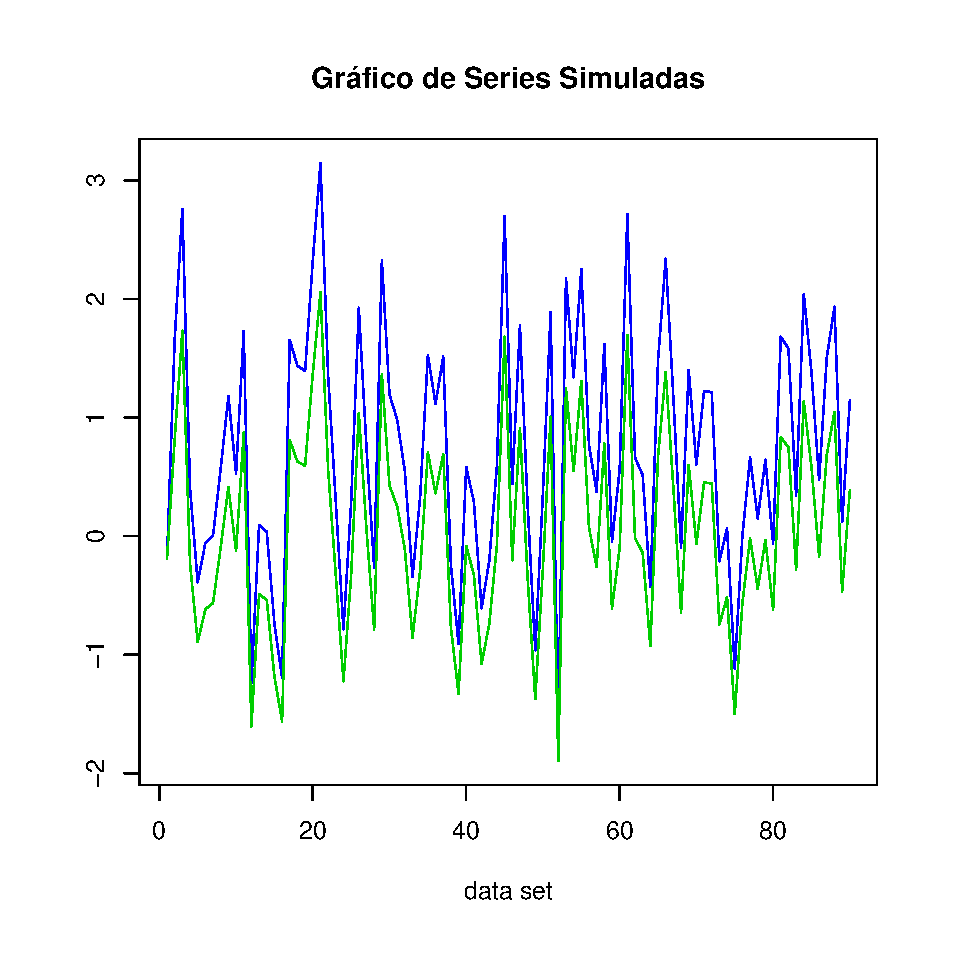
\includegraphics[height=5cm, width=6cm]{rho_1.ps}
  \caption{Valores de $\hat{\rho}_{X_{t},Y_{t}} \approx 1$.}
  \label{caja1}
\end{figure}

Cuando se habla del comportamiento de las series de tiempo, se est\'a en presencia de estructuras din\'amicas que no est\'an fijas, como en el caso de las variables aleatorias, ya que se ha calculado que grado de comovimiento tienen, entonces de acuerdo a su definici\'on un $\widehat{\rho}_{X_{t},Y_{t}}(h=1)$ cercano a 1, significa que las series se mueven juntas en cualquier per\'iodo de tiempo $[t_i,t_{i+1}]$.

\subsection{Anti comovimiento}
Estas series fueron simuladas para que el comovimiento entre las dos series este cercano a $-1$.

En el siguiente gr\'afico se puede apreciar un anti comovimiento, es decir, que sus conjuntos de pares de pendientes son inversamente proporcionales.
\begin{figure}[htp]
\centering
  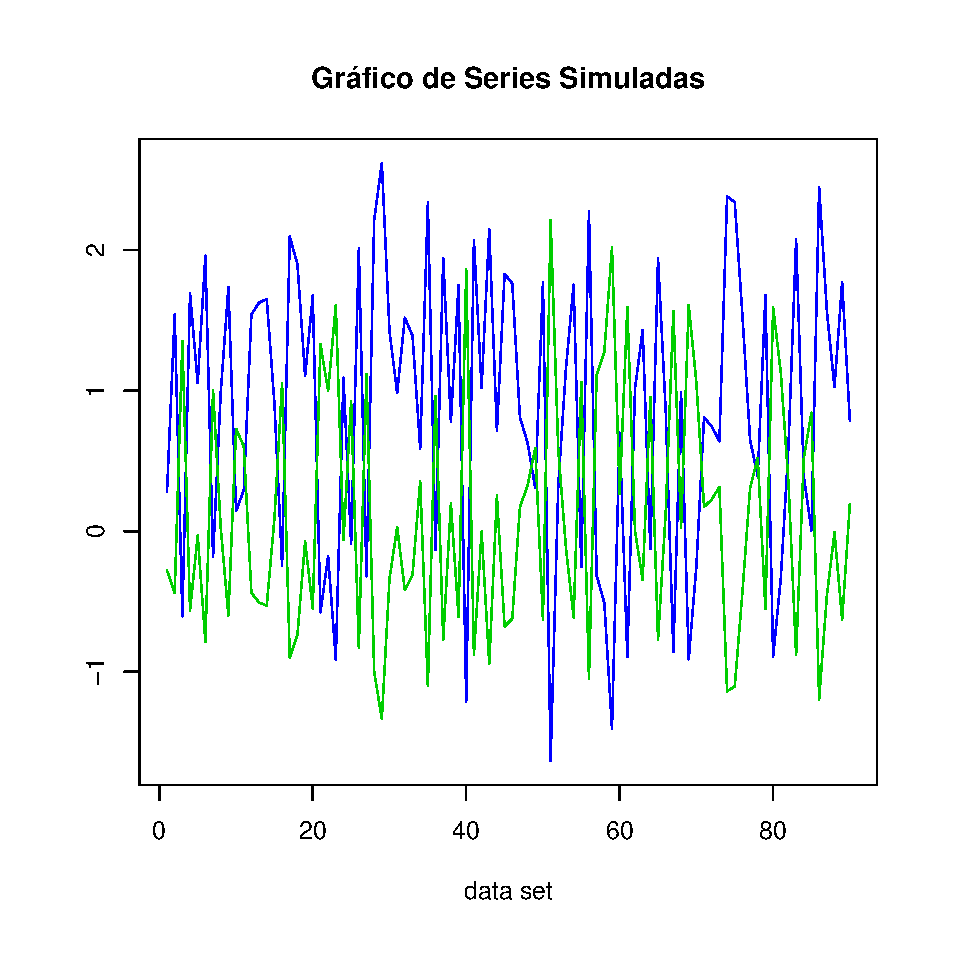
\includegraphics[height=5cm, width=6cm]{rho_-1.ps}
  \caption{Valores de $\hat{\rho}_{X_{t},Y_{t}} \approx -1$.}
  \label{caja2}
\end{figure}
Se puede ver como las series tienen un comportamiento inverso respecto del otro. Si calculamos su grado de comovimiento con el estimador muestral este es $-0.999$. Es decir, estas series comueven de manera inversa en cualquier periodo de tiempo $[t_i,t_{i+1}]$.

\subsection{Comovimiento nulo}
De igual forma, estas series fueron simuladas para que el comovimiento entre las dos series este cercano a $0$.

Finalmente, en este gr\'afico se puede observar que el conjunto de pares de pendientes no tiene nada en com\'un. Es decir, la series en cualquier p\'eriodo de tiempo no comueven. El \'Indice estimado es $0.0001$.

\begin{figure}[htp]
\centering
  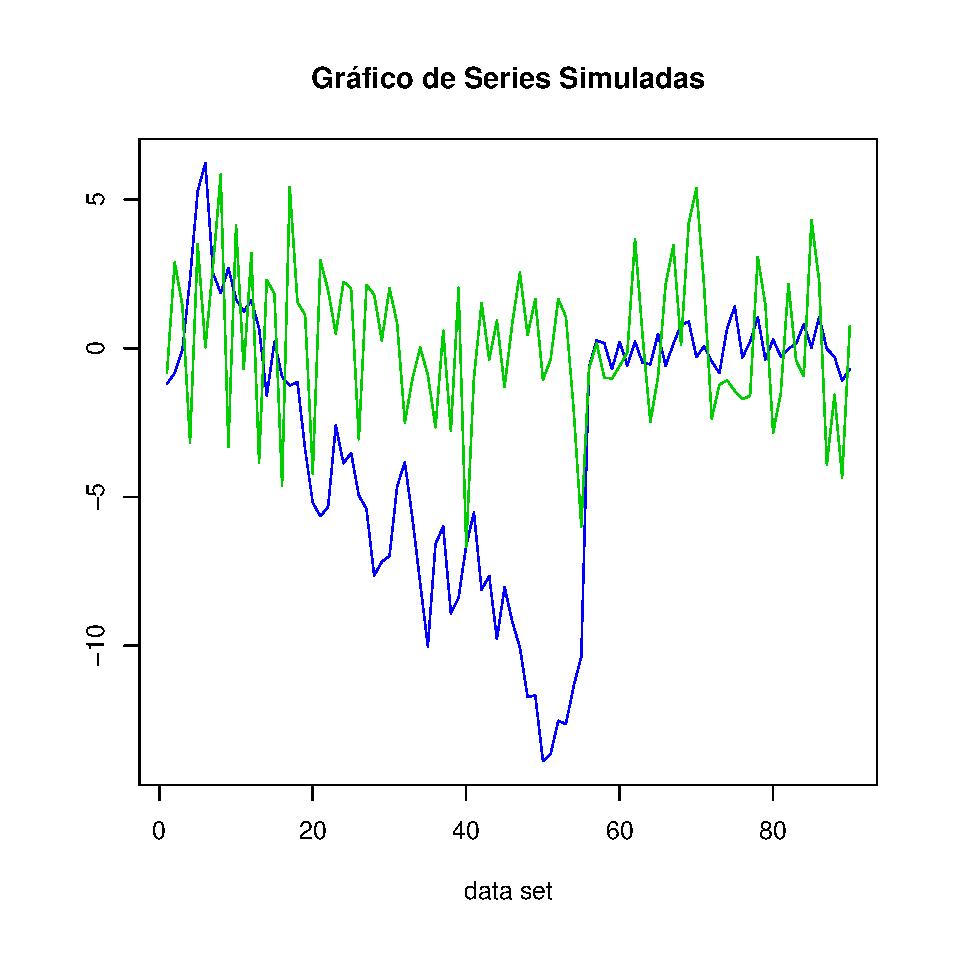
\includegraphics[height=5cm, width=6cm]{rho_0.eps}
   \caption{Valores de $\hat{\rho}_{X_{t},Y_{t}} \approx 0$.}
\label{caja3}
\end{figure}

\section{Propiedades}

Como ya se a dicho, las series de tiempo pueden ser modelados por procesos estoc\'asticos. Esta secci\'on se realizaron los siguientes c\'alculos para dos procesos lineales generales.

Ahora bien, para analizar la similaridad entre dos series de tiempo, se presentar\'an algunos c\'alculos que ser\'an asociados al \'Indice de Comovimiento. La importancia de esta secci\'on es presentar una medida de similaridad expl\'icita, expresada a trav\'es de dos modelos lineales generales. Tambi\'en, se discutir\'a la normalidad asint\'otica del Coeficiente de Codispersi\'on muestral. Entonces, sean dos procesos lineales generales de la forma:

\begin{eqnarray}
X_{t}&=&\sum_{j=0}^{\infty}\phi_{j}\epsilon_{1}(t-j),\\
Y_{t}&=&\sum_{k=0}^{\infty}\theta_{k}\epsilon_{2}(t-k),
\end{eqnarray}

tal que $\sum_{j=0}^{\infty}\phi_{j}< \infty$, $\sum_{k=0}^{\infty}\theta_{k} < \infty$ y $\epsilon_{1}$ y $\epsilon_{2}$ son ruidos blancos con media 0 y varianza $\sigma^{2}$ y $\tau^{2}$ respectivamente. Adem\'as, consideremos la estructura de covarianza para los errores dada por

\begin{eqnarray}
\mathbb Cov(\epsilon_{1}(t),\epsilon_{2}(s)) = \left\{
\begin{array}{cl}
\rho\tau\sigma&\mbox{si } t=s,\\
0&\mbox{en otro caso}.
\end{array}\right.
\end{eqnarray}

Hay varios procesos que satisfacen la forma lineal general, por
ejemplo para procesos autoregresivos de orden 1 y procesos de
media m\'ovil de orden 1. Sin embargo, para procesos ARMA de orden
superior no hay una forma expl\'icita (an\'alitica para $\rho_{X_{t},Y_{t}}(h)$).\\
Ahora se desarrollara los siguientes c\'alculos. Sea:
\begin{eqnarray*}
\mathbb E[X_{t+h}-X_{t}][Y_{t+h}-Y_{t}]&=&\mathbb E[X_{t+h}Y_{t+h}]-\mathbb E[X_{t+h}Y_{t}]-\mathbb E[X_{t}Y_{t+h}]+\mathbb E[X_{t}Y_{t}],
\end{eqnarray*}
\begin{eqnarray*}
\mathbb E[X_{t+h}Y_{t+h}]&=&\mathbb
E\left[\left(\sum_{j=0}^{\infty}{\phi_{j}\epsilon_{1}(t+h-j)}\right)\left(\sum_{k=0}^{\infty}{\theta_{k}\epsilon_{2}(t+h-k)}\right)\right],\\
&=&\sum_{j=0}^{\infty}{\sum_{k=0}^{\infty}{\phi_{j}\theta_{k}}\mathbb
E[\epsilon_{1}(t+h-j)\epsilon_{2}(t+h-k)]},\\
\end{eqnarray*}

Si $t+h-j=t+h-k$, entonces $j=k$. Por lo tanto

\begin{eqnarray*}
\mathbb E[X_{t+h}Y_{t+h}]&=&\sum_{j=0}^{\infty}{\phi_{j}\theta_{j}\rho\tau\sigma}.\\
\mathbb E[X_{t+h}Y_{t}]&=&\mathbb
E\left[\left(\sum_{j=0}^{\infty}{\phi_{j}\epsilon_{1}(t+h-j)}\right)\left(\sum_{k=0}^{\infty}{\theta_{k}\epsilon_{2}(t-k)}\right)\right]\\
&=&\sum_{j=0}^{\infty}{\sum_{k=0}^{\infty}{\phi_{j}\theta_{k}}\mathbb
E[\epsilon_{1}(t+h-j)\epsilon_{2}(t-k)]}
\end{eqnarray*}

Si $t+h-j=t-k$, entonces $j=k+h$. Luego

\begin{eqnarray*}
\mathbb E[X_{t+h}Y_{t}]&=&\sum_{j=0}^{\infty}{\phi_{k+h}\theta_{k}\rho\tau\sigma.}\\
\mbox{Adem\'as,   } \mathbb E[X_{t+h}Y_{t}]&=&\sum_{j=0}^{\infty}{\phi_{j+h}\theta_{j}\rho\tau\sigma.}\mbox{    Similarmente,  }\\
\mathbb E[X_{t}Y_{t+h}]&=&\mathbb
E\left[\left(\sum_{j=0}^{\infty}{\phi_{j}\epsilon_{1}(t-j)}\right)\left(\sum_{k=0}^{\infty}{\theta_{k}\epsilon_{2}(t+h-k)}\right)\right]\\
\end{eqnarray*}
\begin{eqnarray*}
&=&\sum_{j=0}^{\infty}{\sum_{k=0}^{\infty}{\phi_{j}\theta_{k}}\mathbb
E[\epsilon_{1}(t-j)\epsilon_{2}(t+h-k)]}\\
\mbox{Si $t-j=t+h-k$, entonces $k=j+h$}\\
\mathbb E[X_{t}Y_{t+h}]&=&\sum_{j=0}^{\infty}{\phi_{j}\theta_{j+h}\rho\tau\sigma.}\mbox{  Finalmente,  }\\
\mathbb E[X_{t}Y_{t}]&=&\mathbb
E\left[\left(\sum_{j=0}^{\infty}{\phi_{j}\epsilon_{1}(t-j)}\right)\left(\sum_{k=0}^{\infty}{\theta_{k}\epsilon_{2}(t-k)}\right)\right]\\
&=&\sum_{j=0}^{\infty}{\sum_{k=0}^{\infty}{\phi_{j}\theta_{k}}\mathbb
E[\epsilon_{1}(t-j)\epsilon_{2}(t-k)]}\\
\mbox{Si $t-j=t-k$, entonces $k=j$. Por lo tanto, }\\
\mathbb E[X_{t}Y_{t}]&=&\sum_{j=0}^{\infty}{\phi_{j}\theta_{j}\rho\tau\sigma}\\
\mbox{Note que $\mathbb E[X_{t+h}Y_{t+h}]=\mathbb E[X_{t}Y_{t}]$}
\end{eqnarray*}

Para el c\'alculo del denominador del coeficiente se tiene que

\begin{eqnarray*}
\mathbb E[X_{t+h}-X_{t}]^{2}&=&\mathbb Var[X_{t+h}-X_{t}]=\mathbb Var[X_{t+h}]+\mathbb Var[X_{t}]-2\mathbb Cov[X_{t+h}X_{t}].\\
\mathbb Var[X_{t+h}]&=&\mathbb Var\left[\sum_{j=0}^{\infty}\phi_{j}\epsilon_{1}(t+h-j)\right]=\sum_{j=0}^{\infty}\phi_{j}^{2}\mathbb Var[\epsilon_{1}(t+h-j)]=\sum_{j=0}^{\infty}\phi_{j}^{2}\sigma^{2}.\\
\mathbb Var[X_{t}]&=&\mathbb Var\left[\sum_{j=0}^{\infty}\phi_{j}\epsilon_{1}(t-j)\right]=\sum_{j=0}^{\infty}\phi_{j}^{2}\mathbb E[\epsilon_{1}(t-j)]=\sum_{j=0}^{\infty}\phi_{j}^{2}\sigma^{2}.\\
\mathbb Cov[X_{t+h}X_{t}]&=&\mathbb E[X_{t+h}X_{t}]-\mathbb E[X_{t+h}]\mathbb E[X_{t}]=\mathbb E[X_{t+h}X_{t}]\\
\mathbb E[X_{t+h}X_{t}]&=&\mathbb E\left[\left(\sum_{j=0}^{\infty}{\phi_{j}\epsilon_{1}(t+h-j)}\right)\left(\sum_{k=0}^{\infty}{\phi_{k}\epsilon_{1}(t-k)}\right)\right]\\
&=&\sum_{j=0}^{\infty}{\sum_{k=0}^{\infty}{\phi_{j}\phi_{k}}\mathbb
E[\epsilon_{1}(t+h-j)\epsilon_{1}(t-k)]}
\end{eqnarray*}
Si $t+h-j=t-k$, entonces, $k=j+h$
\begin{eqnarray*}
&=&\sum_{j=0}^{\infty}\phi_{j}\phi_{j+h}\sigma^{2}
\end{eqnarray*}
Similarmente, se tiene:
\begin{eqnarray*}
\mathbb E[Y_{t+h}-Y_{t}]^{2}&=&\mathbb Var[Y_{t+h}-Y_{t}]=\mathbb Var[Y_{t+h}]+\mathbb Var[Y_{t}]-2\mathbb
Cov[Y_{t+h}Y_{t}]\\
\mathbb Var[Y_{t+h}]&=&\mathbb Var\left[\sum_{k=0}^{\infty}\theta_{k}\epsilon_{2}(t+h-k)\right]=\sum_{k=0}^{\infty}\theta_{k}^{2}\mathbb Var[\epsilon_{2}(t+h-k)]=\sum_{k=0}^{\infty}\theta_{k}^{2}\tau^{2}.\\
\end{eqnarray*}
\begin{eqnarray*}
\mathbb Var[Y_{t}]&=&\mathbb Var\left[\sum_{k=0}^{\infty}\theta_{k}\epsilon_{2}(t-k)\right]=\sum_{j=0}^{\infty}\theta_{k}^{2}\mathbb Var[\epsilon_{2}(t-k)]=\sum_{k=0}^{\infty}\theta_{k}^{2}\tau^{2}.\\
\mathbb Cov[Y_{t+h}Y_{t}]&=&\mathbb E[Y_{t+h}Y_{t}]-\mathbb E[Y_{t+h}]\mathbb E[Y_{t}]=\mathbb E[Y_{t+h}Y_{t}]\\
\mathbb E[Y_{t+h}Y_{t}]&=&\mathbb E\left[\left(\sum_{j=0}^{\infty}{\theta_{j}\epsilon_{2}(t+h-j)}\right)\left(\sum_{k=0}^{\infty}{\theta_{k}\epsilon_{2}(t-k)}\right)\right]\\
&=&\sum_{j=0}^{\infty}{\sum_{k=0}^{\infty}{\theta_{j}\theta_{k}}\mathbb
E[\epsilon_{1}(t+h-j)\epsilon_{1}(t-k)]}
\end{eqnarray*}
Si $t+h-j=t-k$, entonces, $k=j+h$
\begin{eqnarray*}
\mathbb E[Y_{t+h}Y_{t}]&=&\sum_{j=0}^{\infty}\theta_{k}\theta_{k+h}\tau^{2}
\end{eqnarray*}

Ahora si juntamos los t\'erminos y factorizamos nos queda.
\begin{eqnarray*}
\rho_{X_t,Y_t}(h)&=&\rho\cdot\frac{\sum_{j=0}^{\infty}(2\phi_{j}\theta_{j}-\phi_{j+h}\theta_{j}-\phi_{j}\theta_{j+h})}{2\sqrt{\sum_{j=0}^{\infty}(\phi_{j}^{2}-\phi_{j}\phi_{j+h})\sum_{j=0}^{\infty}(\theta_{j}^{2}-\theta_{j}\theta_{j+h})}}.
\end{eqnarray*}

Como caso particular:\\
Cuando ${X_{t}}$ $\sim$ AR(1) y ${Y_{t}}$ $\sim$ AR(1), los param\'etros $\phi$ y $\theta$ satisfacen $\phi_{j}=\phi^{j}$ ,$|\phi|<1$ y $\theta_{j}=\theta^{j}$, $|\theta|<1$,$|\theta\phi|<1$

Usando las siguientes identidades.
\begin{eqnarray*}
\sum_{k=0}^{\infty}{\theta^{k}\phi^{k}}=\sum_{k=0}^{\infty}{(\theta\phi)^{k}}&=&\frac{1}{1-\theta\phi},\\
\sum_{k=0}^{\infty}{\theta^{k}\phi^{k+h}}=\phi^{h}\sum_{k=0}^{\infty}{(\theta\phi)^{k}}&=&\frac{\phi^{h}}{1-\theta\phi},\\
\sum_{k=0}^{\infty}{\theta^{k}\phi^{k+h}}=\phi^{h}\sum_{k=0}^{\infty}{(\theta\phi)^{k}}&=&\frac{\phi^{h}}{1-\theta\phi},\\
\sum_{k=0}^{\infty}{\phi^{2k}}&=&\frac{1}{1-\phi^{2}},\\
\sum_{k=0}^{\infty}{\theta^{2k}}&=&\frac{1}{1-\theta^{2}},\\
\sum_{k=0}^{\infty}{\phi^{k}\phi^{k+h}}=\phi^{h}\sum_{k=0}^{\infty}{(\phi)^{2k}}&=&\frac{\phi^{h}}{1-\phi^{2}},\\
\sum_{k=0}^{\infty}{\theta^{k}\theta^{k+h}}=\phi^{h}\sum_{k=0}^{\infty}{(\theta)^{2k}}&=&\frac{\phi^{h}}{1-\theta^{2}},
\end{eqnarray*}
Se tiene
\begin{eqnarray}
\rho_{X_t,Y_t}(h=1)&=&\rho\cdot\frac{(2-\phi-\theta)\sqrt{(1+\phi)(1+\theta)}}{1-\phi\theta}.
\end{eqnarray}
Desde aqu\'i se puede apreciar una forma expl\'icita del Coeficiente de Codispersi\'on $\rho_{X_t,Y_t}(h=1)$. El Coeficiente de Codispersi\'on es una versi\'on corregida del coeficiente de correlaci\'on cl\'asico. Este resultado fue obtenido por Rukhin y Vallejos (2008). Las propiedades asint\'oticas de  $\widehat{\rho}(h)$ fueron establecidas para el proceso $\mathbb Z_{s}=(\mathbb X_{s},\mathbb Y_{s})^{t}$ admitiendo la siguiente estructura,
\begin{eqnarray}
\mathbb Z_{s+h}-\mathbb Z_{s}=\sum_{l}\mathbb A_{l}\epsilon_{s-l},
\end{eqnarray}
Donde $\mathbb A_{l}=\mathbb A_{h}(l)$ son matrices $2 \times 2$ definida para todo $l$ tal que, $\sum\|\mathbb A(l)\|^{2}<\infty$, donde $\|\cdot\|$ denota cualquier norma matricial y $\epsilon_{t}$ son vectores independientes con media cero y matriz de covarianza $\Sigma$.

\begin{thm}{\rm
  Si el valor observado admite la representaci\'on del proceso $Z_{t}=(X_{t},Y_{t})^{t}$ (1.8.5) con matrices
  $A(k,l)=diag(\alpha_{kl},\beta_{kl})$, la distribuci\'on limite
  de $M[\hat{\rho_{X,Y}(h)-\rho}]$ es normalmente distribu\'ida con media 0 y
  varianza
  \begin{eqnarray}
  \nu^{2}&=&\left(1-\frac{\rho^{2}\sum_{s=0}^{\infty}{(\alpha_{s}\beta_{s})^{2}}}{\sum_{s=0}^{\infty}{\alpha_{s}^{2}}\sum_{s=0}^{\infty}{\beta_{s}^{2}}}\right).
  \end{eqnarray}
}
\end{thm}
Con este resultado, se han realizados trabajos con D\'ocimas de hip\'otesis, intervalos de Confianza y Bandas de confianzas para el Coeficiente de Codispersi\'on (Ver Rukhin y Vallejos, 2008).

La ventaja de encontrar una forma expl\'icita para la varianza del coeficiente facilita los c\'alculos para d\'ocimar y encontrar intervalos de Confianza ya que en caso contrario, habr\'ia que calcular la varianza, a trav\'es, de m\'etodos de re-muestreo.

\section{Limitaciones te\'oricas}

Dentro de las limitaciones te\'oricas se puede mencionar que para modelos con muchos pa\-r\'a\-me\-tros no existe una forma anal\'itica para el coeficiente, en este caso es necesario implementar t\'ecnicas computacionales. Cabe,
mencionar que para series de tiempo no estacionarias el \'indice de codispersi\'on no ha sido estudiado. Cuando una de las series presenta outliers, el coeficiente de codispersi\'on es muy sensible. La definici\'on de una version robusta del coeficiente de Codispersi\'on a\'un es un problema abierto.

\section{M\'etodos no par\'ametricos}

En la literatura existe una medida de asociac\'ion para procesos espaciales. Tj$\phi$stheim (1978), propone una medida de asociaci\'on para variables espaciales, esta medida est\'a basada en los rangos de las observaciones y la localizaci\'on de las coordenadas de los puntos medios. 
\def\baselinestretch{1}
\chapter{Agrupamiento de series temporales}
\def\baselinestretch{1.0}
\goodbreak
%%%------------Introduccion---------------------------------------
\section{Introducci\'on}
En este Cap\'itulo se dar\'a una definici\'on del \'Indice de Disimilaridad, para as\'i implementar una medida con el cual se trabajar\'a para la
clasificaci\'on de series temporales.

La motivaci\'on de analizar el comportamiento de un par de series temporales, es mayor a\'un cuando \'este se extiende para un conjunto de series temporales.

Ahora bien, como s\'imil al an\'alisis de cluster, es necesario extender algunos m\'etodos ya conocidos de agrupaci\'on, para un conjunto de variables aleatorias a trav\'es del tiempo. La variaci\'on de esta t\'ecnica, es considerar la informaci\'on del comovimiento a trav\'es del tiempo de los distintos pares de series temporales, donde el an\'alisis multivariante cl\'asico no considera.

El an\'alisis por agrupaci\'on (Cluster analysis) es una t\'ecnica
muy utilizada en problemas multivariados donde se quiere agrupar
unidades experimentales con ciertas caracter\'isticas o
generalizar grupo de variables de inter\'es. El objetivo
de este Cap\'itulo es definir algunas t\'ecnicas de
agrupaci\'on. Las t\'ecnicas m\'as usadas en este contexto son:

\begin{enumerate}
  \item M\'etodos de agrupaci\'on no jer\'arquicos.
  \item M\'etodos de agrupaci\'on jer\'arquicos.
\end{enumerate}
Estas definiciones ayudar\'an de base para definir una nueva medida de proximidad entre series temporales, asociados a las t\'ecnicas cl\'asicas de agrupaci\'on.
\section{M\'etodos de Agrupaci\'on}
Dependiendo del m\'etodo de agrupaci\'on que utilicemos los resultados finales variar\'an. Entonces, cada m\'etodo tiene una caracter\'istica en particular que es necesario considerar, en esta secci\'on se estudiar\'an los siguientes m\'etodos de agrupaci\'on:
\begin{enumerate}
  \item \textbf{M\'etodos de agrupaci\'on no jer\'arquicos}
   Se usan para agrupar objetos en un conjunto de k-cluster
  predeterminados, se parte de un conjunto inicial de clusters
  elegidos al azar luego se van cambiando de modo iterativo, habitualmente se usa el m\'etodo de las k-medias.
  \\\textbf{M\'etodo de las k-medias}
  \\Es un m\'etodo que permite asignar a cada observaci\'on el cluster
  que se encuentra m\'as pr\'oximo en t\'erminos el centroide (Valor medio de las observaciones de las variables en el valor del
  conglomerado).
  \begin{itemize}
  \item Se eligen al azar k-clusters iniciales.
  \item Para el conjunto de observaciones se vuelve a calcular la
  distancia al centroide de los clusters y se reasignan a los que
  est\'an mas pr\'oximos. Se vuelven a calcular los centroides de los
  k-cluster despu\'es de las reasignaciones de los elementos.
  \item Se repiten los pasos anteriores hasta que no se produzca
  ninguna reasignaci\'on.
  \end{itemize}
  \item \textbf{M\'etodos de agrupaci\'on jer\'arquicos}
  \\\textbf{M\'etodos Divisivos}
  \\Se comienza con un gran conglomerado que contiene todas las
  observaciones u objetos en los pasos sucesivos en las
  observaciones que son m\'as diferentes, se dividen y se construyen
  conglomerados m\'as peque\~{n}os. Este proceso continua hasta que cada
  observaci\'on es un mismo conglomerado.
  \\\textbf{2.1 M\'etodo de encadenamiento simple (Vecino m\'as cercano)}
  \\ Se basa en la distancia m\'inima, encuentra los dos objetos
  separados por la distancia m\'as peque\~na y las coloca en el primer
  conglomerado, a continuaci\'on se encuentra la distancia m\'as peque\~na
  o bien un tercer objeto. Se une a los dos primeros para formar
  un conglomerado o se forma un nuevo conglomerado de dos miembros.
  El proceso continua hasta que todos los objetos se encuentren en un
  conglomerado.
  \\\textbf{2.2 M\'etodo de encadenamiento completo (Vecino m\'as lejano)}
  \\ Este m\'etodo es similar al interior escepto que el criterio de
  aglomeramiento se basa en la distancia m\'axima.
\end{enumerate}

Tambi\'en, el uso de dendogramas es una herramienta \'util cuando se quiere gr\'aficar grupos.

El m\'etodo que se utilizar\'a para clasificaci\'on es el de agrupaci\'on jer\'arquico, ya que, se asumir\'a que no se conocen la cantidad de grupos iniciales. En nuestro an\'alisis usaremos el software R.

\section{\'Indice de Disimilaridad Adaptativo}
Para la clasificaci\'on y agrupaci\'on de series temporales es necesario tener en cuenta la estructura de correlaci\'on temporal, tanto como su comportamiento respecto de su comovimiento a trav\'es del tiempo,  como el comportamiento respecto de su cercan\'ia entre las series. En esta secci\'on se presentar\'a una propuesta para abarcar dichos elementos en la agrupaci\'on de series temporales.

Existen autores que se han interesado en la agrupaci\'on de series temporales, por ejemplo Liao (2005) hace una rese\~na de t\'ecnicas, medidas y algoritmos para la clasificaci\'on de series temporales. Por otra parte, Chouakria y Nagabbhusham (2007) estudiaron un m\'etodo para detectar la interdependencia entre las series, dado que con medidas convencianales, no logran captar su dependencia temporal y proponen una medida alternativa que cubre estos dos aspectos del an\'alisis de series temporales. A continuaci\'on se har\'a una peque\~na descripci\'on de \'estos m\'etodos, introduciendo definiciones cl\'asicas de medidas de desemejanzas, entre ellas se pueden destacar.
\subsection{Distancia Euclidiana}
Sean $X_{t}=(x_1,\ldots,x_n)$ e $Y_{t}=(y_1,\ldots,y_n)$ dos
series de tiempo de $n$ valores observados en el tiempo en los
instantes $t_1,\ldots,t_n$. La distancia Euclidiana $\delta_{E}$
entre ${X_{t}}$ e ${Y_{t}}$ est\'a definida como:
\begin{eqnarray}
\delta_{E}&=&\sqrt{\sum_{i=1}^{n}(x_i-y_i)^2}.
\end{eqnarray}
\subsection{Distancia de Minkowski}
Para dos secuencias $X_t$ e $Y_t$ la distancia de Minkowski $\delta_M$ de orden $p$ entre $X_t$ e $Y_t$ est\'a definida como:
\begin{eqnarray}
\delta_{M}&=&\sqrt[p]{\sum_{i=1}^{n}|x_i-y_i|^{p}}.
\end{eqnarray}
\subsection{Distancia de Frech\'et}
Se define una rejilla $r \in M$ entre dos series de tiempo $X_{t}=(x_{1},x_{2},\ldots,x_{n})$ e $Y_{t}=(y_{1},y_{2},\ldots,y_{k})$ como la secuencia de pares preservando el orden de la informaci\'on.
\[r=\left((x_{a_1},y_{b_1}),(x_{a_2},y_{b_2}),\ldots,(x_{a_n},y_{b_m})\right)\]
con $a_{i}, i \in \{1,\ldots,n\}$,$b_{j}, j \in \{1,\ldots,m\}$ y satisfaciendo  para $i \in \{1,\ldots,m-1\}$ la siguiente condici\'on: $a_{1}=1$,$b_{m}=k$ $a_{i}=(a_{i}\mbox{   \'o   } a_{i+1})$ y $b_{j}=(b_{j}\mbox{  \'o     } b_{j+1})$.\\
Se define $|r|=\max_{i=1,\ldots,m}|x_{a_i}-y_{b_i}|$, la rejilla $|r|$ est\'a representada por la m\'axima distancia entre dos observaciones pareadas.\\
La distancia $\delta_{F}(X_{t},Y_{t})$ se define como:
\begin{eqnarray}
\delta_{F}(X_{t},Y_{t})&=&\min_{r \in M}|r|=\min_{r \in M}\left(\max_{i=1,\ldots,m}|x_{a_i}-y_{b_i}|\right)
\end{eqnarray}

\section{Alineamiento de tiempo distorsionado\\
 (Dynamic time warping DTW)}

El alineamiento de tiempo distorsionado (DTW) es una t\'ecnica que encuentra la alineaci\'on \'optima entre dos series temporales. El alineamiento de tiempo distorsionado es a menudo usado en el reconocimiento del lenguaje hablado para
determinar si dos formas de onda representan la de la misma forma de locuci\'on hablada.

El alineamiento de tiempo distorsionado ha sido \'util dentro de muchas otras disciplinas, la rob\'otica, la manufactura, y la medicina. Un ejemplo de c\'omo una serie temporal est\'a  distorsionada es mostrado en la siguiente figura.

\begin{figure}[!htp]
\centering
\fbox{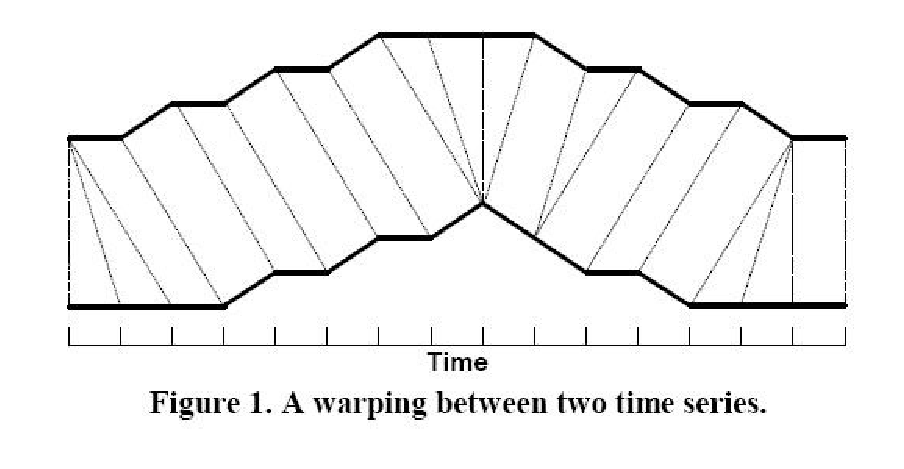
\includegraphics[height=4cm, width=5cm]{warping_two_series.eps}}
\caption{Alineamiento de tiempo distorsionado} \label{caja}
\end{figure}

En la Figura 2.1, cada l\'inea vertical conecta un punto en una serie temporal con su punto co\-rres\-pon\-dien\-te, similar en la otra serie temporal. Las l\'ineas realmente tienen valores similares en el eje vertical pero han sido separados, as\'i es que en las l\'ineas verticales entre ellos pueden ser miradas m\'as f\'acilmente.

Si ambas series temporales en la figura fueran id\'enticas, todas las l\'ineas ser\'ian l\'ineas directamente verticales porque todos los puntos ser\'ian similares entre ellos.

\subsection{Formulaci\'on del problema}
El problema del alineamiento de tiempo distorsionado es definido como sigue:

Dadas dos series de tiempo $X_{t}=(x_1,\ldots,x_{i},\ldots,x_m)$ e $Y_{t}=(y_1,\ldots,y_{j},\ldots,y_n)$ de largo $m$ y $n$ respectivamente. Se construye el camino distorsionado que llamaremos $W_{k}$, esta es una secuencia de pares de puntos ordenados, basado en los \'indices de las series $X_{t}$ e $Y_{t}$, donde:

$|r|=W_{k}=\{w_{1},\ldots,w_{K}\}$, $\max\{m,n\}\leq K\leq n\cdot m$. Adem\'as, $K=m \times n$ es la longitud m\'axima del camino distorsionado.
El camino distorsionado $W_{k}$ se define de la siguiente forma:

\begin{eqnarray}
w_{k}=(i,j), \mbox{    con $k=1,\ldots,K$}
\end{eqnarray}

donde $i$ es el \'indice de la Serie $X_t$ y $j$ es el \'indice de la serie $Y_t$.

El camino distorsionado debe empezar desde $w_{1}=(1,1)$ y el final de ambas en $w_K=(m,n)$. Esto asegura que cada \'indice de ambas serie temporales es usado en el camino distorsionado. Hay una restricci\'on en el camino distorsionado que obliga a $i$ y $j$ a ser monotonamente creciente.\\
Se define mas formalmente:

\[r=\left((x_{a_1},y_{b_1}),(x_{a_2},y_{b_2}),\ldots,(x_{a_m},y_{b_n})\right)=(w_{1},w_{2},\ldots,w_{K}),\]
con $a_{i}, i \in \{1,\ldots,n\}$,$b_{j}, j \in \{1,\ldots,n\}$ y satisfaciendo  para $i \in \{1,\ldots,m-1\}$ la siguiente condici\'on: $a_{1}=1$,$b_{n}=k$ $a_{i}=(a_{i}\mbox{   \'o   } a_{i+1})$ y $b_{j}=(b_{j}\mbox{  \'o     } b_{j+1})$.

Para detreminar DTW para dos secuencias de tiempo, construimos una matriz de $m\cdot n$ donde $(i^{th}, j^{th})$ son elementos de la matriz contiene la distancia $d(x_{a_i}, y_{b_i})$ entre los dos puntos $x_{a_i}$ e $y_{b_i}$, es decir,$d(x_{a_i}, y_{b_i})=|x_{a_i}-y_{b_i}|$. Cada elemento matricial $(i, j)$ corresponde a la alineaci\'on entre el punto de $x_{a_i}$ e $y_{b_i}$.

Este camino puede ser encontrado usando programaci\'on din\'amica para evaluar la siguiente recurrencia, que defina la distancia acumulativa $\gamma(i,j)$ como la distancia $d(i, j)$ encontrada en la celda actual y el m\'inimo de las distancias acumulativas de los elementos adyacentes,

\begin{eqnarray}
\gamma(i,j)&=&d(i,j)+min\{\gamma(i-1,j-1),\gamma(i-1,j),\gamma(i,j-1)\}.
\end{eqnarray}

\subsection{Hacia el Alineamiento de tiempo distorsionado}

El Alineamiento de tiempo distorsionado es un algoritmo para medir la similitud entre dos secuencias que pueden variar en el tiempo o en la velocidad. DTW se ha aplicado en video, audio y gr\'aficos, de hecho en cualquier dato que pueda ser convertido en una representaci\'on lineal se puede analizar con DTW.  Una conocida ha sido la aplicaci\'on autom\'atica de reconocimiento de voz, para hacer frente a diferentes velocidades haciendo uso de la palabra.

En general, DTW es un m\'etodo que permite a un ordenador encontrar una \'optima adecuaci\'on entre dos secuencias dadas (por ejemplo, series de tiempo), con ciertas restricciones.

Un ejemplo de las restricciones impuestas a la adecuaci\'on de las secuencias se encuentra en la monotocidad de la cartograf\'ia en la dimensi\'on temporal.  La continuidad es menos importante en DTW que en otros algoritmos de Coincidencia de patrones; DTW es un algoritmo especialmente adecuado para las secuencias de concordancia con la informaci\'on que falta.El proceso de optimizaci\'on se realiza utilizando programaci�n din\'amica, de ah\'i el nombre. Ejemplo de una de las muchas formas del algoritmo.
\begin{verbatim}
###############################################################################
#### RUTINA PARA DETERMINAR EL CAMINO DISTROSIONADO ###########################
  int DTWDistance (char s [1 .. n], char t [1 .. m], int d [1 .. n, 1 .. m]) (
      DTW declarar int [0 .. n, 0 .. m]
      declarar int i, j, el costo

      for i: = 1 to m
          DTW [0, i]: = infinito
      for i: = 1 hasta n
          DTW [i, 0]: = infinito
      DTW [0,0]: = 0

      for i: = 1 hasta n
          for j: = 1 to m
              coste: = d [s [i], t [j]]
              DTW [i, j]: = + costo m�nimo (DTW [i-1, j], / / inserci�n
                                         DTW [i, j-1], / / supresi�n
                                         DTW [i-1, j-1]) / / partido

      DTW retorno [n, m]
  )
##############################################################################
\end{verbatim}

Este algoritmo c\'alcula la distancia DTW para dos secuencias, donde los vectores pueden ser de distinto tama\~no. En la siguiente figura se puede apreciar que el algoritmo encuentra el camino mas corto entre dos series, que dependen de la similitud entre las mismas.

\begin{figure}[!htp]
\centering
\fbox{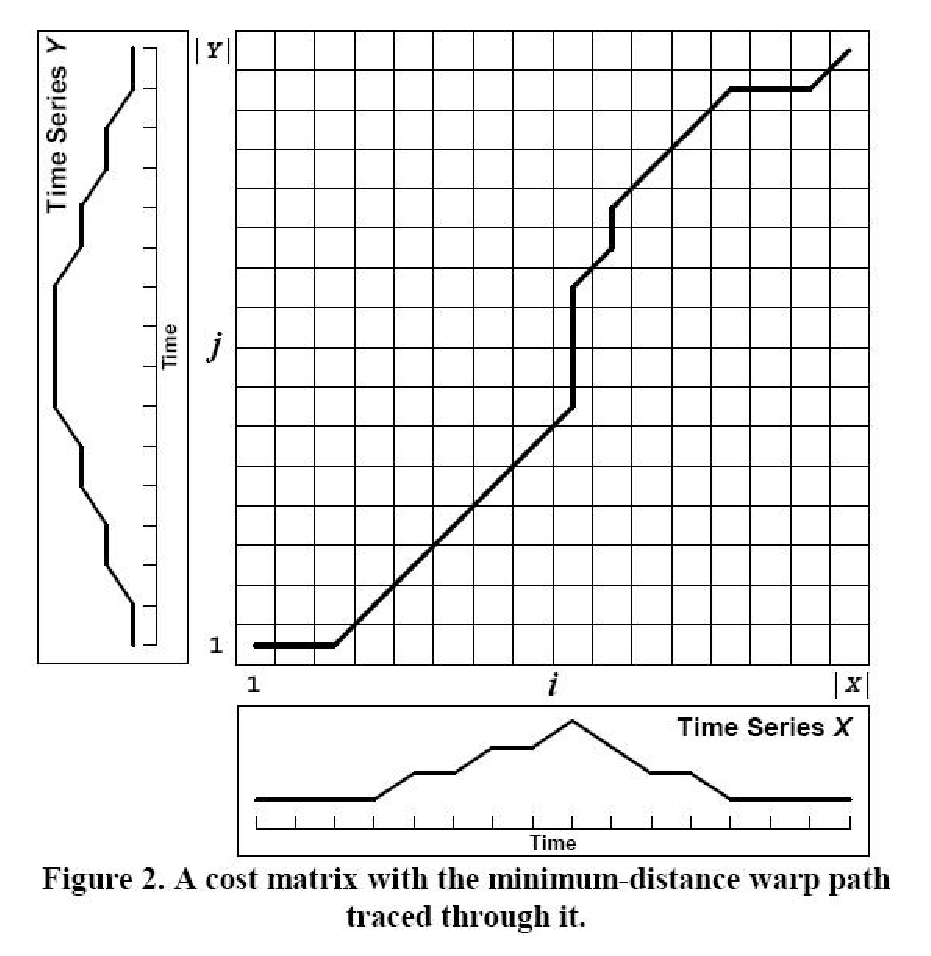
\includegraphics[height=4cm, width=5cm]{cost_minimun_distance.eps}}
\caption{Camino distorsionado} \label{caja}
\end{figure}

Ya mencionadas las caracter\'isticas se definir\'a mas formalmente la Distancia DTW.

\subsection{Definici\'on DTW}
Considere una nueva definici\'on de la rejilla propuesta en (2.3.3) como la suma de las distancias de todas las observaciones apareadas.
\begin{eqnarray}
|r|&=&\sum_{i=1}^{m}|x_{a_i}-y_{b_i}|.
\end{eqnarray}
Entonces la distancia $\delta_{DTW}$ se define de la siguiente manera:
\begin{eqnarray}
\delta_{DTW}(X_{t},Y_{t})&=&\min|r|=\min_{r\in M}\left(\sum_{i=1}^{m}|x_{a_i}-y_{b_i}|\right).
\end{eqnarray}

\subsection{Ejemplo}
La finalidad de este ejemplo es resumir esta secci\'on para dejar m\'as claro cuales son las bondades de DTW. Entonces, considere dos secuencias de tiempo. Sea $X_{t}=(1,0.34,0.65,2,3,3.4,1,1.2,0.88,5.9,7)$ e $Y_{t}=(2,5.5,5.67,3.45,7,3.3,2.43,1.34)$. Calcular $\delta_{DTW}(X_{t},Y_{t})$. Considere la siguiente rutina.

\begin{verbatim}
###############################################################################

library(dtw)
x<-c(1,0.34,0.65,2,3,3.4,1,1.2,0.88,5.9,7)
y<-c(2,5.5,5.67,3.45,7,3.3,2.43,1.34)
a<-dtw(x,y)
b<-a$distance
plot(a,xlab="indice de x",ylab="indice de y",main="Camino Distorcionado")
> length(x)
[1] 11
> length(y)
[1] 8
> b
[1] 26.45

#############################################################################
\end{verbatim}
En la salida de esta rutina se puede apreciar que la longitud del vector $X_{t}$ es de 11 elementos y la longitud del vector $Y_{t}$ es 8 elementos. Por otra parte la distancia es 26.45.\\
La opci\'on $\verb"plot(a)"$ en R muestra el siguiente gr\'afico.

\newpage
\begin{figure}[!htp]
\centering
\fbox{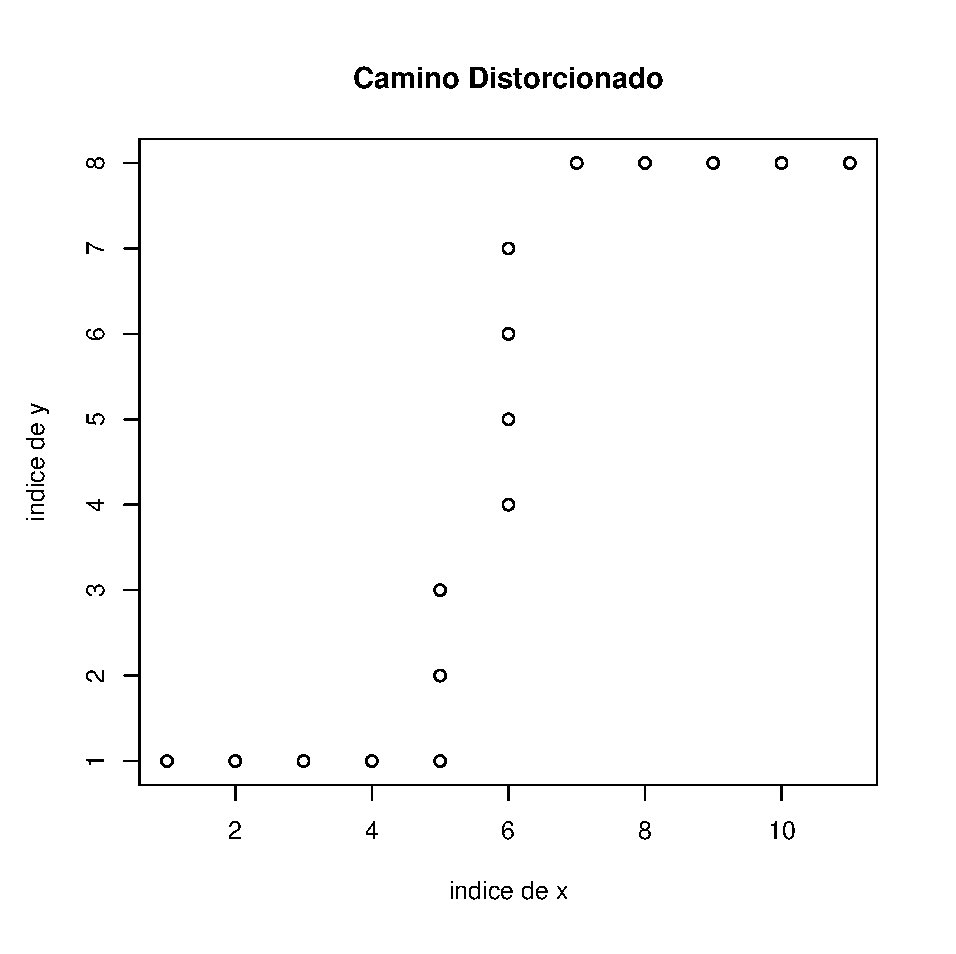
\includegraphics[height=5cm, width=7cm]{c_dtw.eps}}
\caption{Camino distorsionado de $\delta_{DTW}(X_{t},Y_{t})$.} \label{caja}
\end{figure}

Una de las caracter\'istica de DTW, es la representaci\'on gr\'afica de la similitud entre dos series temporales y en este caso se puede apreciar que las series no presentan un gran grado de similitud, ya que estos puntos no definen una linea recta.

Desde aqu\'i, se puede apreciar y entender m\'as f\'acilmente la definici\'on de camino distorsionado.

En esta secci\'on se han presentado las distancias $\delta_{E}$, $\delta_{M}$, $\delta_{F}$, y $\delta_{DTW}$ pero ellas ignoran la estructura temporal de los valores como proximidad, ya que, est\'an basada sobre las diferencias entre los valores $|x_{a_i}-y_{b_i}|$.

En la siguiente secci\'on se propondr\'a un \'Indice que considere la estructura de comovimiento y la cercan\'ia entre las series en el contexto de clasificaci\'on de series temporales.

\section{\'Indice de Disimilaridad Adaptativo para medidas de pro\-xi\-mi\-dad entre series de tiempo.}

Las medidas convencionales de proximidad en series temporales, est\'an basadas sobre la cercan\'ia de los valores observados de
las series de tiempo.

La idea de est\'a secci\'on es presentar un \'Indice  de Disimilaridad, que contenga la informaci\'on de la codipersi\'on o comovimiento y la cercan\'ia de las series temporales. En otras palabras se define la disimilaridad entre dos series de tiempo, considerando estas dos caracter\'isticas, uno el comportamiento respecto a su comovimiento y la otra sobre su cercan\'ia. Generalmente, se asume que esta medida entre las secuencias $X_t$ e $Y_t$ toman valores positivos.

Uno puede cuantificar el concepto de similaridad considerando el cl\'asico coeficiente de co\-rre\-la\-ci\'on de Pearson. Sin embargo, esta correlaci\'on gu\'ia una sobre estimaci\'on de la Codispersi\'on. De igual forma, el coeficiente de correlaci\'on de Spearman es tambi\'en usado como una medida de similaridad. No obstante, se ha visto que la correlaci\'on est\'a principalmente basada sobre los rangos y no sobre los  valores observados. Dejando de lado la informaci\'on respecto a su comovimiento.

\subsection{Correlaci\'on temporal para medidas de proximidad}
Ya se ha mencionado las desventajas de las medidas de distancias convencionales y los coeficientes de similaridad que no ayudan a establecer un \'indice que pueda conjugar estas dos ca\-rac\-te\-r\'is\-ti\-cas. Una estructura que considere la interdependencias entre dos serie puede deducirse considerando los siguientes elementos:

Sea $X_{t}=(x_1,\ldots,x_n)$ una colecci\'on de $n$ n\'umeros reales
independientes. La varianza cl\'asica de $X_{t}$ puede ser escrita en dos
vias equivalentes,
\begin{eqnarray}
Var(X_{t})=\frac{1}{n-1}{\sum_{i=1}^{n}(x_{i}-m)^2}=\frac{1}{n-1}{\sum_{i,i'}(x_i-m)^2},
\end{eqnarray}
donde $m$ es la media de los valores de $X_{t}$. Similarmente el coeficiente cl\'asico de correlaci\'on entre
$X_{t}=(x_1,\ldots,x_n)$ e $Y_{t}=(y_1,\ldots,y_n)$ puede ser escrito de dos formas:
\begin{eqnarray}
Corr_{X_{t},Y_{t}}=\frac{\sum_{i=i}^{n}(x_i-m_1)(y_i-m_2)}{\sqrt{Var({X_{t}})Var({Y_{t}})}}=\frac{\sum_{i,i'}(x_i-x_{i'})(y_i-y_{i'})}{\sqrt{\sum_{i,i'}(x_i-x_{i'})^{2}\sum_{i,i'}(y_i-y_{i'})^{2}}}.
\end{eqnarray}
En el caso general de medidas independientes varianza$/$covarianza y coeficiente de correlaci\'on son medidas basadas sobre la
contribuci\'on de todos los pares de medici\'on. A la inversa en el caso de las interdependencias se define una relaci\'on entre
vecino m\'as cercano.

La expresi\'on de la varianza puede ser descompuesta como sigue:
\begin{center}
\begin{eqnarray}
Var(X_{t})&=&\frac{1}{2n-1}{\sum_{i,i'}(x_i-x_{i'})^2}.
\end{eqnarray}
\end{center}

De igual forma,

\begin{eqnarray}
Var(S)&=&\frac{1}{2n-1}{\sum_{\mbox{$i$ es vecino de $i'$}}(x_i-x_{i'})^2}+\frac{1}{2n-1}{\sum_{\mbox{$i$ no es vecino de $i'$}}(x_i-x_{i'})^2}.
\end{eqnarray}

La idea principal para incluir la informaci\'on sobre la dependencia de las series, es una restricci\'on a la expresi\'on de la varianza$/$covarianza de los pares de valores dependientes (Vecinos).

\begin{eqnarray}
VarT(X_{t})=\frac{1}{2n-1}{\sum_{\mbox{$i$ no es vecino de $i'$}}(x_{i}-x_{i'})^2},
\end{eqnarray}

Para la similaridad, se considerara una relaci\'on temporal de
vecinos de orden $h$, medidas en el p\'eriodo ${[t_i,t_{i+h}]}$. Este coeficiente de
correlaci\'on temporal es definido como:

\begin{eqnarray}
\widehat{\rho}_{X_{t},Y_{t}}(h)=\frac{\sum_{i=i}^{n-1}(x_{i+h}-x_i)(y_{i+h}-y_{i})}{\sqrt{\sum_{i=1}^{n-1}(x_{i+h}-x_i)^{2}\sum_{i=i}^{n-1}(y_{i+h}-y_{i})^{2}}}.
\end{eqnarray}

donde $\widehat{\rho}_{X_{t},Y_{t}}(h)$ pertenece al intervalo $[-1,1]$. La interpretaci\'on de los valores se discuti\'o  en la secci\'on de ejemplos en el cap\'itulo I.

\subsection{\'Indice de Disimilaridad Adaptativo entre series de tiempo}

El prop\'osito de este cap\'itulo es apuntar a un nuevo \'Indice con aspiraci\'on a cubrir ambas medidas convencionales de similaridad y cercan\'ia
para la proximidad de valores y la correlaci\'on temporal entre dos series temporales para medir el comportamiento conjunto.


El resultado de la medida de disimilaridad debe tambi\'en permitir ajustar el peso de la contribuci\'on entre ambos cuantiles (Comovimiento y Cercan\'ia). Para ajustar el peso de la contribuci\'on de los cuantiles es necesario tener una funci\'on  $f(x)$ que module la distancia incrementando o dis\-mi\-nu\-yen\-do las medidas convencionales antes definidas.


Conforme con las especificaciones anteriores, se propone un \'Indice de Disimilaridad $D(X_{t},Y_{t})$ basado sobre una funci\'on de afinaci\'on autom\'atica que module el comportamiento de las medidas convencionales.


Ahora bien, en el contexto de an\'alisis de grupos (Cluster) Chouakria y  Na\-ga\-bhu\-shan (2007) propusieron un \'Indice de Disimilaridad Adaptativo para medidas de proximidad en series temporales, como una nueva medida de distancia, la cual definieron de la siguiente forma,

\begin{eqnarray}
D({X_{t}},{Y_{t}})&=&f(\widehat{\rho}_{X_{t},Y_{t}}(h))\delta_{C}({X_{t}},{Y_{t}}),
\end{eqnarray}

donde $f(x)$ es una funci\'on de afinaci\'on exponencial adaptativa, es dado por

\begin{eqnarray}
 f(x)&=&\frac{2}{1+exp(kx)},\mbox{  $k \geq 0$}.
\end{eqnarray}

y $\delta_{C}({X_{t}},{Y_{t}})$ es cualquier distancia convencional entre ${X_{t}}$ e ${Y_{t}}$. Note que la funci\'on $f(x)$ depende del estimador muestral del Coeficiente de Codispersi\'on. En la Figura 2.4, se puede apreciar la funci\'on de afinamiento adaptativo para distintos valores de $k$.

\begin{figure}[!htp]
\centering
\fbox{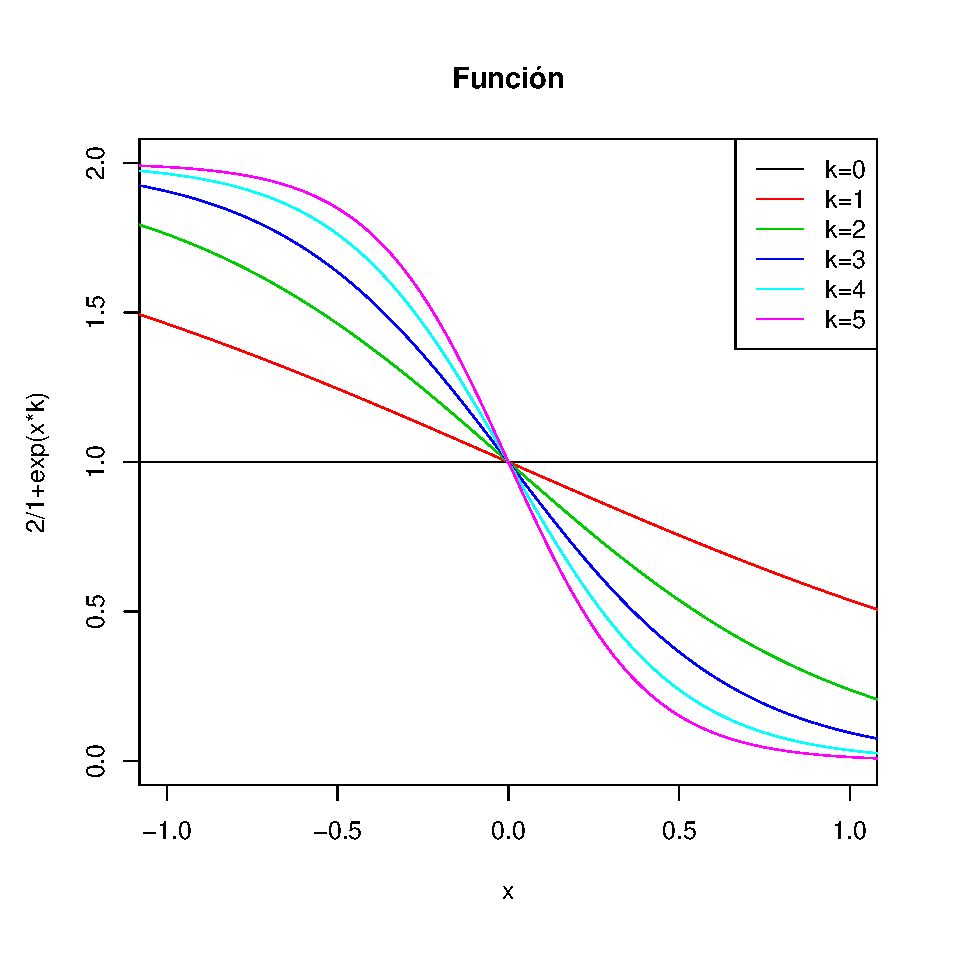
\includegraphics[height=5cm, width=6cm]{fat.eps}}
\caption{Funci\'on exponencial adaptativo} \label{caja}
\end{figure}
\newpage
La funci\'on de $k$ es modular con m\'as o menos fuerza la contribuci\'on de los cuantiles sobre las medidas convencionales. Esto se puede apreciar en la tabla.

\begin{center}
\begin{small}
\begin{tabular}{|l|l|l|l}
\cline{1-3}
\multicolumn{3}{|c|}{Contribuci\'on en \% de $k$ con respecto a } &  \\
\cline{1-3}
\multicolumn{1}{|c|}{$k$} & \multicolumn{1}{c|}{$f(x)$ } & \multicolumn{1}{c|}{$D(X_{t},Y_{t})$} &  \\
\cline{1-3}
\multicolumn{1}{|c|}{0} & \multicolumn{1}{c|}{0} & \multicolumn{1}{c|}{100} &  \\
\multicolumn{1}{|c|}{1} & \multicolumn{1}{c|}{46.2} & \multicolumn{1}{c|}{53.7} &  \\
\multicolumn{1}{|c|}{2} & \multicolumn{1}{c|}{76.2} & \multicolumn{1}{c|}{23.8} &  \\
\multicolumn{1}{|c|}{3} & \multicolumn{1}{c|}{90.5} & \multicolumn{1}{c|}{9.4} &  \\
\multicolumn{1}{|c|}{$\geq$ 5} & \multicolumn{1}{c|}{$\approx$100} & \multicolumn{1}{c|}{$\approx$0} &  \\
\cline{1-3}
\end{tabular}
\end{small}
\end{center}

Por ejemplo, cuando $k=0$ y $f(0)=1$, el \'Indice de Disimilaridad est\'a representado s\'olo por la distancia convencional y estamos en presencia de una medida de semejanza cl\'asica, para los algoritmos de clasificaci\'on en Cluster.

Con este nuevo \'Indice de Disimilaridad se espera captar mejor la correlaci\'on temporal que las medidas
convencionales de distancias para clasificaci\'on de series temporales.

Este \'Indice de disimilaridad es una medida alternativa
para clasificar series temporales a los m\'etodos cl\'asicos que
se conocen. Un m\'etodo de clasificaci\'on que depende de este \'indice de disimilaridad sera presentada en el Cap\'itulo III.




\def\baselinestretch{1}
\chapter{Simulaci\'on}
\def\baselinestretch{1.0}

\section{Introducci\'on}
Para entender mejor la funcionalidad del \'Indice de Disimilaridad, es necesario realizar algunas simulaciones donde se examine �como funciona te\'oricamente por simulaci\'on? y desde ah\'i, explicar mejor esta nueva medida para clasificar series temporales. Como se mencion\'o anteriormente el \'Indice de Disimilaridad considera la distancia entre las series ponderada por una funci\'on  adaptable de afinaci\'on que balancea la proximidad con relaci\'on a los valores y la proximidad con relaci\'on al comportamiento. La contribuci\'on del comportamiento y componentes de valores para el \'Indice de Disimilaridad es comparada con las medidas convencionales.

La idea es sensibilizar esta medida y compararla con las distancias convencionales que fueron definidas anteriormente y ver cuales son sus diferencias.

El objetivo de este cap\'itulo es implementar un algoritmo de clasificaci\'on para series temporales. Se espera que el \'Indice de Disimilaridad al considerar la informaci\'on del comovimiento agrupe las series, que las medidas convencionales no agrupan, es decir, se quiere demostrar que este \'Indice agrupa series temporales con una justificaci\'on mayor que las distancias convencionales.

\section{Simulaci\'on entre series correlacionadas}

Antes de representar y graficar la funcionalidad del \'Indice de Disimilaridad es necesario explicar, cuales son las condiciones de esta simulaci\'on, detallar los modelos que ser\'an analizados con sus respectivas caracter\'isticas.

Los elementos necesarios para esta simulaci\'on es la estructura de correlaci\'on de los errores. Por ejemplo, considere la siguiente estructura de correlaci\'on:
%\begin{eqnarray}
%x&=&y\label{prime}\\
%x^2&=&xy\nonumber\\
%x^2-y^2&=&xy-y^2\nonumber\\
%(x+y)(x-y)&=&y(x-y)\nonumber\\
%x+y&=&y\nonumber\\
%2y&=&y\quad \mbox{por (\ref{prime})}\nonumber\\
%2&=&1\nonumber
%\end{eqnarray}

\begin{eqnarray}
\mathbb Cov(\epsilon_{c}(t),\epsilon_{b}(s)) = \left\{
\begin{array}{cl}
\rho\tau\sigma&\mbox{si } t=s\\
0&\mbox{eoc }
\end{array}\right..
\end{eqnarray}

Donde $\epsilon_{c}(t)$ y $\epsilon_{b}(t)$, son errores correlacionados con media 0 y varianza $\tau^{2}$, $\sigma^{2}$, respectivamente.\\
Seguidamente, esta estructura se aplicar\'a para 7 modelos AR(1), cada uno con errores $\{\epsilon_{i},i=1,\ldots,7\}$ aleatorios independientes id\'enticamente distribu\'idos normal con media 0 y varianza $\sigma^{2}$.

Para verificar las bondades del \'Indice de Disimilaridad antes mencionados, intencionalmente se simularan errores $\epsilon_2(t)$ y $\epsilon_3(t)$  que estar\'an correlacionados con $\epsilon_1(t)$. Entonces, dependiendo de que valor se le de a cada correlaci\'on $\rho_1$ y $\rho_2$ es cuan correlacionados estar\'an los errores. Se esperar\'ia que el \'Indice de Disimilaridad agrupara primero las series con los errores que fueron intencionalmente correlacionados.

Ahora, considere la siguiente estructura de correlaci\'on:
\begin{eqnarray*}
corr(\epsilon_{1}(t),\epsilon_{2}(s)) &=&\rho_1,\mbox{ $t=s$,}\\
corr(\epsilon_{1}(t),\epsilon_{3}(s)) &=& \rho_2, \mbox{ $t=s$.}\\
\end{eqnarray*}

Los valores de $\rho_{1}$ y $\rho_{2}$, ayudaran a diferenciar los otros 4 modelos en los cuales sus errores ser\'an variables independientes normales con media 0 y varianza 1.

Otra forma de considerar estos errores correlacionados, es a trav\'es de una matriz de correlaci\'on para el vector $\b{v}=(\epsilon_{1},\epsilon_{2},\epsilon_{3})^{t}$, donde cada $\epsilon_{i},i=1,2,3$ tiene varianza $\sigma^{2}$, $\tau^{2}$ y $\eta^{2}$, respectivamente. Entonces, el proceso es simulado con la estructura para la covarianza $\Sigma$.

\begin{displaymath}
\mathbf{\Sigma} =
\left( \begin{array}{ccc}
\sigma^{2} & \rho_{1}\tau\sigma & \rho_{2}\sigma\eta \\
\rho_{1}\tau\sigma & \tau^{2} & \rho\tau\eta \\
\rho_{2}\sigma\eta & \rho\tau\eta & \eta^{2}
\end{array} \right),
\end{displaymath}

y como consecuencia la matriz de correlaci\'on del vector de errores $\b{v}$ es:

\begin{displaymath}
\mathbf{\mathbb Corr(\b{v})} =
\left( \begin{array}{ccc}
1 & \rho_{1} & \rho_{2} \\
\rho_{1} & 1 & \rho \\
\rho_{2} & \rho & 1
\end{array} \right).
\end{displaymath}

Luego, en estructura de correlaci\'on se incorpora otro elemento que ayudar\'a entender mejor esta nueva medida. Se definen 7 modelos AR(1), los cuales 3 de ellos tendr\'an una caracter\'istica en com\'un, difiriendo en el grado de interdependencia.

Ahora, ya creados los errores con la estructura de correlaci\'on antes mencionada para $\epsilon_{2}$ y $\epsilon_{3}$ correlacionadas con $\epsilon_{1}$, se incorporan en los modelos $Y_t$ y $W_t$.\\
Finalmente, se construyen los siguientes modelos AR(1):
\begin{eqnarray*}
X_t&=&\phi_{1}X_{t-1}+\epsilon_1(t)\\
Y_t&=&\phi_{2}Y_{t-1}+\epsilon_2(t)\\
W_t&=&\phi_{3}W_{t-1}+\epsilon_3(t)\\
V_t&=&\phi_{4}V_{t-1}+\epsilon_4(t)\\
T_t&=&\phi_{5}T_{t-1}+\epsilon_5(t)\\
U_t&=&\phi_{6}U_{t-1}+\epsilon_6(t)\\
Z_t&=&\phi_{7}Z_{t-1}+\epsilon_7(t)
\end{eqnarray*}
En todos los casos $|\phi_{i}|<1$ para $i=1,2,\ldots,7$ para estar en presencia de series estacionarias. En las simulaciones los par\'ametros fueron $\phi_{1}=-0.5$; $\phi_{2}=0.3$; $\phi_{3}=-0.8$; $\phi_{4}=0.7$; $\phi_{5}=0.1$; $\phi_{6}=-0.9$ y $\phi_{7}=0.2$, $\rho_1=0.9$ y $\rho_2=0.7,n=200$. Donde $\{\epsilon_{i}\}$ con $i=4,5,6,7$ son variables aleatorias independientes normal con media 0 y varianza 1.

\begin{figure}[!htp]
\centering
\fbox{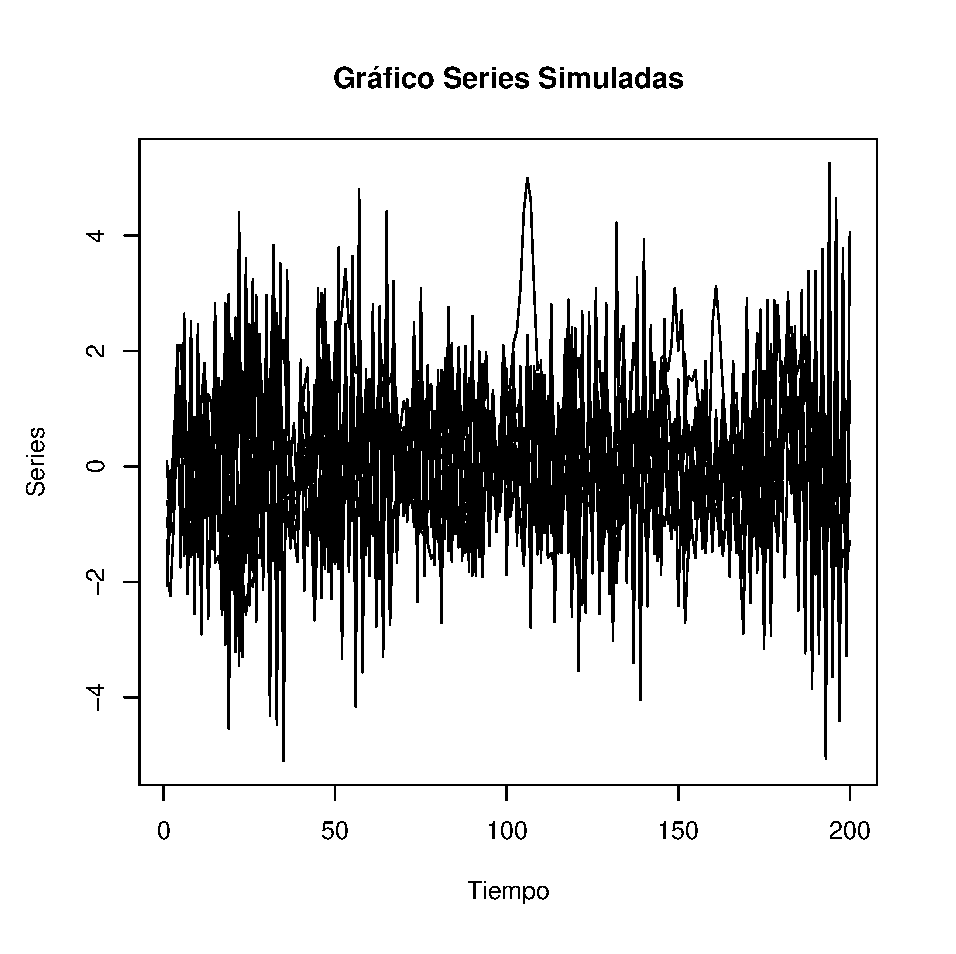
\includegraphics[height=4cm, width=6cm]{s_simu.eps}}
\caption{Series simuladas}
\label{caja}
\end{figure}

En este gr\'afico se puede observar un conjunto de series estacionarias.\\

\begin{figure}[!htp]
\centering
\fbox{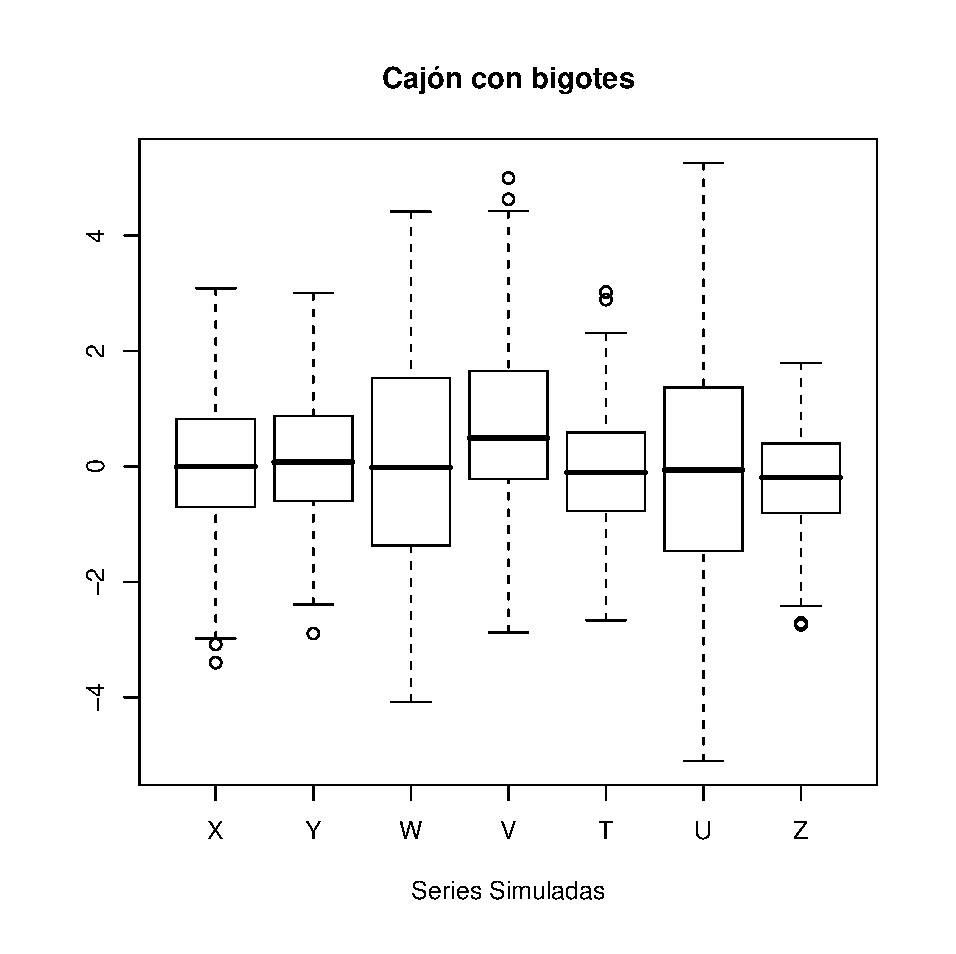
\includegraphics[height=4cm, width=6cm]{cajon_simu.eps}}
\caption{Series simuladas}
\label{caja}
\end{figure}

\newpage
Adem\'as, si aplicamos el algoritmo de clasificaci\'on con las distancias convencionales, se pueden obtener los siguientes resultados.

\begin{figure}[!htp]
\centering
\fbox{ 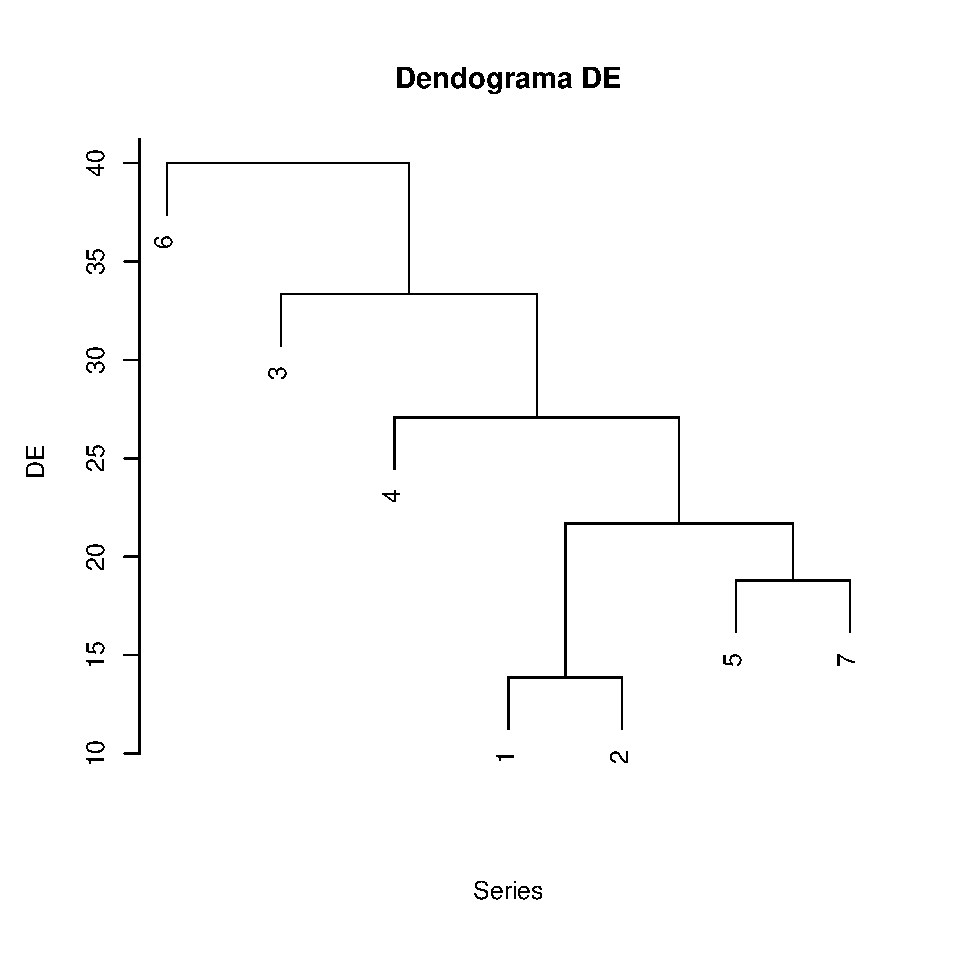
\includegraphics[height=4cm, width=4cm]{de.eps}
       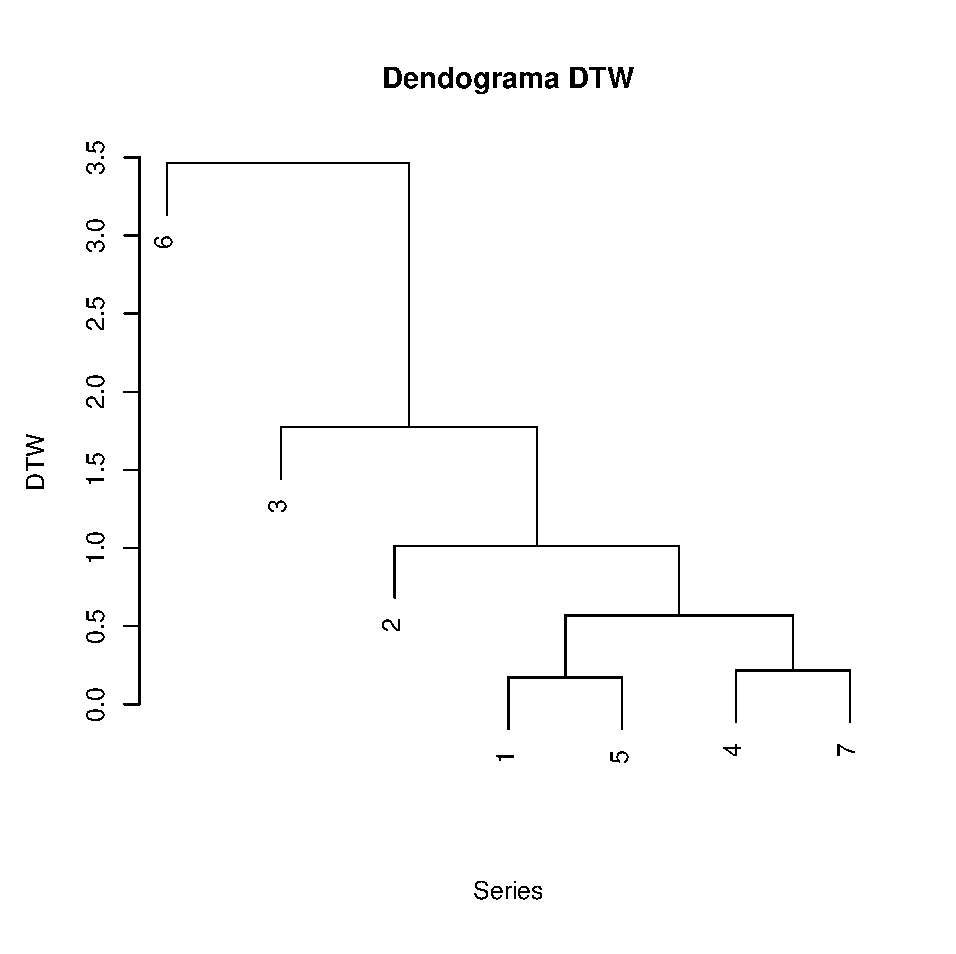
\includegraphics[height=4cm, width=4cm]{dtw.eps}
       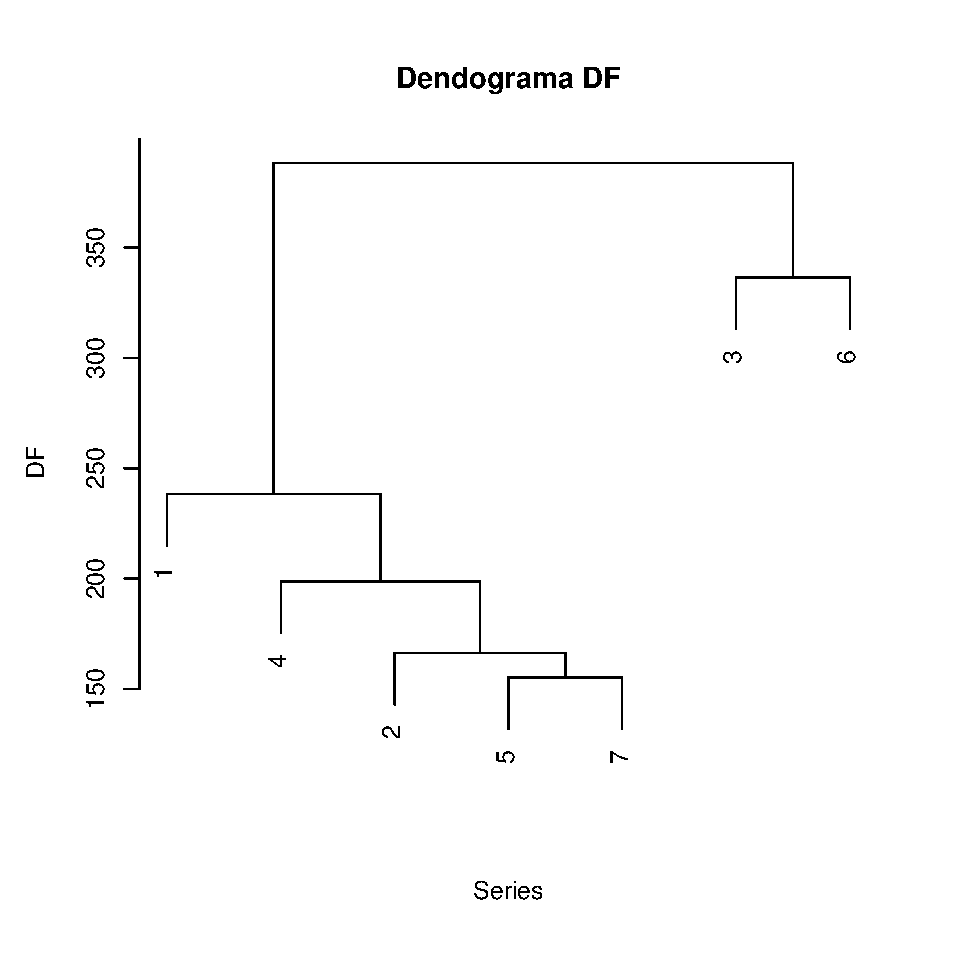
\includegraphics[height=4cm, width=4cm]{df.eps}}
\caption{Dendogramas.}
\label{caja}
\end{figure}

En base a la informaci\'on de las distancias convencionales y con el algoritmo de clasificaci\'on utilizando el m\'etodo jer\'arquico, del vecino m\'as cercano, se puede decir que la distancia euclidiana agrupa 2 de las 3 series correlacionadas, en cambio las distancias de Frech\'et y DTW no agrupan ninguna de las series con errores correlacionados.

\subsection{Gr\'aficos Camino Distorsionado}

Una caracter\'istica que tiene la distancia DTW, es gr\'aficar la opci\'on de camino distorsionado entre las series, a continuaci\'on se presentar\'an algunos gr\'aficos con distintas combinaciones entre las distintas series y analizar la similitud entre las series.

\begin{figure}[!htp]
       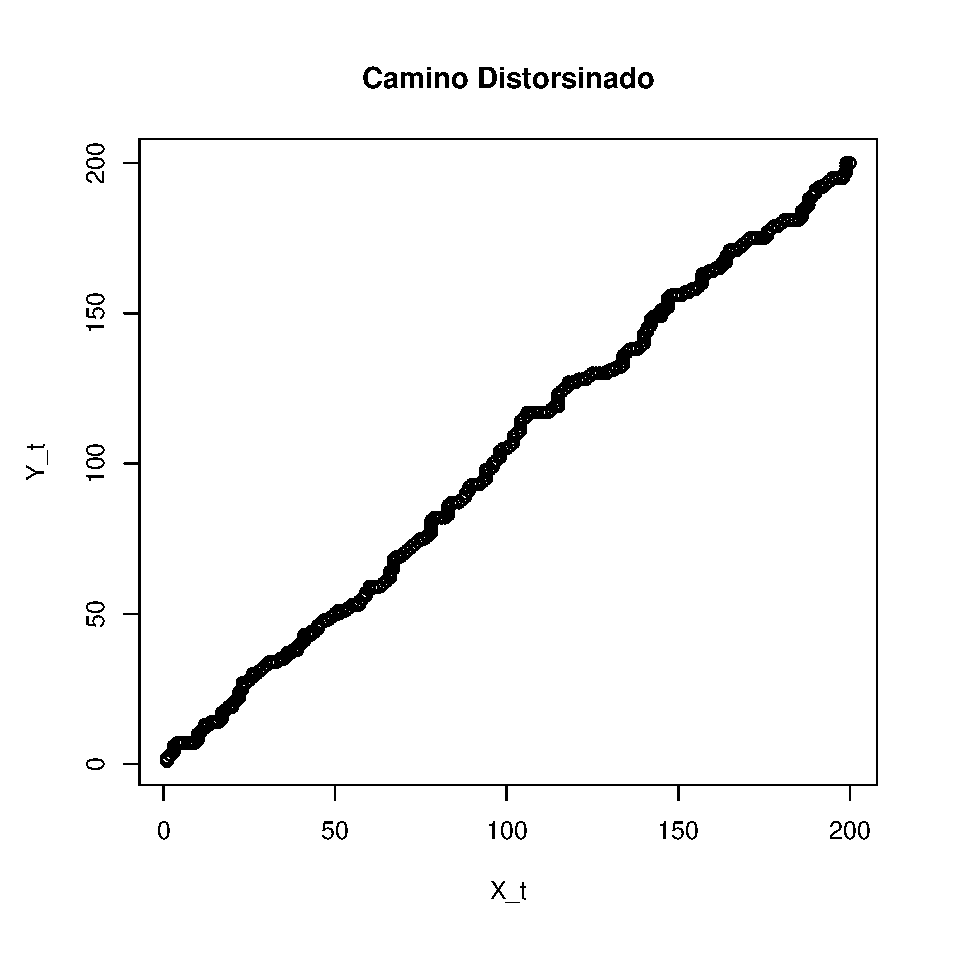
\includegraphics[height=4cm, width=4cm]{cam_dist_xy.eps}
       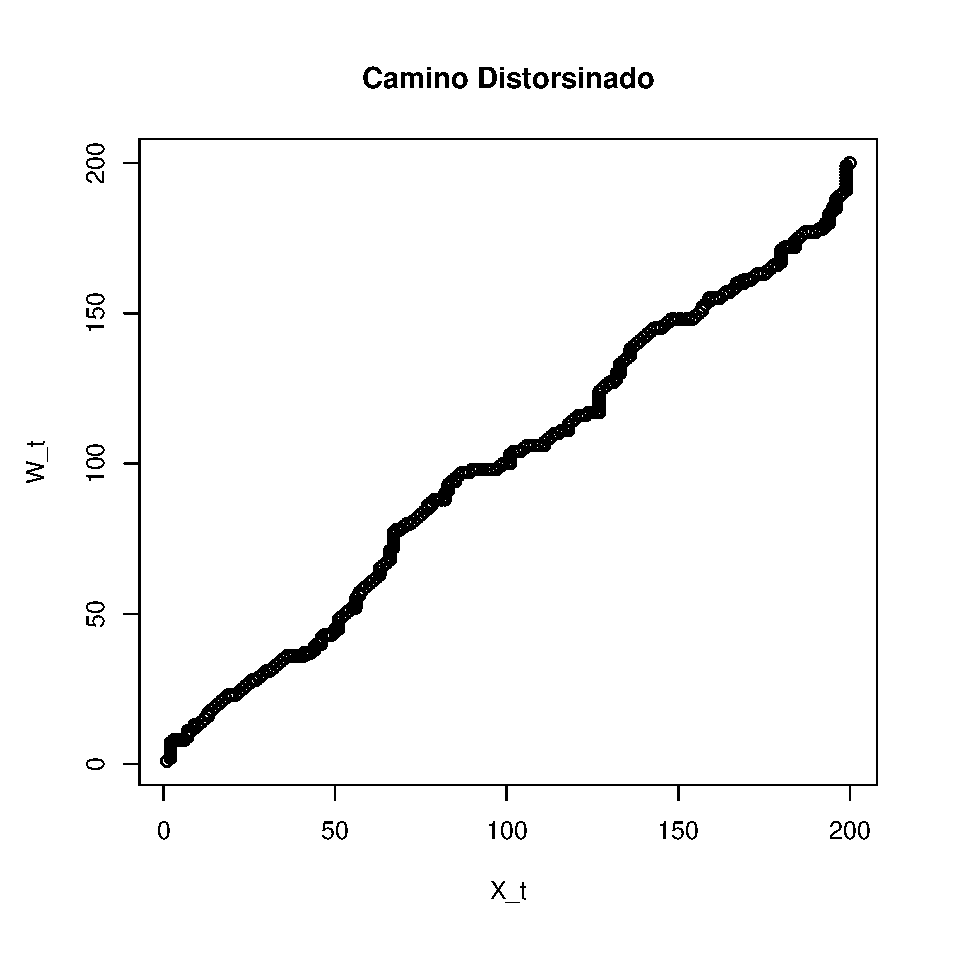
\includegraphics[height=4cm, width=4cm]{cam_dist_xw.eps}
       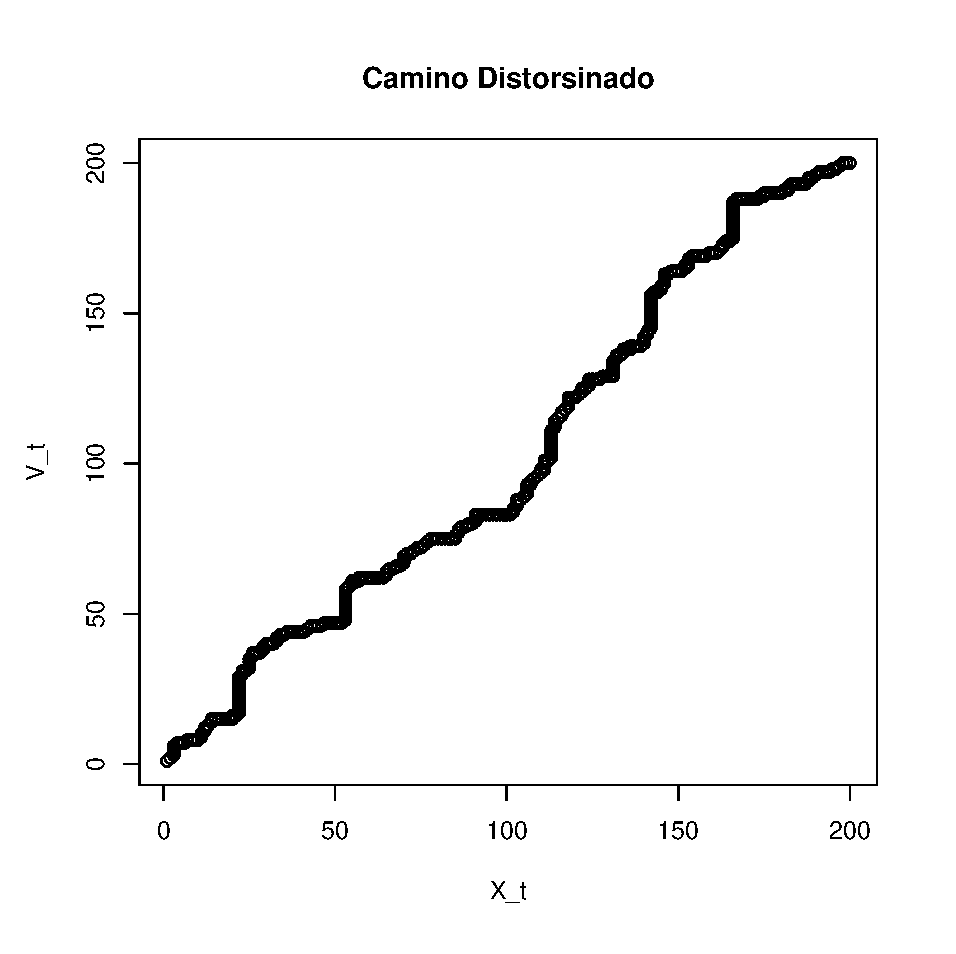
\includegraphics[height=4cm, width=4cm]{cam_dist_xv.eps}
       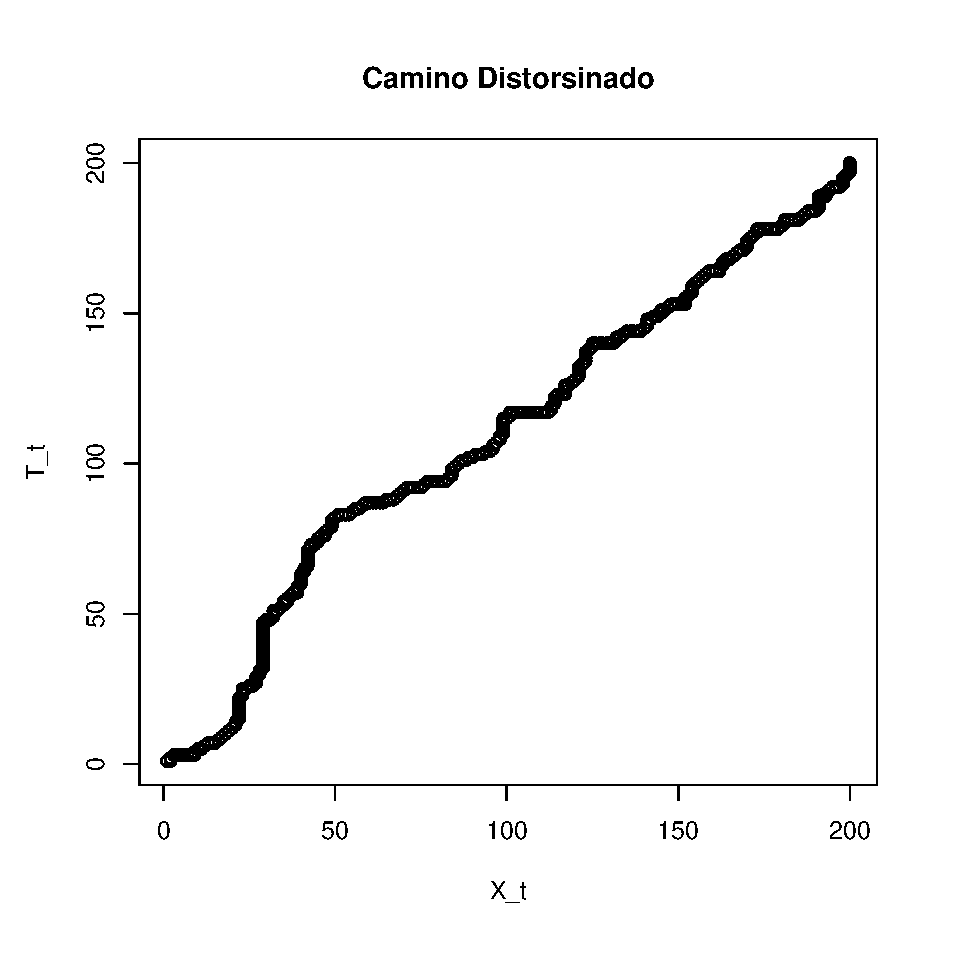
\includegraphics[height=4cm, width=4cm]{cam_dist_xt.eps}
       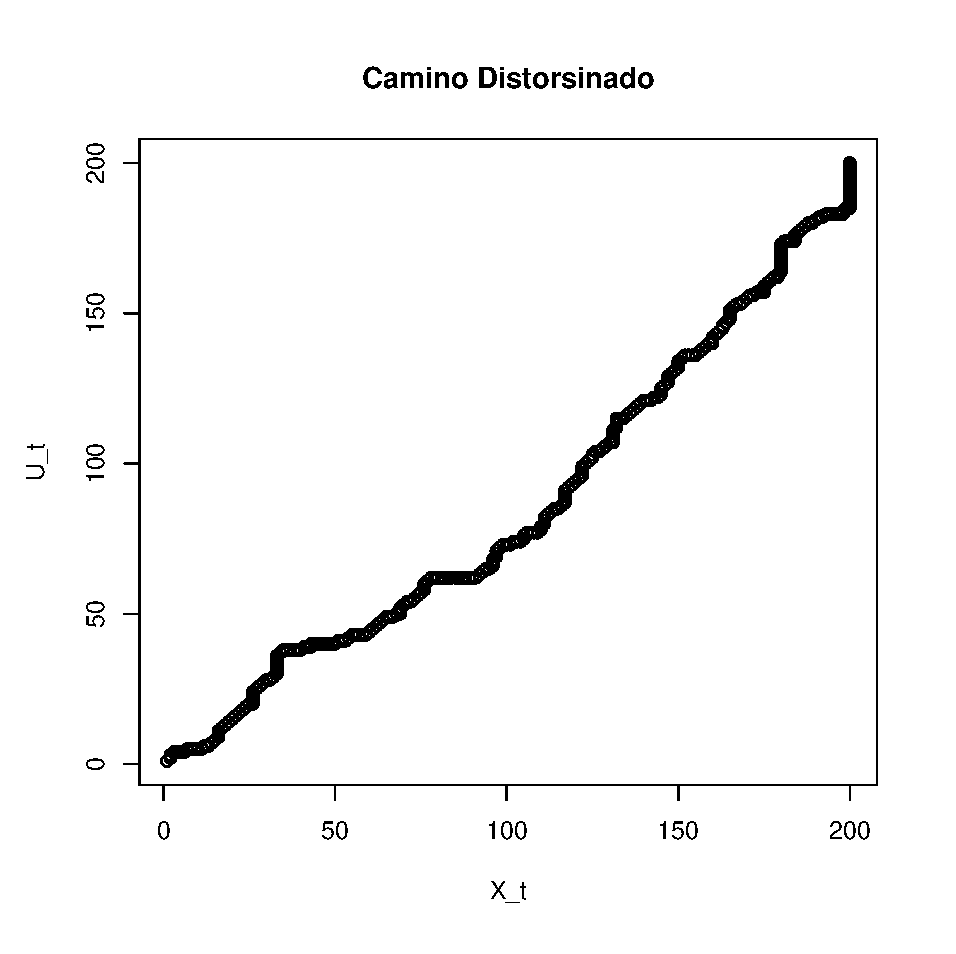
\includegraphics[height=4cm, width=4cm]{cam_dist_xu.eps}
       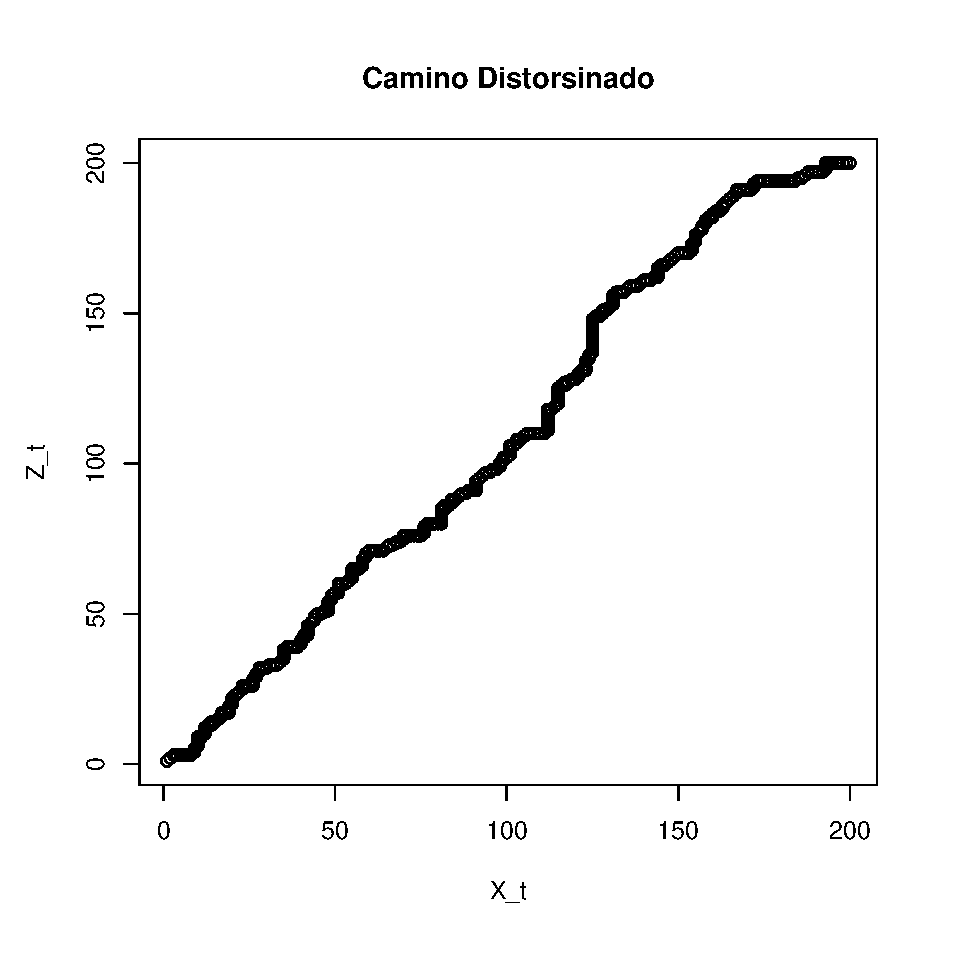
\includegraphics[height=4cm, width=4cm]{cam_dist_xz.eps}
\caption{Camino Distorsionado.}
\label{caja}
\end{figure}

Estos gr\'aficos nos dan una idea de como interactuan las series, se puede apreciar un grado de similitud entre las series, ya que, los puntos del camino distorsionado presentan una recta.\\

Por otra parte, si se aplica el algoritmo de clasificaci\'on con el \'Indice de Disimilaridad Adaptativo con $h=1,2,3$ y $k=1,2,3,4$ se puede observar los siguientes resultados.

\subsection{\'Indice de Disimilaridad Adaptativo con Distancia Euclidiana}

En base a la simulaci\'on y el c\'alculo de las matrices de distancia con esta nueva medida de clasificaci\'on se puede apreciar los siguientes resultados.

El \'Indice con $h=1$ agrupa las series $X_t$, $Y_t$ y $W_t$, como era de esperar, agrupa primero $X_t$ con $Y_t$, ya que sus errores tienen un grado m\'as alto de correlaci\'on, luego incorpora la series $W_t$. A continuaci\'on se presenta el algoritmo de clasificaci\'on para series temporales con $h=2,3$. Se puede observar que para $h=2$, el \'Indice de Disimilaridad mantiene los grupos, que est\'an correlacionados. Con $h=3$, el \'Indice de Disimilaridad mantiene los grupos establecidos.

\begin{figure}[!htp]
       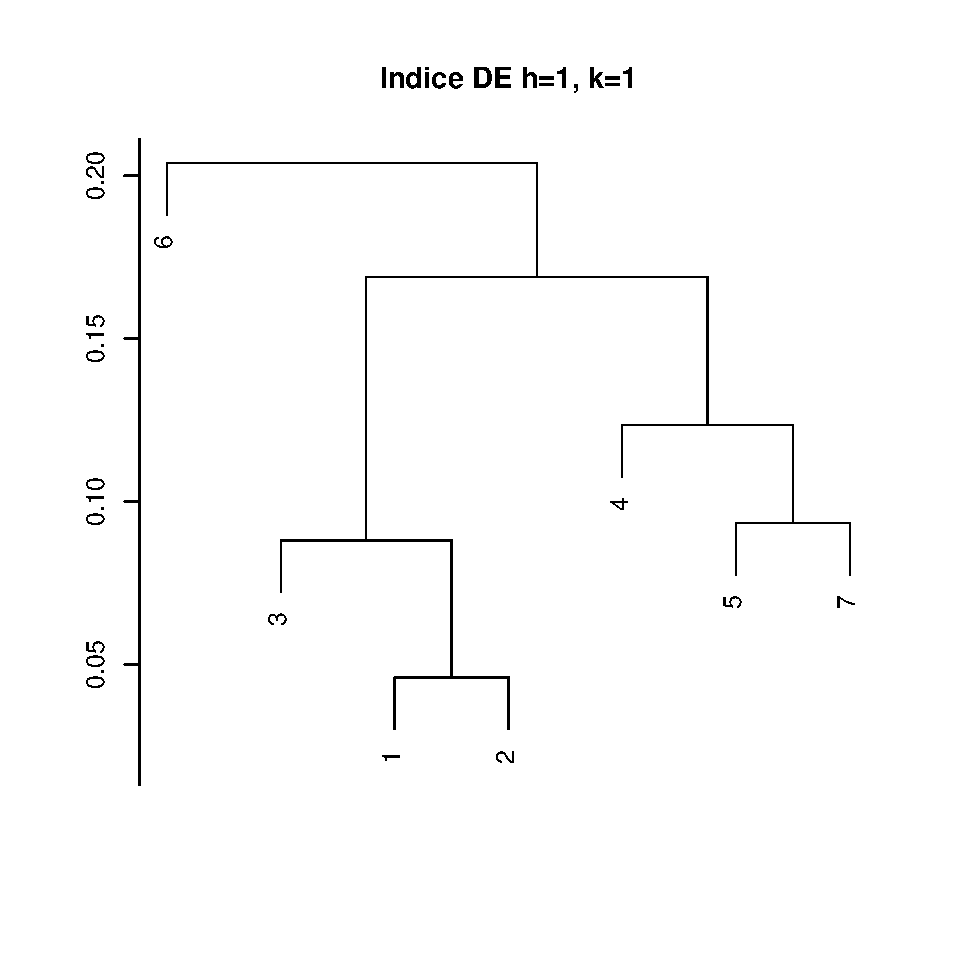
\includegraphics[height=4cm, width=4cm]{d111.eps}
       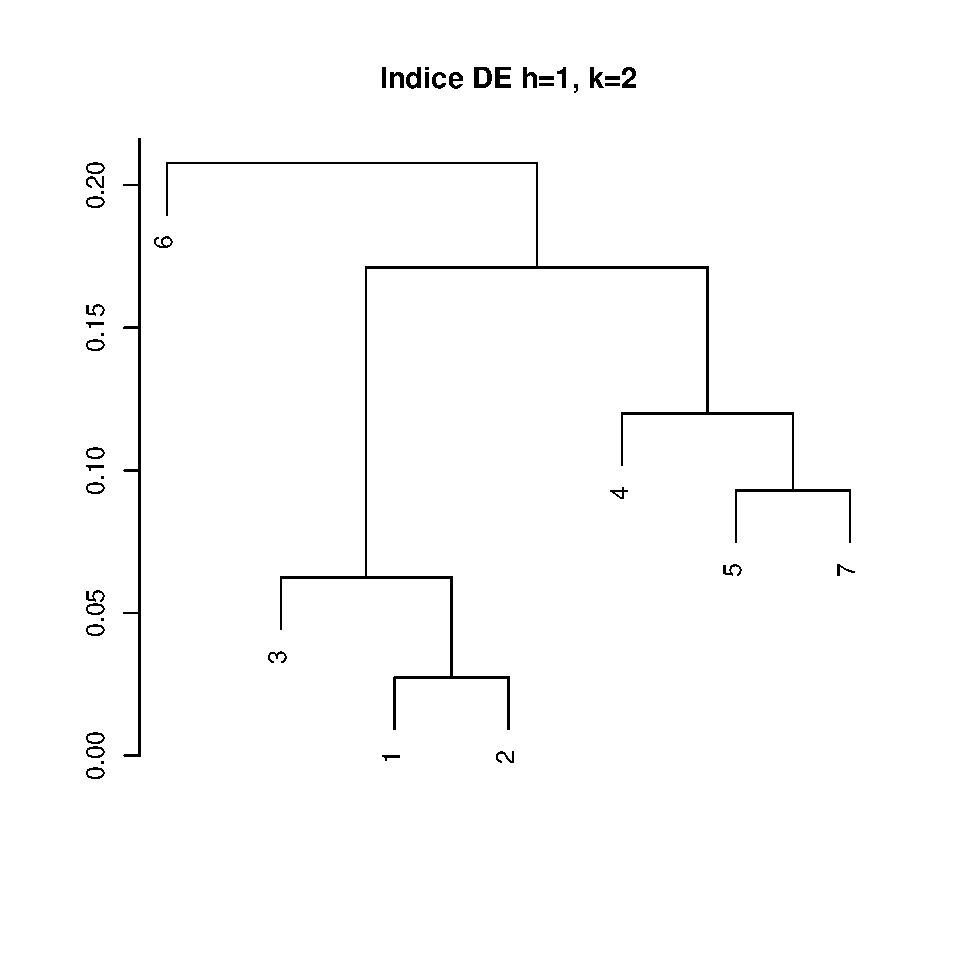
\includegraphics[height=4cm, width=4cm]{d112.eps}
       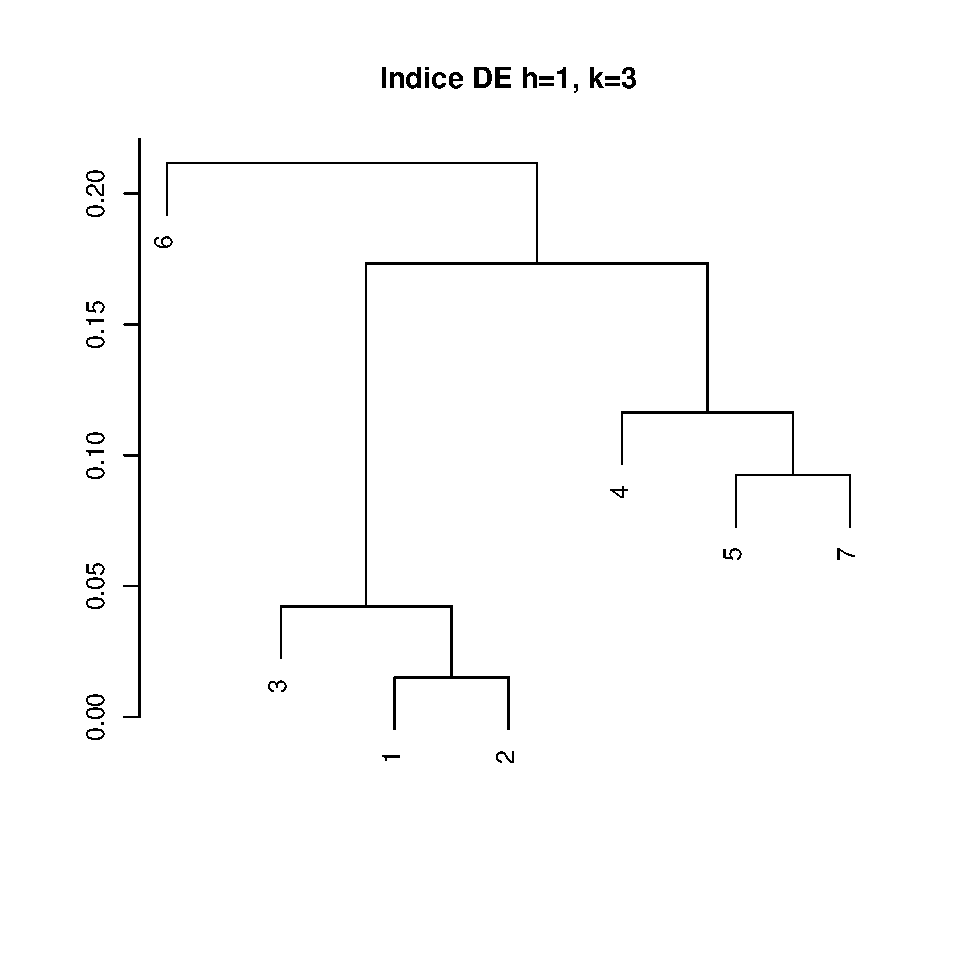
\includegraphics[height=4cm, width=4cm]{d113.eps}
       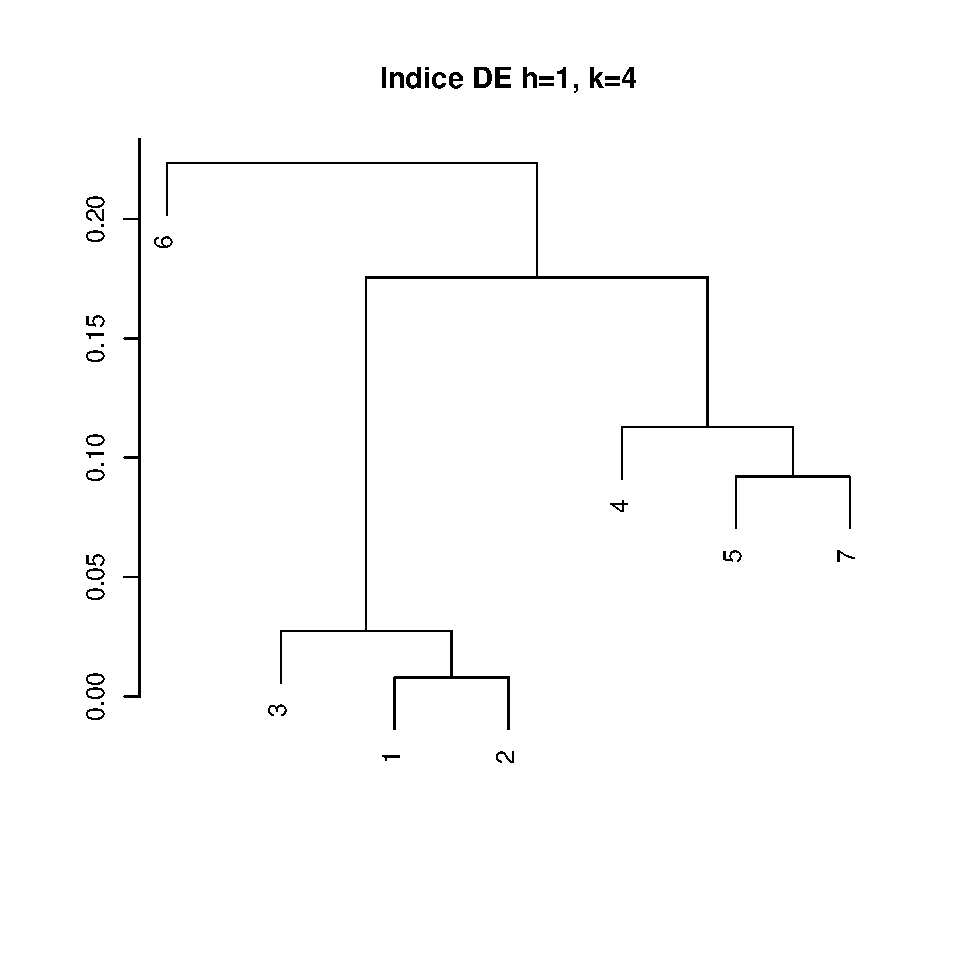
\includegraphics[height=4cm, width=4cm]{d114.eps}
\caption{Dendogramas \'Indice con $\delta_{E}$ con $h=1$, $k=1,2,3,4.$}
\label{caja}
\end{figure}


\begin{figure}[!htp]
       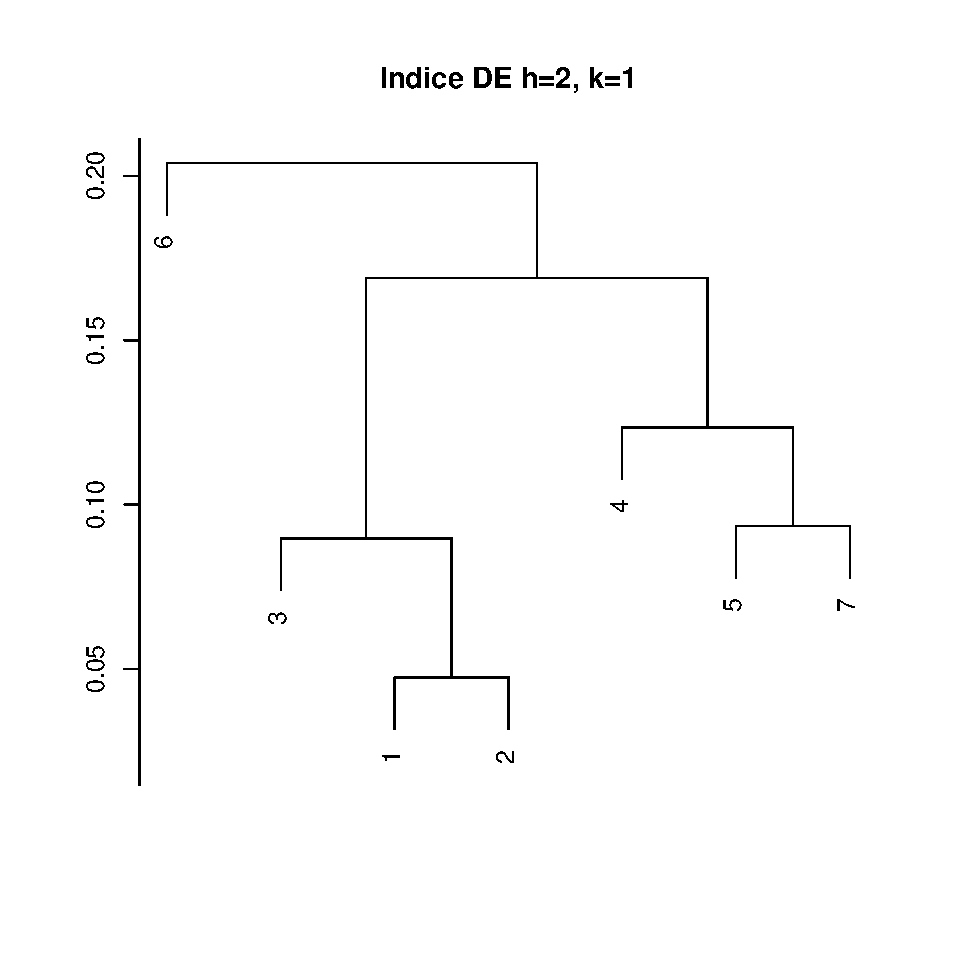
\includegraphics[height=4cm, width=4cm]{d121.eps}
       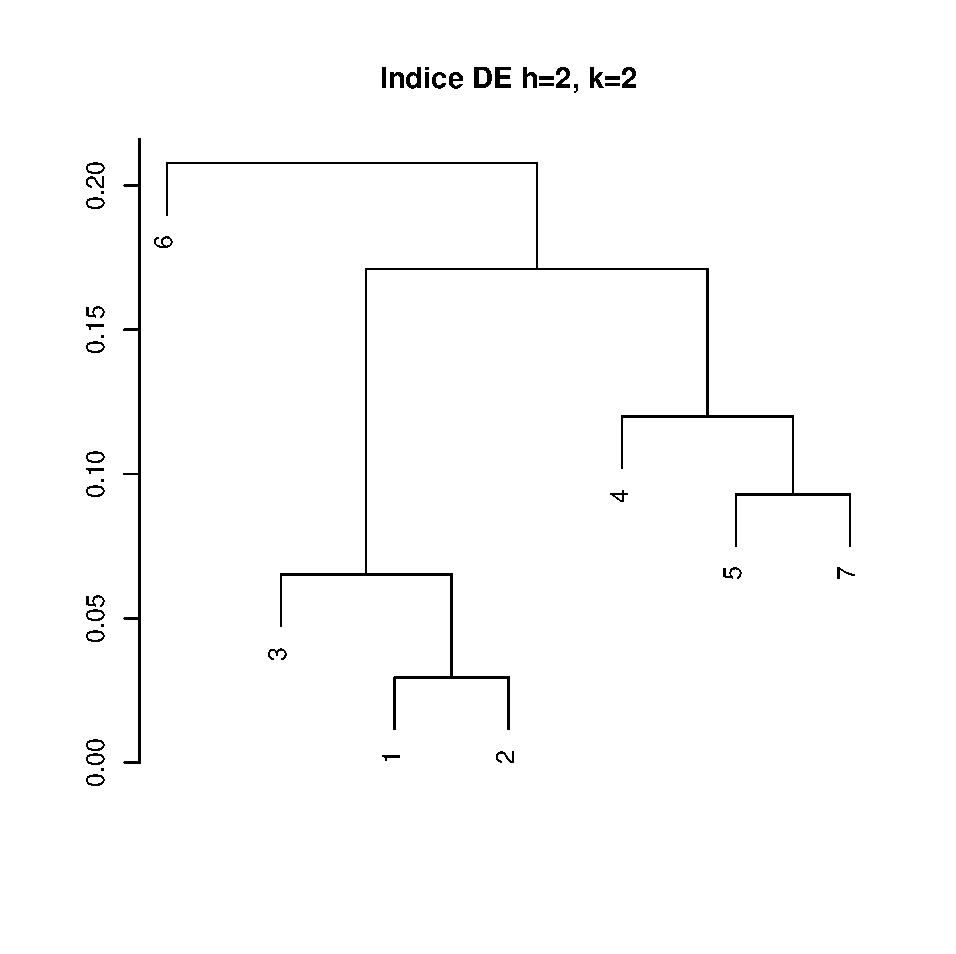
\includegraphics[height=4cm, width=4cm]{d122.eps}
       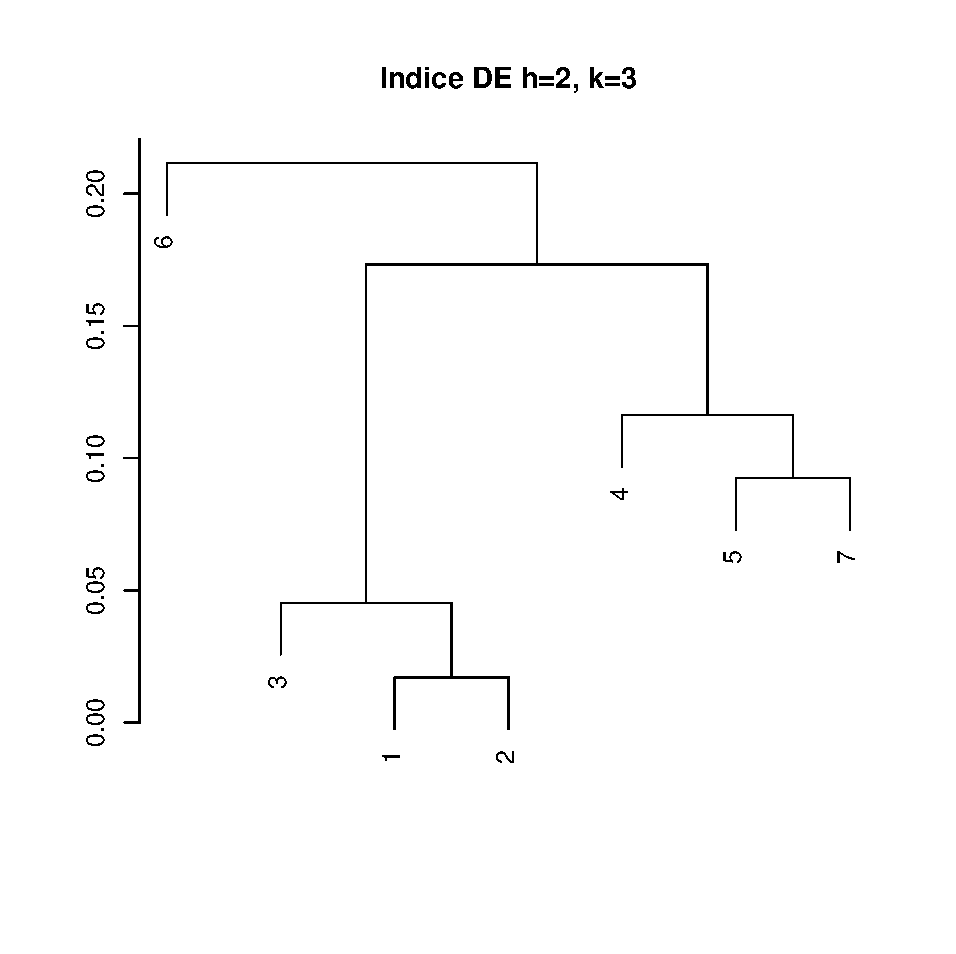
\includegraphics[height=4cm, width=4cm]{d123.eps}
       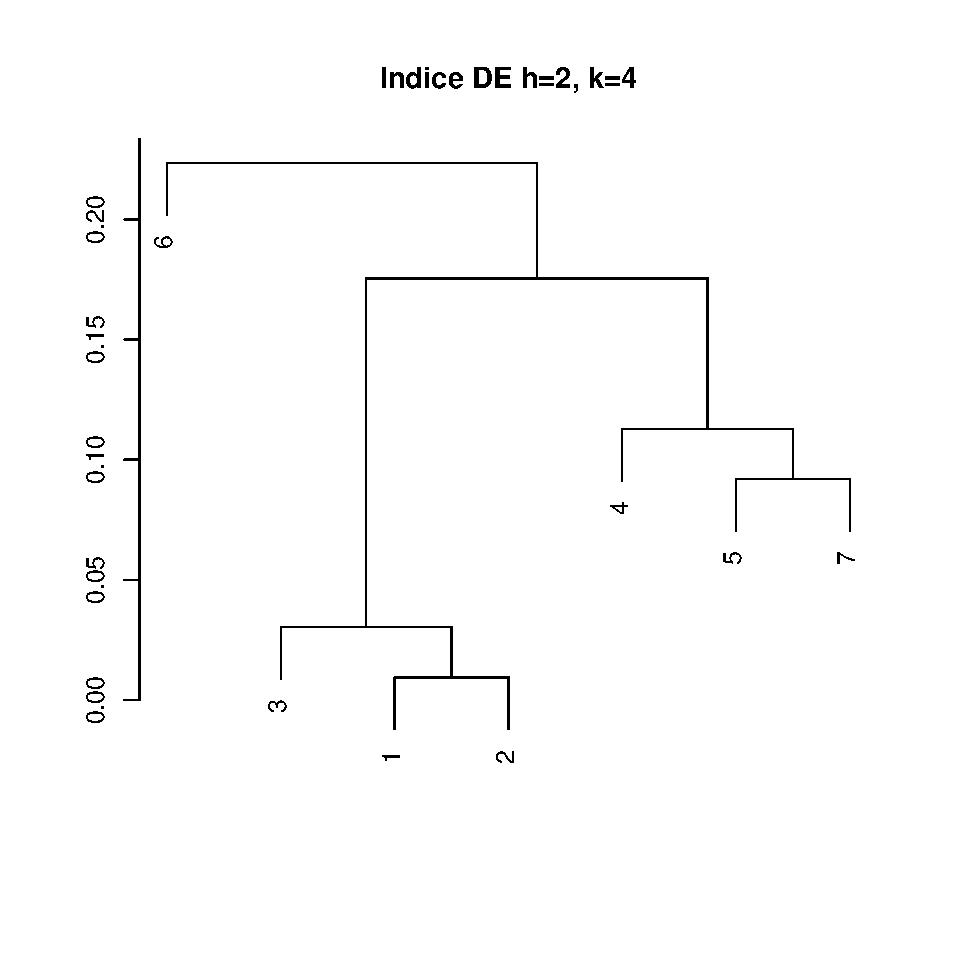
\includegraphics[height=4cm, width=4cm]{d124.eps}
\caption{Dendogramas \'Indice con $\delta_{E}$ con $h=2$, $k=1,2,3,4.$}
\label{caja}
\end{figure}


\begin{figure}[!htp]
       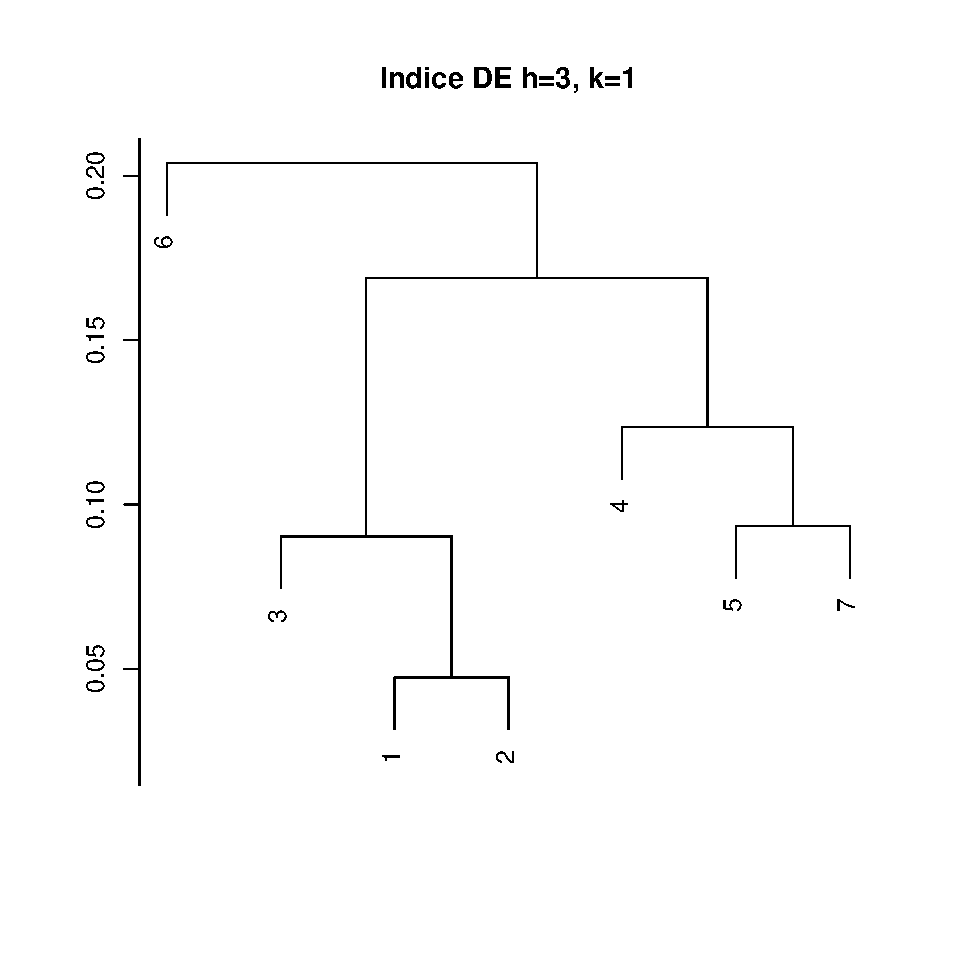
\includegraphics[height=4cm, width=4cm]{d131.eps}
       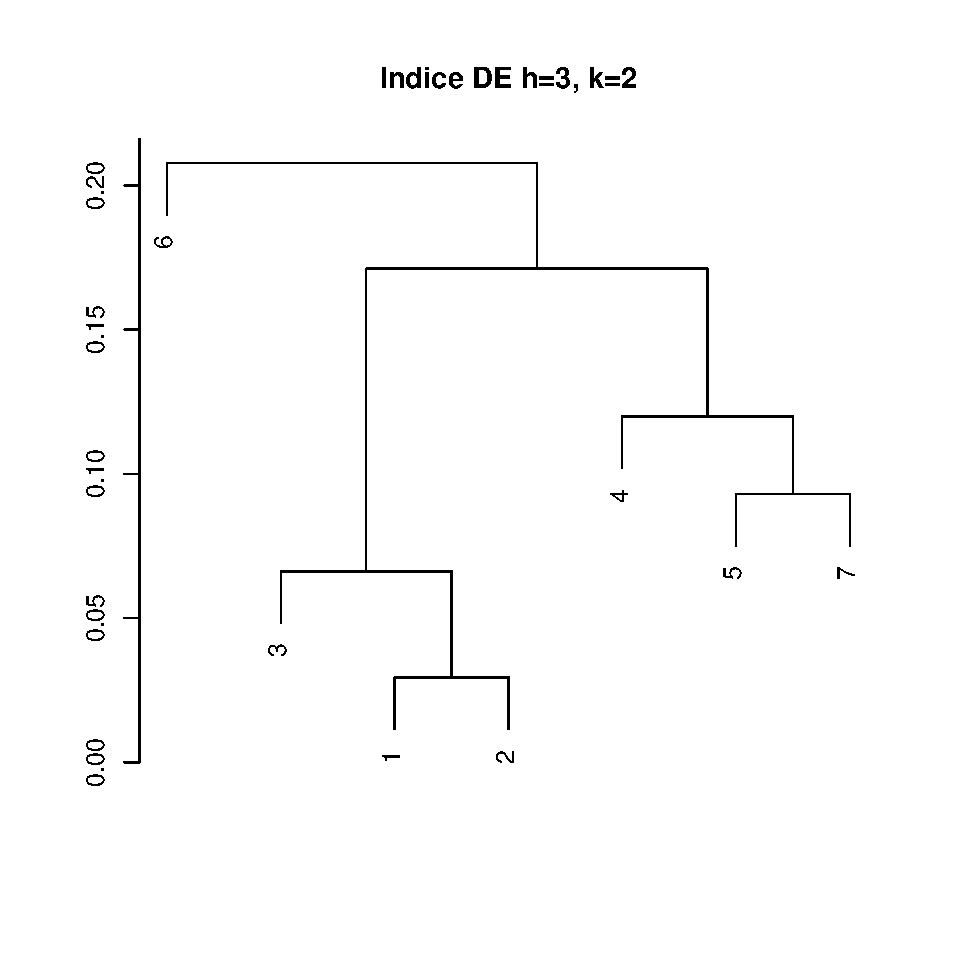
\includegraphics[height=4cm, width=4cm]{d132.eps}
       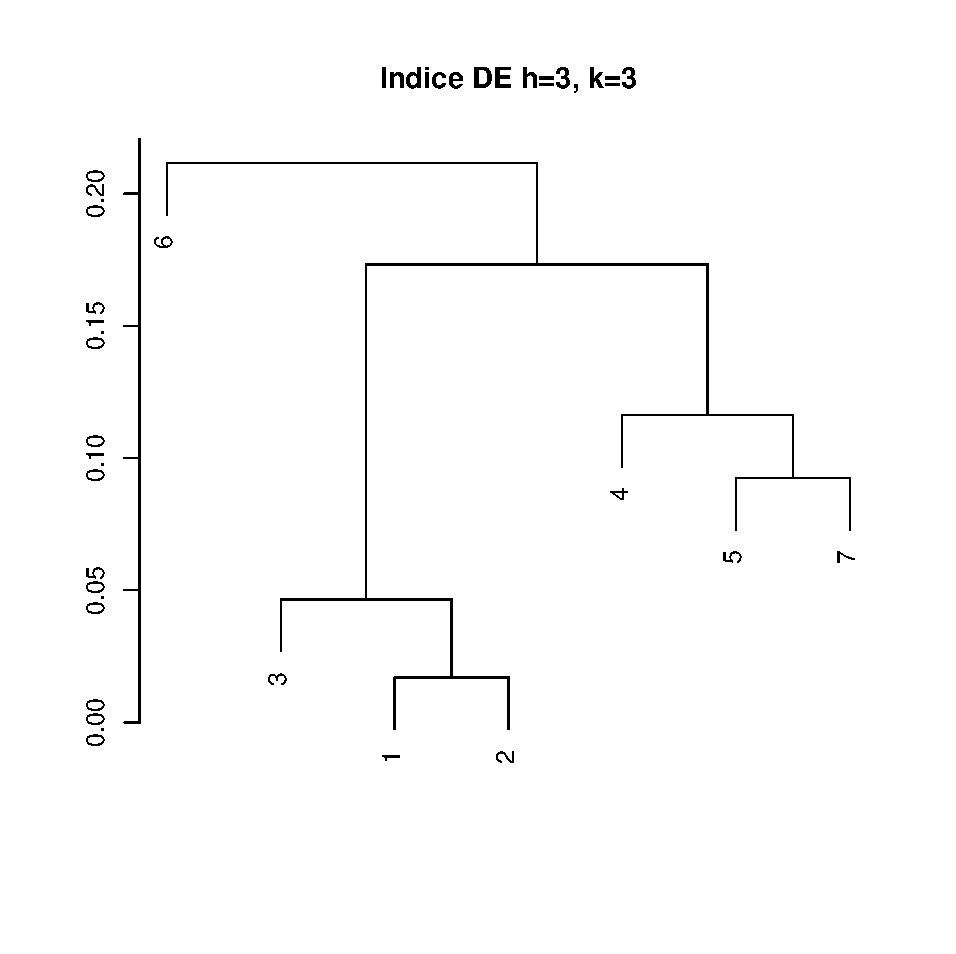
\includegraphics[height=4cm, width=4cm]{d133.eps}
       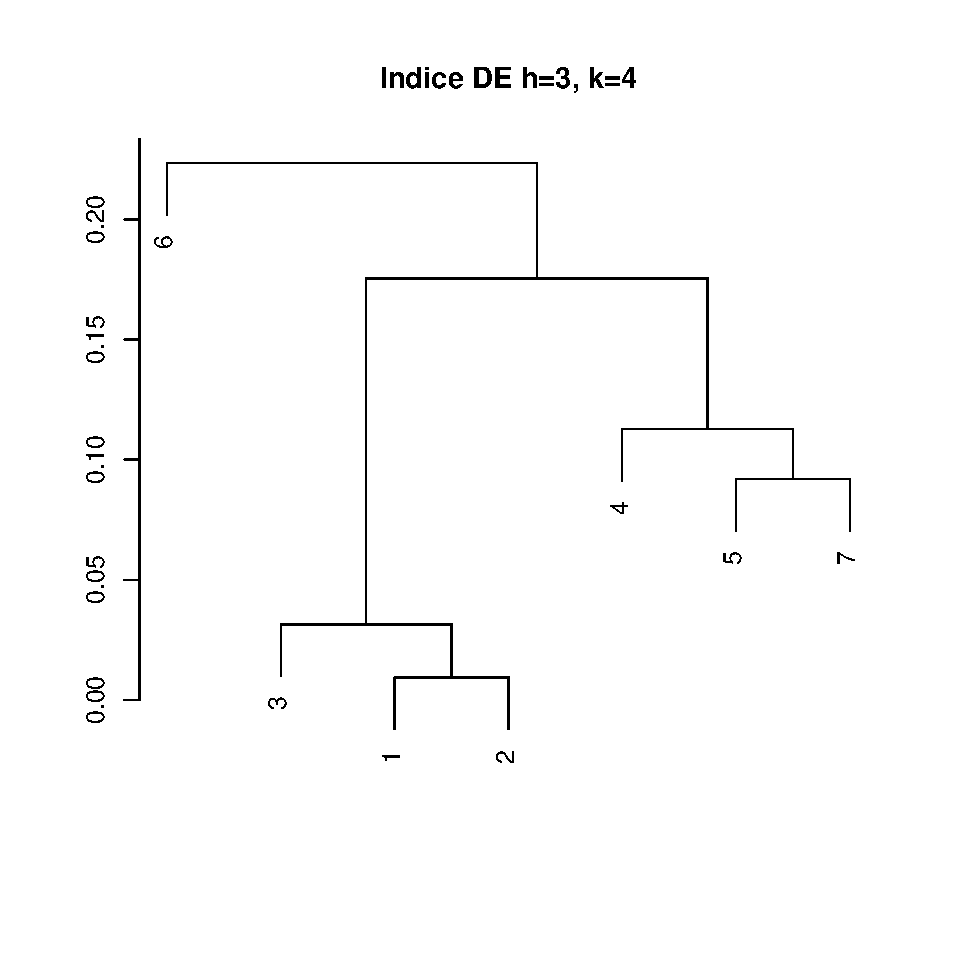
\includegraphics[height=4cm, width=4cm]{d134.eps}
\caption{Dendogramas \'Indice con $\delta_{E}$ con $h=3$, $k=1,2,3,4.$}
\label{caja}
\end{figure}


\subsection{\'Indice de Disimilaridad Adaptativo con Distancia DTW}
De igual forma que anteriormente calculamos el \'Indice de Disimilaridad Adaptativo con la Distancia  DTW con $h=1,2,3$ y $k=1,2,3,4$, se observan los siguientes resultados.

\begin{figure}[!htp]
       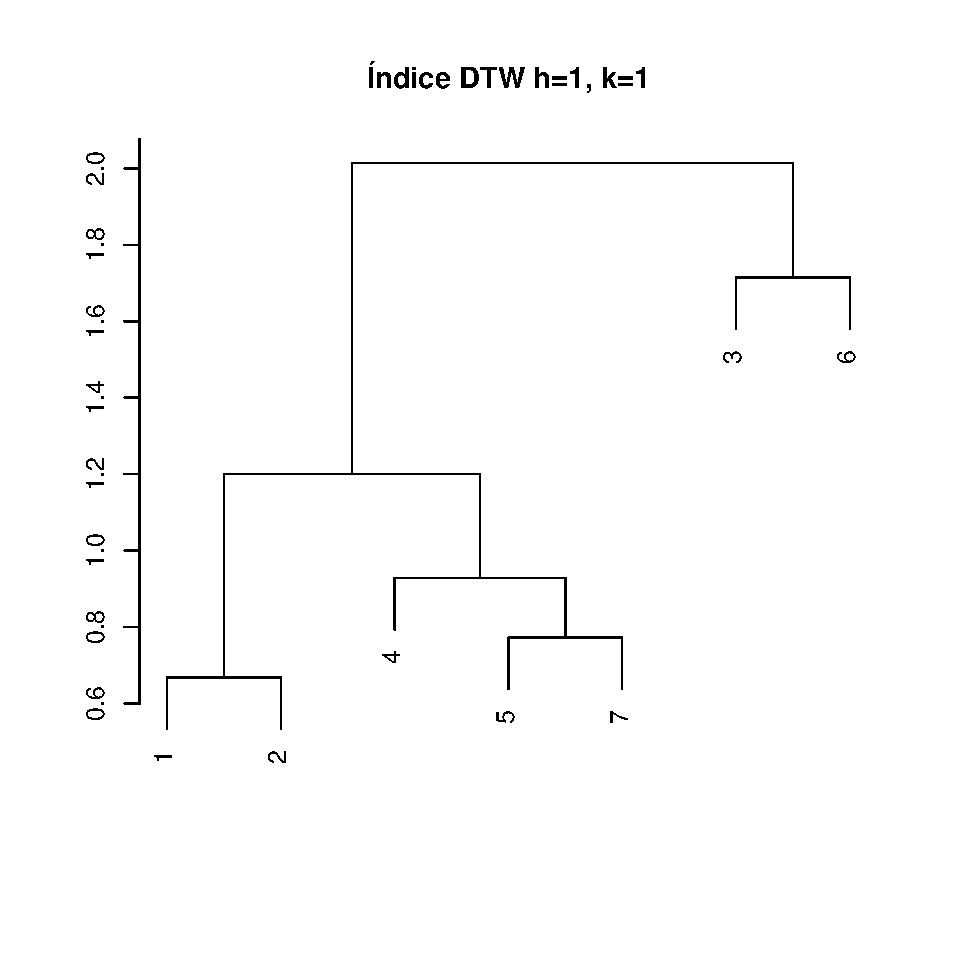
\includegraphics[height=4cm, width=4cm]{d211.eps}
       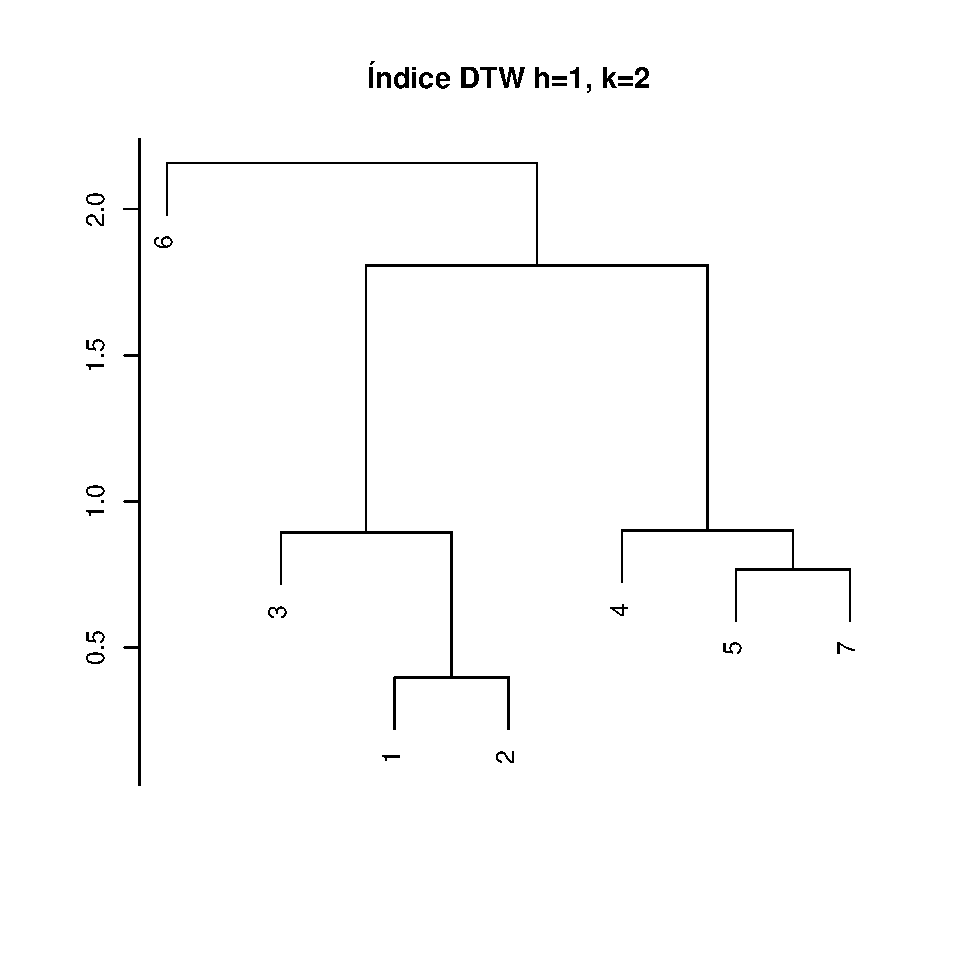
\includegraphics[height=4cm, width=4cm]{d212.eps}
       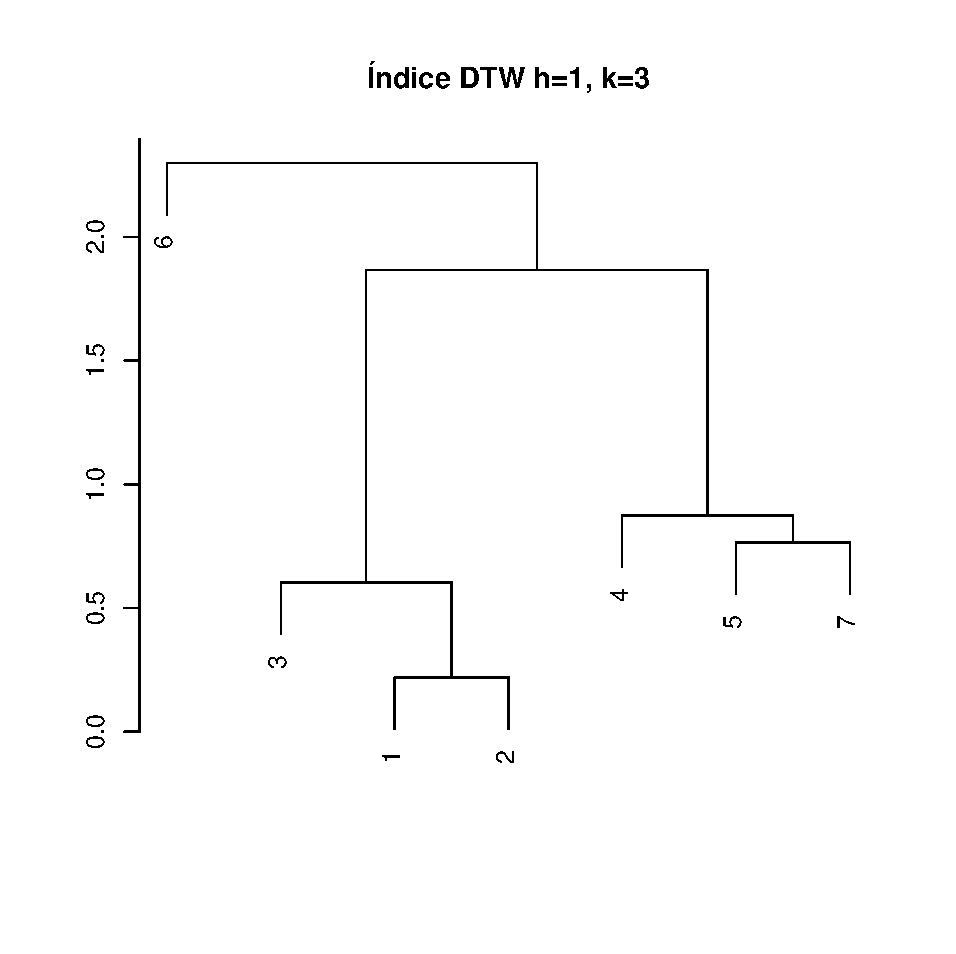
\includegraphics[height=4cm, width=4cm]{d213.eps}
       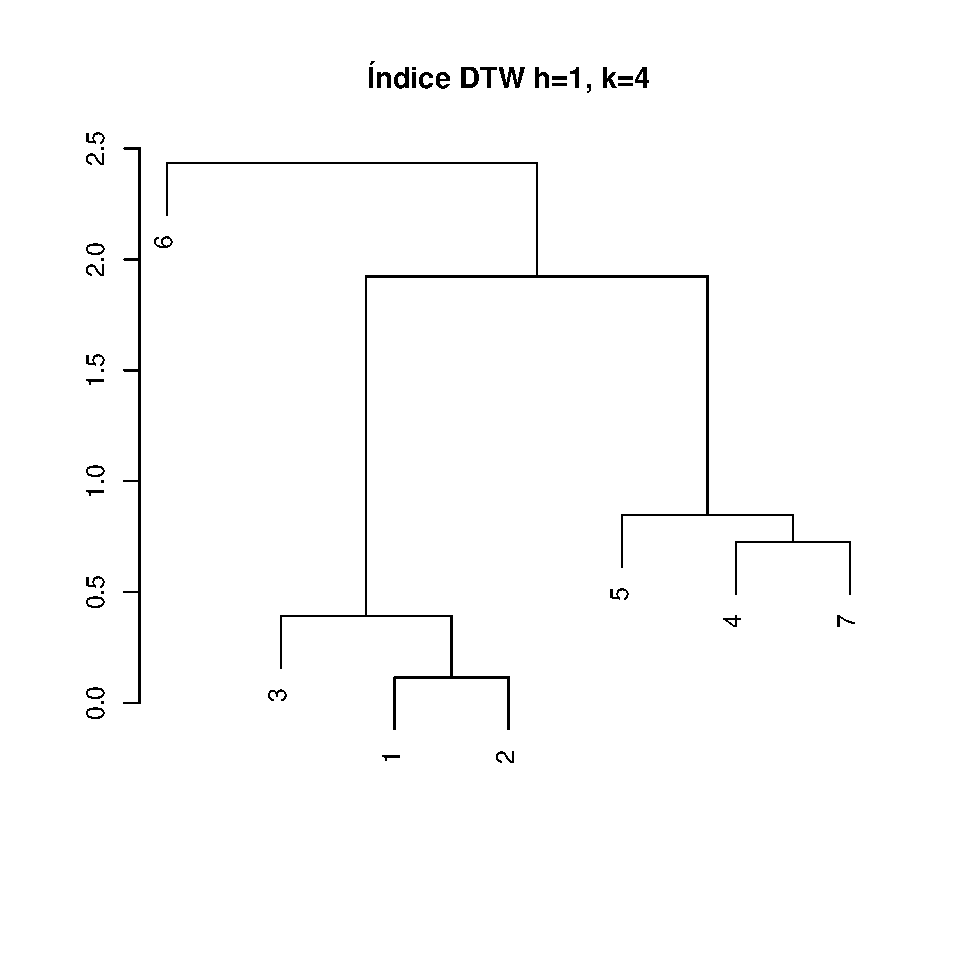
\includegraphics[height=4cm, width=4cm]{d214.eps}
\caption{Dendogramas \'Indice con $\delta_{DTW}$ con $h=1$, $k=1,2,3,4.$}
\label{caja}
\end{figure}

En el este caso con $h=1$ y $k=1$, el \'Indice no agrup\'o las series esperadas. No obstante, con $k=2,3$, el \'Indice agrupa las series esperadas.

\begin{figure}[!htp]
       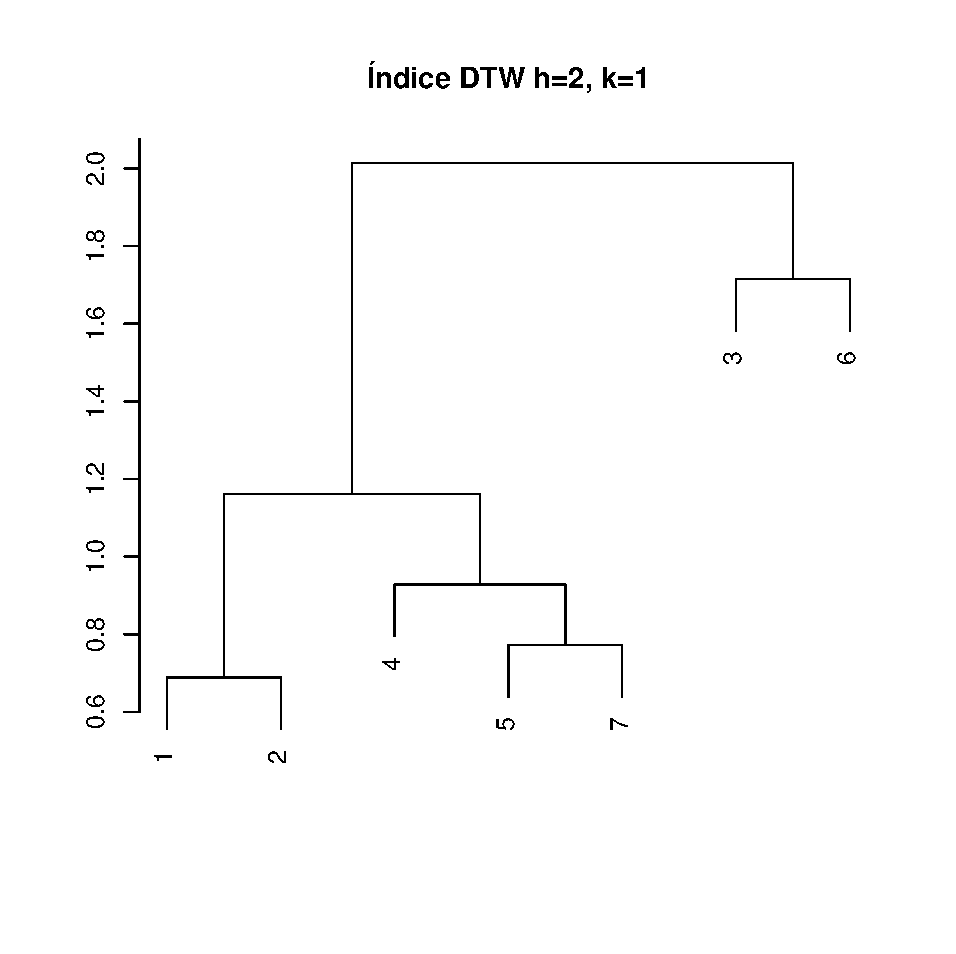
\includegraphics[height=4cm, width=4cm]{d221.eps}
       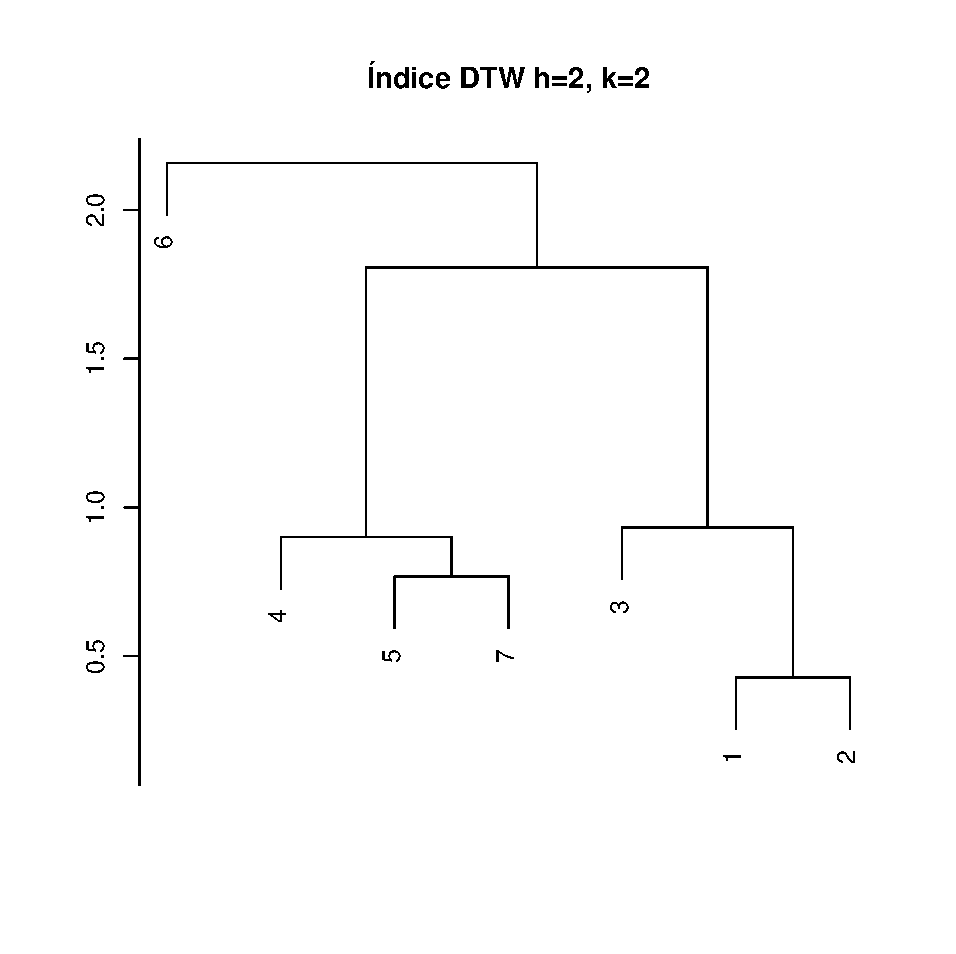
\includegraphics[height=4cm, width=4cm]{d222.eps}
       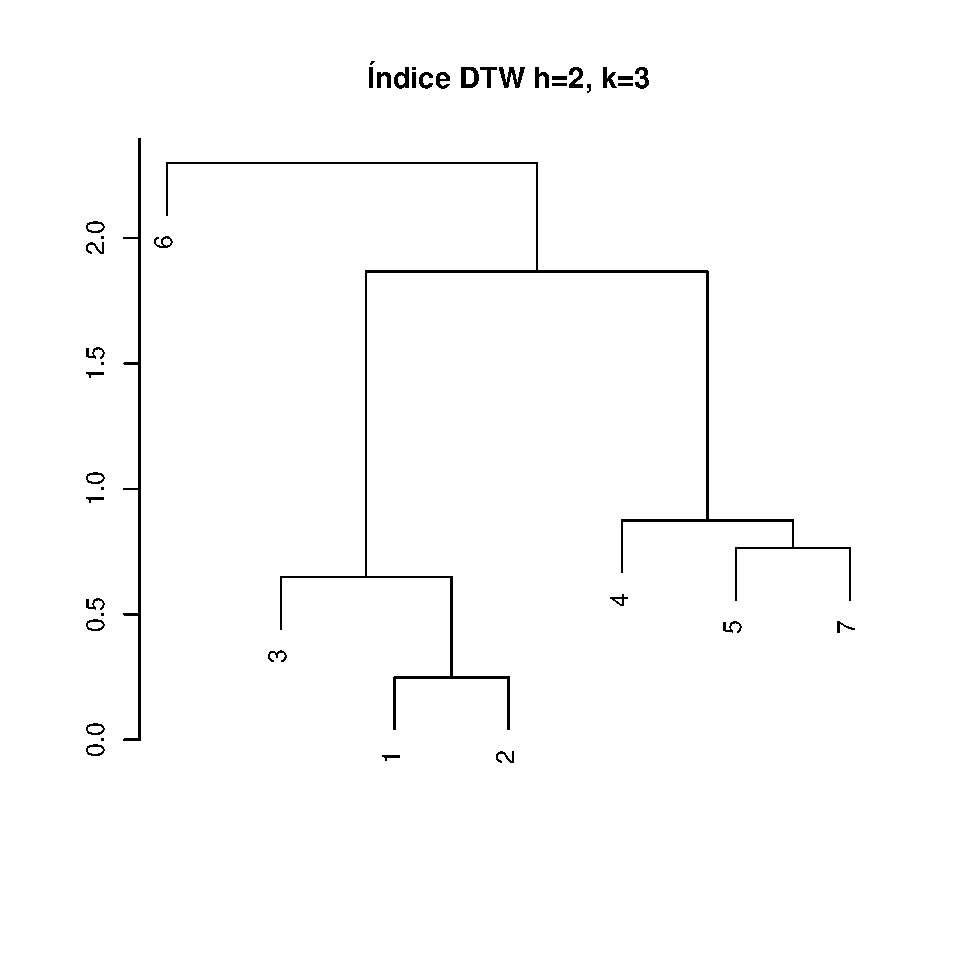
\includegraphics[height=4cm, width=4cm]{d223.eps}
       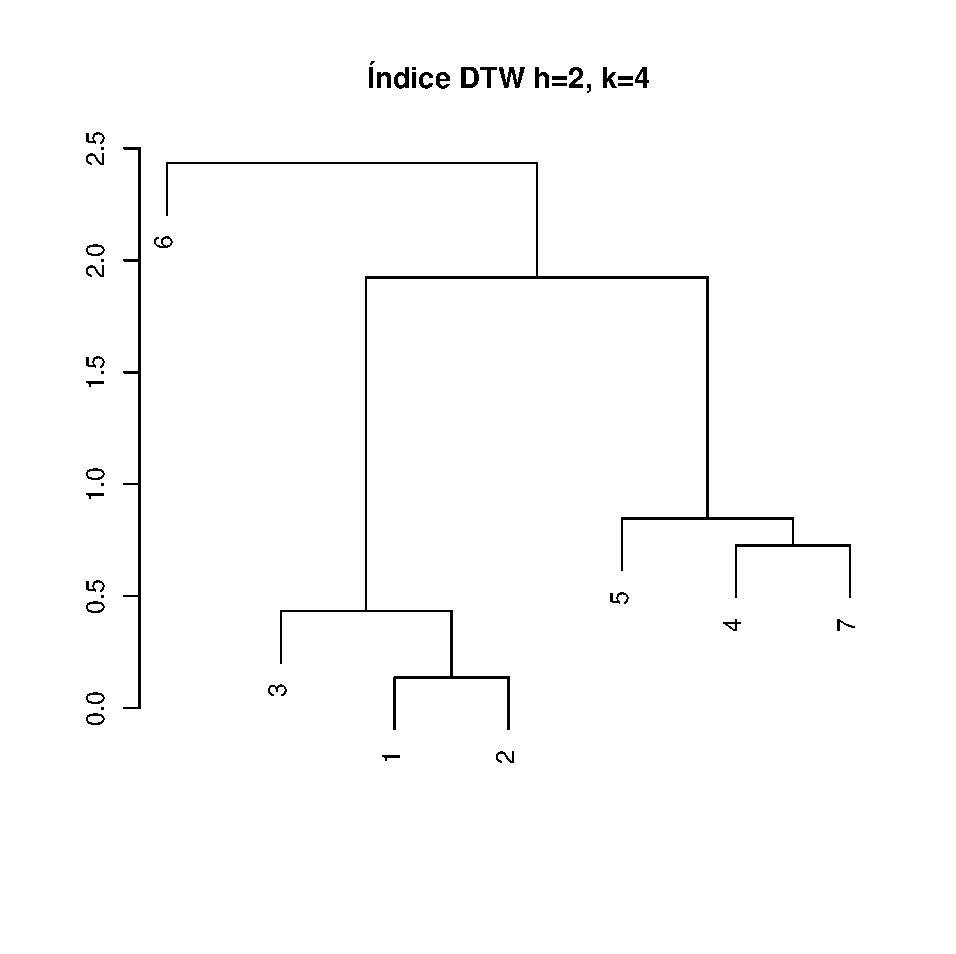
\includegraphics[height=4cm, width=4cm]{d224.eps}
\caption{Dendogramas \'Indice con $\delta_{DTW}$ con $h=2$, $k=1,2,3,4.$}
\label{caja}
\end{figure}

\begin{figure}[!htp]
       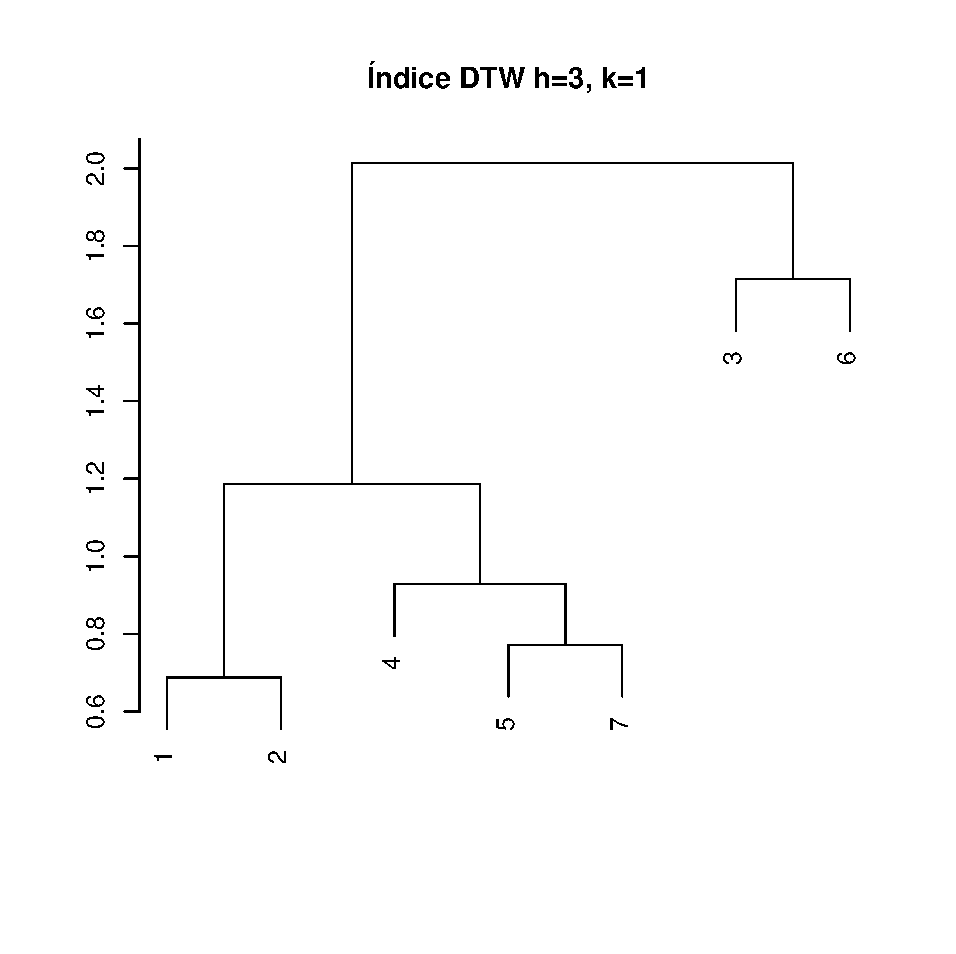
\includegraphics[height=4cm, width=4cm]{d231.eps}
       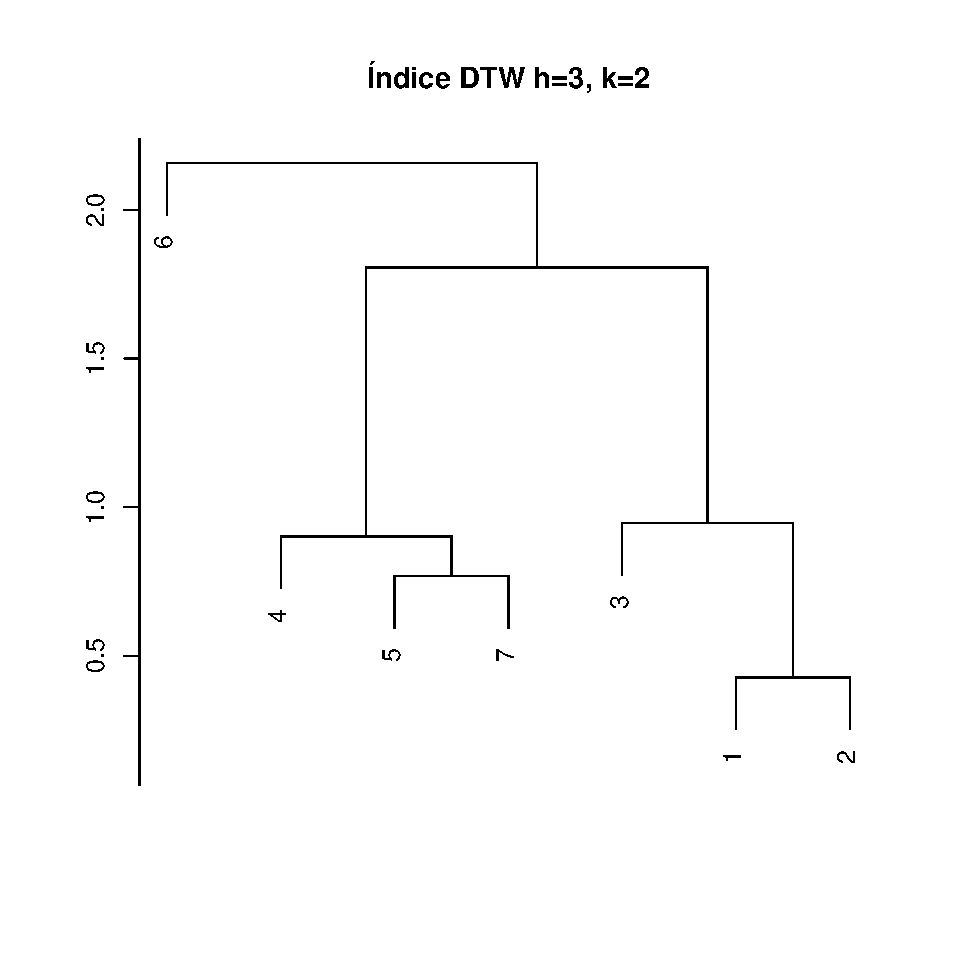
\includegraphics[height=4cm, width=4cm]{d232.eps}
       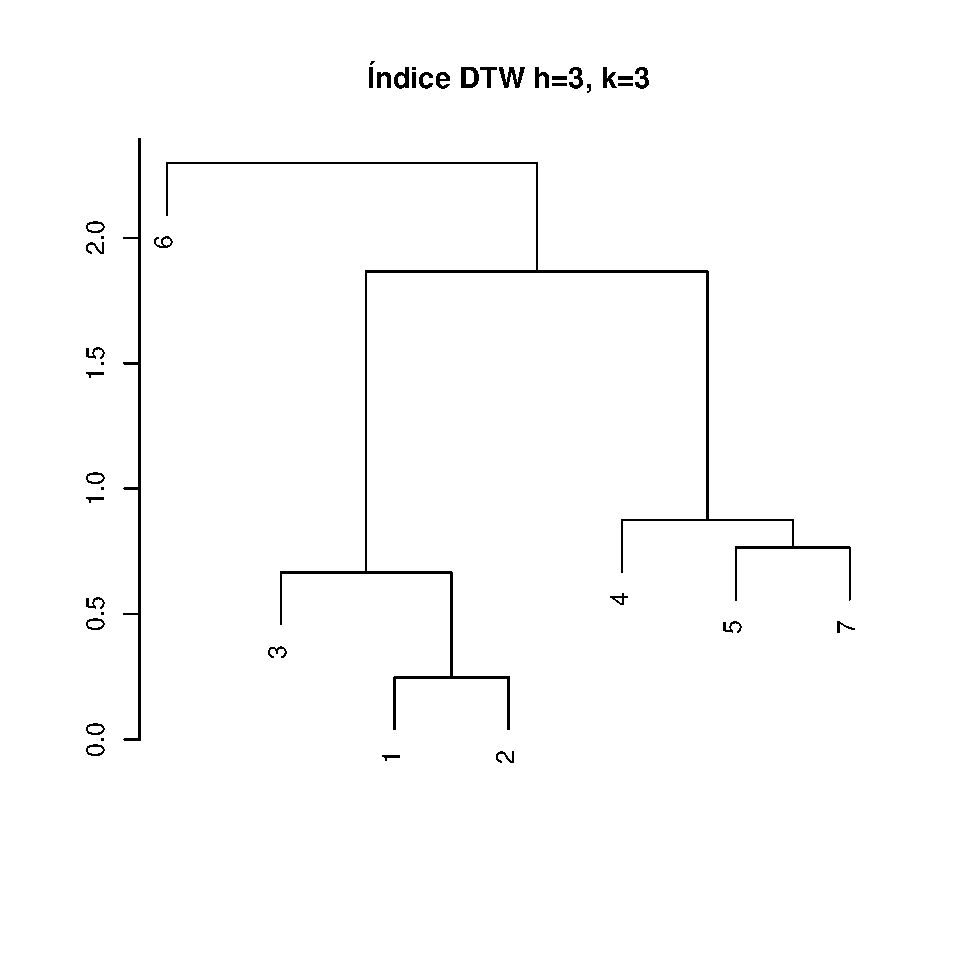
\includegraphics[height=4cm, width=4cm]{d233.eps}
       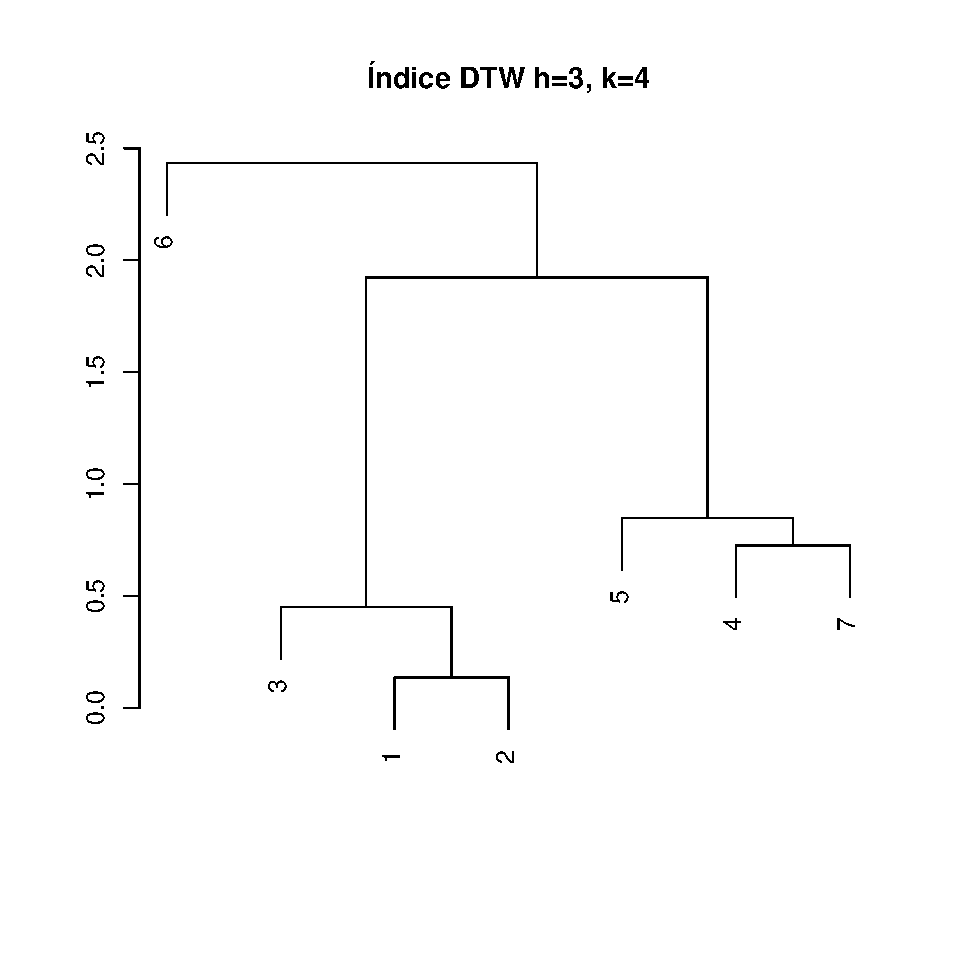
\includegraphics[height=4cm, width=4cm]{d234.eps}
\caption{Dendogramas \'Indice con $\delta_{DTW}$ con $h=3$, $k=1,2,3,4.$}
\label{caja}
\end{figure}

De igual manera sucede con $h=2$ y $k=1$ el algoritmo clasifica dos de las tres series. Con $h=2$, $h=3$ y $k=2,3$ el algoritmo vuelve agrupar las series se simularon.

\subsection{\'Indice de Disimilaridad Adaptativo con Distancia de Frech\'et}
Finalmente si se calcula el \'Indice de Disimilaridad con Distancia se Frech\'et, se pueden observar los siguientes resultados. El \'Indice calculado con $h=1,2$ y $k=1,2,3$ muestra algunas variaciones con los resultados esperados, ya que, el \'indice no logra percibir las diferencias entre las correlaciones. Por otra parte, con $h=3$ y  $k=1$, el \'Indice agrupa las series $X_t$, $Y_t$ y $W_t$.\\
De igual forma se puede apreciar que el \'Indice va agrupar mejor con altos valores de $h$ y $k$.


\begin{figure}[!htp]
       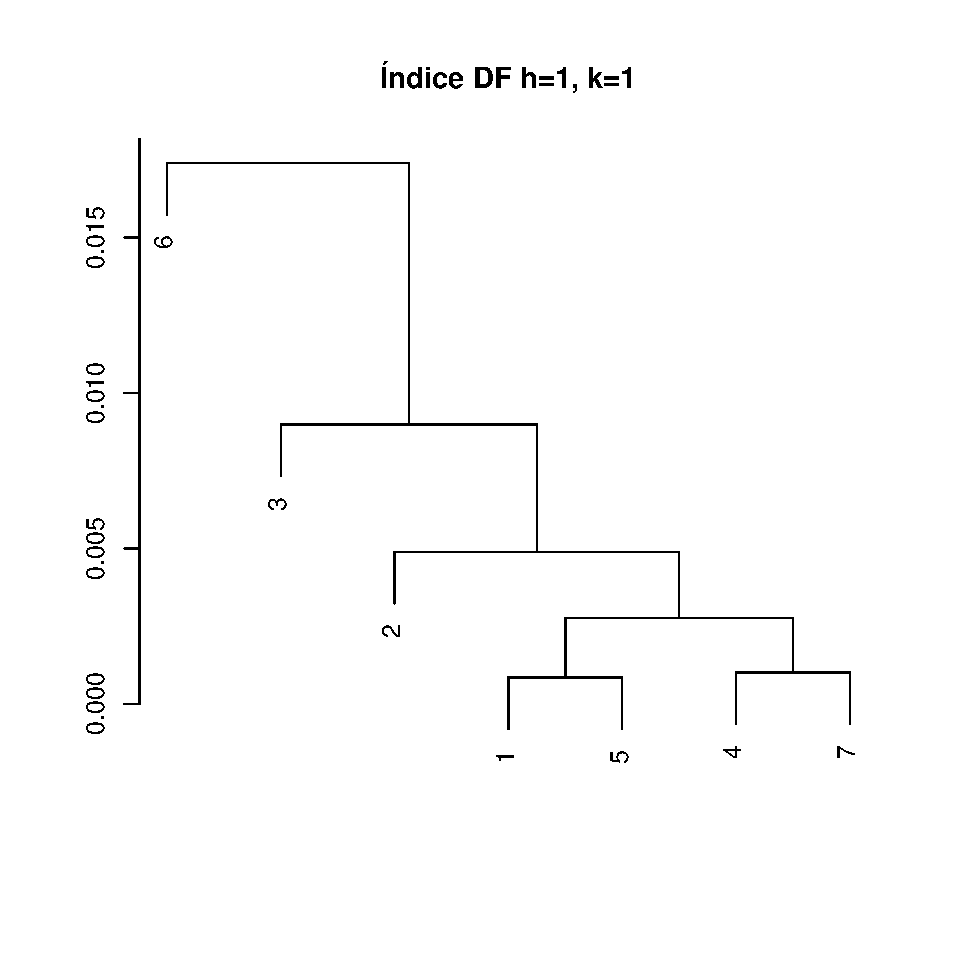
\includegraphics[height=4cm, width=4cm]{d311.eps}
       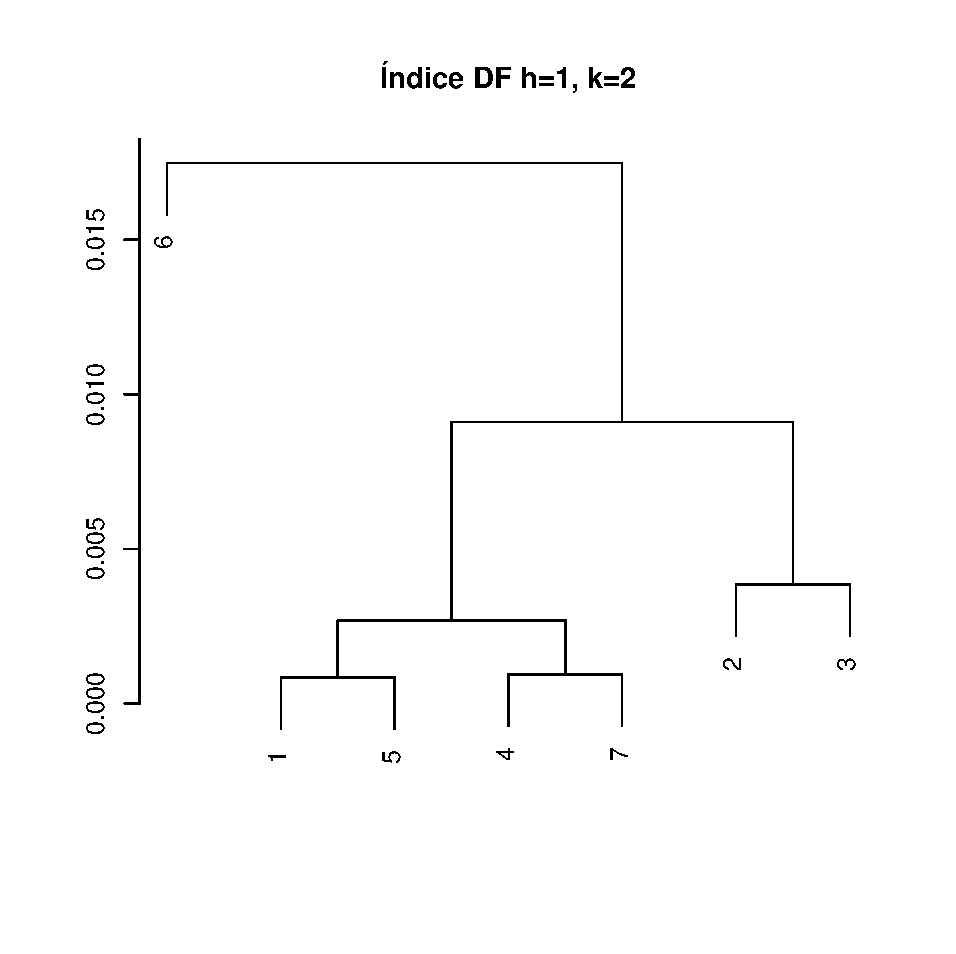
\includegraphics[height=4cm, width=4cm]{d312.eps}
       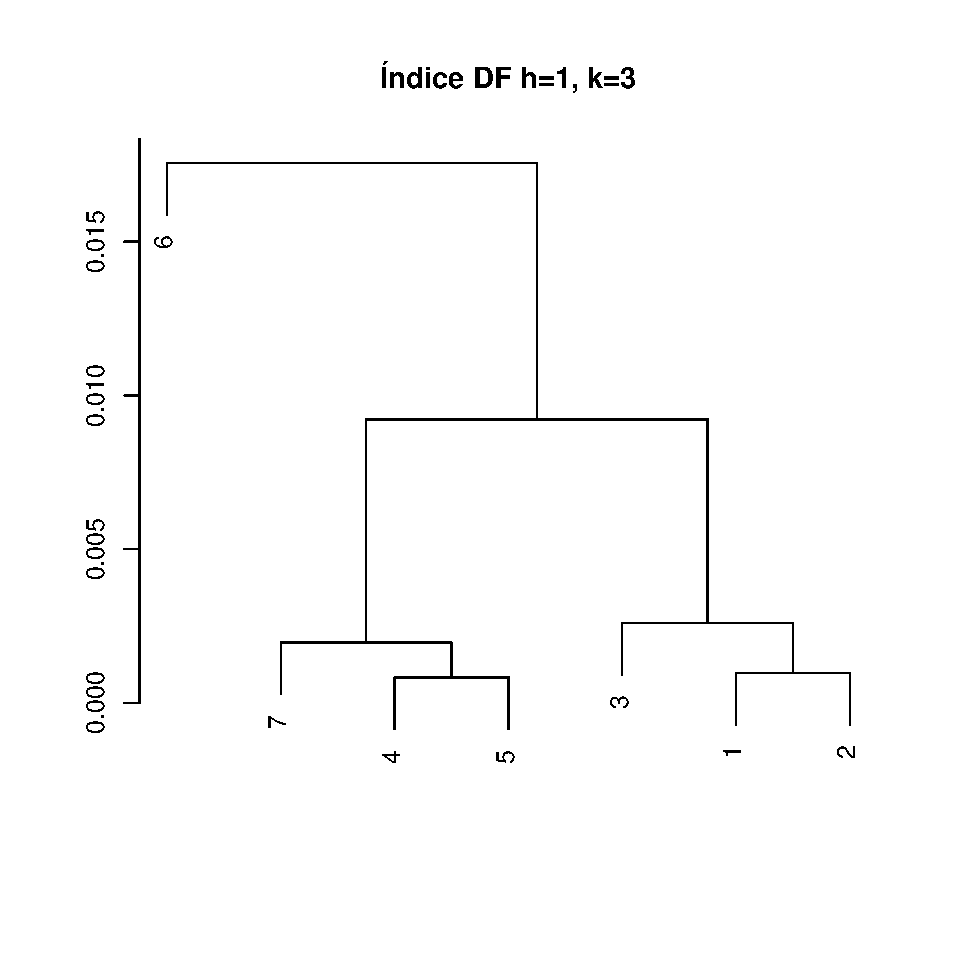
\includegraphics[height=4cm, width=4cm]{d313.eps}
       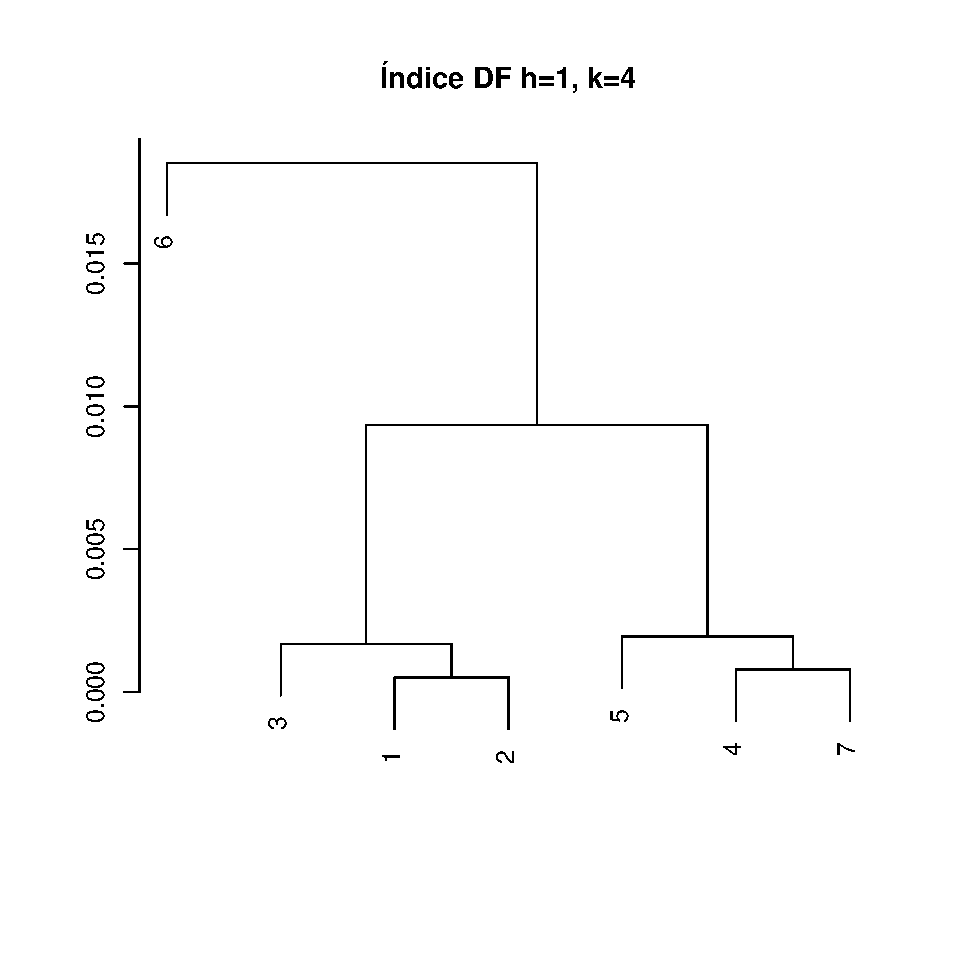
\includegraphics[height=4cm, width=4cm]{d314.eps}
\caption{Dendogramas \'Indice con $\delta_{F}$ con $h=1$, $k=1,2,3,4.$}
\label{caja}
\end{figure}


\begin{figure}[!htp]
       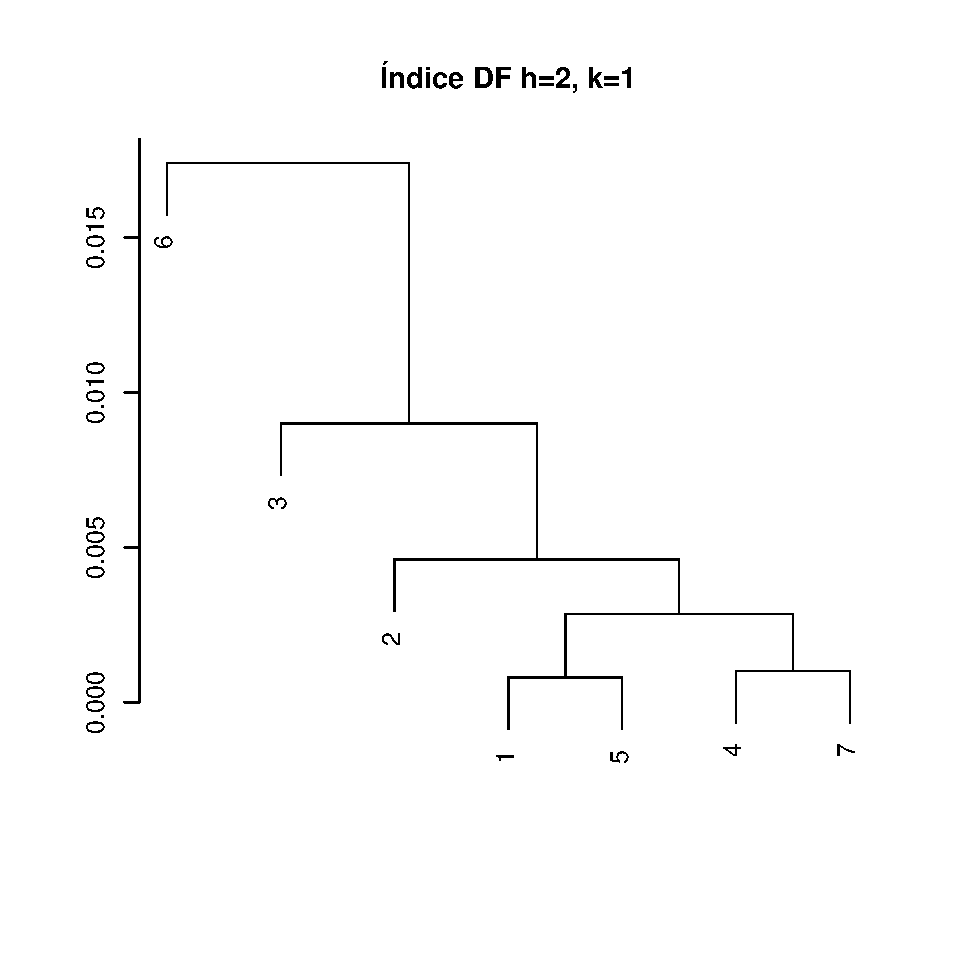
\includegraphics[height=4cm, width=4cm]{d321.eps}
       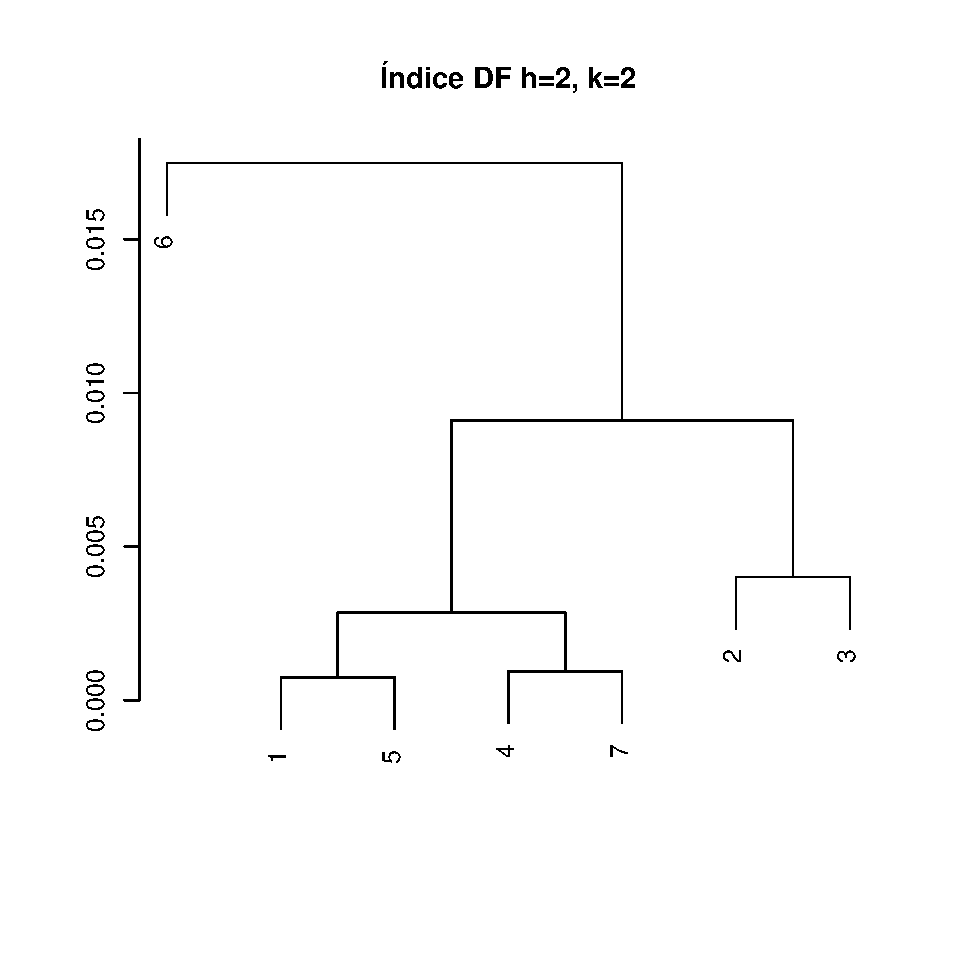
\includegraphics[height=4cm, width=4cm]{d322.eps}
       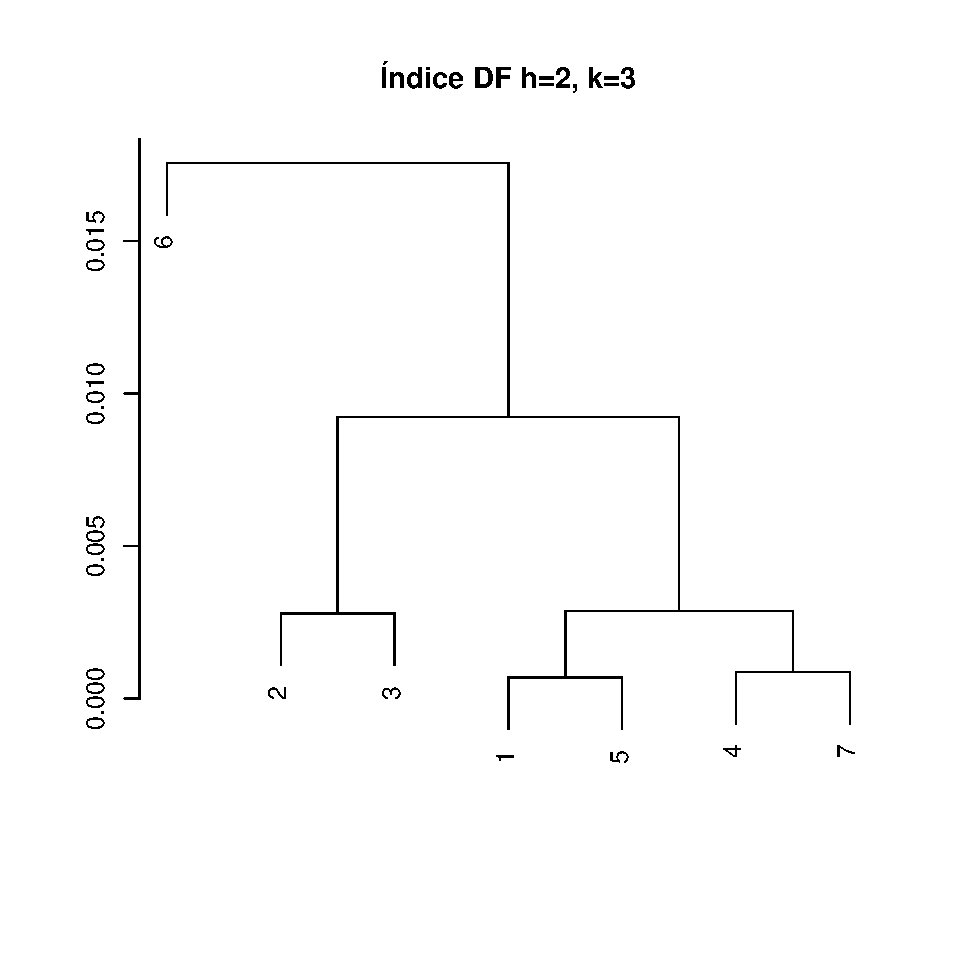
\includegraphics[height=4cm, width=4cm]{d323.eps}
       \includegraphics[height=4cm, width=4cm]{d324.eps}
\caption{Dendogramas \'Indice con $\delta_{F}$ con $h=2$, $k=1,2,3,4.$}
\label{caja}
\end{figure}

\begin{figure}[!htp]
       \includegraphics[height=4cm, width=4cm]{d331.eps}
       \includegraphics[height=4cm, width=4cm]{d332.eps}
       \includegraphics[height=4cm, width=4cm]{d333.eps}
       \includegraphics[height=4cm, width=4cm]{d334.eps}
\caption{Dendogramas \'Indice con $\delta_{F}$ con $h=3$, $k=1,2,3,4.$}
\label{caja}
\end{figure}

\newpage

\section{Conclusi\'on}
En los dendogramas se puede apreciar que el \'Indice de Disimilaridad con distancia euclidiana y DTW agrupa las series correlacionadas.

El \'Indice con la distancia de Frech\'et presenta una variaci\'on en la agrupaci\'on, ya que para valores altos de $h$ y $k$, los resultados son alcanzados.

La funci\'on de $k$, en el \'Indice de Disimilaridad modula la contribuci\'on del comovimiento respecto del comportamiento de los valores respecto a su cercan\'ia, esto se puede apreciar mejor cuando las distancias son poco sensibles, ya que para valores altos de $k$, la distancia convencional se ve afectada por una mayor contribuci\'on al comportamiento respecto del comovimiento, es decir, para valores de $k\geq 3$ la distancia convencional sera mas sensible a los cambios del comportamiento respecto de su comovimiento.

Es importante, calcular el \'Indice con distintos valores de h y k, para verificar y sacar conclusiones respecto de los grupos establecidos por esta nueva medida.

La simulaci\'on a demostrado que el \'Indice de Disimilaridad agrupa series temporales considerando su estructura de comovimiento y el comportamiento a su cercan\'ia, es decir, el \'Indice agrupa las series que est\'an fuertemente correlacionadas.

Se demostr\'o que las medidas convencionales ignoran la relaci\'on de interdependencia entre las medidas, ya que, son primordialmente basadas en la proximidad con relaci\'on a los valores.

%\section{Comparaci\'on de coeficientes anteriores para modelos ARMA.}

%\section{Compararci\'on de $D({X_{t}},{Y_{t}})$ con diferentes funciones.}


%\section{An\'alisis de la estacionalidad.}
%Por definir
%\section{Robustez de los coeficientes.}

% ------------------------------------------------------------------------

\def\baselinestretch{1}
\chapter{Aplicaci\'on a datos de AFP}
\def\baselinestretch{1.0}
\goodbreak
\section{Introducci\'on}
En las siguientes secciones se introducir\'a algunos conceptos
del Sistema de Pensiones, se hablar\'a de su funci\'on, sus g\'enesis y la reforma de Previsi\'on
 Social.

Estos conceptos nos ayudar\'an para entender y analizar 7 AFP distintas en el p\'eriodo de Enero 1990-Febrero 2004
en su rentabilidad mensual.

Las AFP en Estudio son:
\begin{itemize}
\item 1 = AFP CUPRUM, 2 = AFP HABITAT, 3 = AFP PROVIDA, 4 = AFP PLANVITAL, 5\-=\-AFP STA MARIA, 6 = AFP SUMMA, 7 = AFP MAGISTER.
\end{itemize}

El ahorro de los trabajadores ha sido fundamental para el crecimiento y
desarrollo econ\'omico de Chile, ya que ha sido mayoritariamente invertido en
actividades productivas o crediticias haciendo posible el acceso a financiamiento
de miles de chilenos, sea para comprar la casa propia o acceder a productos a los
que nunca antes tuvo oportunidad.

El sistema de AFP ha operado en estos 26 a\~nos bajo el principio de Giro \'Unico
o exclusivo lo cual ha resguardado los fondos previsionales de problemas como
las ventas atadas y los conflictos de inter\'es, que surgen cuando un administrador
de ahorros distribuye conjuntamente otros productos y adem\'as gestiona
simult\'aneamente dineros propios y de terceros.

\section{Sistema de AFP}

En noviembre de 1980 se public\'o el D.L. 3.500 que estableci\'o un nuevo sistema de pensiones de Vejez, Invalidez y Sobrevivencia, sobre la base del ahorro de los trabajadores y la capitalizaci\'on en cuentas individuales.

El nuevo Sistema de Pensiones incorpora el concepto de propiedad de los ahorros previsionales por parte de los trabajadores afiliados, enfatizando la estrecha correspondencia entre el esfuerzo de ahorro realizado a lo largo de la vida activa de una persona y los beneficios en pensiones de vejez, invalidez y sobrevivencia que \'esta recibe.

As\'i tambi\'en, se instaura la administraci\'on de los ahorros por empresas privadas (AFP), con giro \'unico y con el rol de otorgar beneficios y prestaciones previsionales. La normativa que regula a estas instituciones, adem\'as de la ley, es dictada por la Superintendencia de AFP, la que adem\'as fiscaliza el adecuado funcionamiento de estas sociedades.

El objetivo del Sistema de Pensiones es proveer ingresos de reemplazo para los trabajadores que dejan la vida activa o laboral y cubrir los riesgos de invalidez (total o parcial) y de muerte del trabajador (sobrevivencia), de manera de proteger al afiliado y a su grupo familiar.

Se basa en el ahorro y la Capitalizaci\'on Individual. Los trabajadores dependientes cotizan obligatoriamente en las AFP y los independientes lo hacen en forma voluntaria. Los trabajadores son due\~nos de su ahorro previsional y en ellos recae la responsabilidad de preocuparse de su pensi\'on, sin perjuicio que el Estado garantice pensiones m\'inimas.

Otorga libertad de elecci\'on a los afiliados. De este modo el trabajador puede elegir la administradora que gestione sus ahorros previsionales y cambiarse cuando lo desee, as\'i como la edad a la que quiere pensionarse (jubilaci\'on por vejez o anticipada) y la modalidad de pago de pensi\'on (retiro programado, renta vitalicia o retiro programado con renta vitalicia diferida). Asimismo, puede elegir el Tipo de Fondo en donde invertir sus ahorros.

Es uniforme en la aplicaci\'on de las normas para todos los afiliados y establece directa relaci\'on entre las contribuciones de los trabajadores y los beneficios obtenidos.

La administraci\'on es privada y est\'a a cargo de sociedades an\'onimas especializadas.

\section{Rentabilidad de los Fondos de Pensiones}

La rentabilidad de los fondos es un factor determinante en un sistema de
capitalizaci\'on y ahorro individual, donde el saldo acumulado durante la vida
activa del trabajador incidir\'a significativamente en el monto de las pensiones.
De esta forma, un punto porcentual de mayor ganancia anual puede elevar el
monto de la pensi\'on al cabo de 30 \'o 40 a\~nos de ahorro entre un 25 $\%$ y 30 $\%$.
Tras 26 a\~nos del sistema de pensiones la rentabilidad promedio real anual
alcanza a UF $+ 10$ $\%$, un resultado muy superior al $4$ a $5$ $\%$ de la rentabilidad
estimada como suficiente para financiar pensiones de reemplazo con una tasa
del orden del $70$ $\%$ del promedio de las remuneraciones.

\section{Contribuci\'on al Desarrollo Econ\'omico}

Los fondos de pensiones han hecho un aporte significativo al desarrollo
econ\'omico de Chile, otorgando, asimismo, acceso a amplios sectores de la
poblaci\'on a servicios financieros a los que nunca hab\'ian podido acceder.
Para un pa\'is en desarrollo como Chile, hoy econom\'ia emergente, disponer de
ahorro fue siempre un problema y una aspiraci\'on, ya que es sabido que el
c\'irculo virtuoso del progreso comienza con el ahorro y sigue con la inversi\'on y
el crecimiento. En la actualidad un 25 $\%$ del total de activos financieros
nacionales pertenece a los fondos de pensiones de los trabajadores, lo cual
constituye un aporte tangible al desarrollo econ\'omico.

El mercado de capitales chileno se ha expandido en forma significativa los
\'ultimos 26 a\~nos, progreso en el cual el ahorro de los fondos de pensiones ha
jugado un rol clave. Se han convertido en una fuente de financiamiento para el
Estado, para los bancos y para las empresas. El sistema de pensiones ha
introducido competencia en el mercado de capitales.

Casi el 100 $\%$ del financiamiento de letras hipotecarias para la vivienda y bonos
de bancos pertenece a los fondos de pensiones; tambi\'en un 45 $\%$ de los bonos
de empresas y un 55 $\%$ de los t\'itulos estatales.

\section{Antiguo Sistema Previsional}

Chile fue el primer pa\'is de Am\'erica Latina que cre\'o un Sistema de Seguridad Social, a comienzos del siglo XX. A lo largo de los a\~{n}os se fueron creando diversos reg\'imenes de pensiones diferenciados por el tipo de actividad o grupos ocupacionales con reglas y beneficios distintos.

Es as\'i como llegan a coexistir 52 $"\mbox{Cajas}"$ o Instituciones de Previsi\'on que operaban bajo el esquema de reparto. Esto significa que los aportes de los afiliados activos financiaban las pensiones de los pasivos y, por tanto, la subsistencia del Sistema estaba supeditada a la relaci\'on trabajador/pensionado existente en la poblaci\'on en cada momento del tiempo.

Durante los primeros a\~nos de existencia del sistema, la proporci\'on de trabajadores fue suficiente para financiar los beneficios de los pensionados. Sin embargo, los cambios demogr\'aficos, que fueron reflejando una permanente disminuci\'on de la natalidad y un aumento en las expectativas de vida revirtieron esta relaci\'on, provocando un fuerte desfinanciamiento del Sistema.

Mientras que en el a\~no 1955, por cada 12,2 trabajadores cotizantes hab\'ia 1 pensionado, en 1980 por cada 2,5 trabajadores cotizantes hab\'ia 1 pensionado. Es decir, s\'olo en 25 a\~nos el costo de los trabajadores cotizantes, se increment\'o casi 5 veces.

Un agravante del problema del financiamiento lo constituy\'o la fuerte evasi\'on previsional, ya que a trabajadores y empleadores les resultaba m\'as econ\'omico hacer imposiciones por el m\'inimo legal, preocup\'andose s\'olo de imponer por valores reales los \'ultimos a\~{n}os de la vida activa del trabajador, cuando las imposiciones eran consideradas para la jubilaci\'on. Esta situaci\'on obligaba al Estado a elevar las imposiciones lo que, a su vez, incentivaba una mayor evasi\'on previsional y as\'i sucesivamente.

A ellos se agrega que el Estado fue proclive a otorgar beneficios sin el adecuado financiamiento, lo que acentu\'o el problema rese\~{n}ado, ocasionando un d\'eficit fiscal creciente, equivalente a un 28 $\%$ del gasto en la d\'ecada 1970 - 1980.\\
El Antiguo Sistema se caracteriz\'o tambi\'en por su falta de equidad. Dado que no exist\'ia una relaci\'on directa entre los aportes de los trabajadores y
los beneficios percibidos, se apreciaban notables desigualdades entre los m\'ultiples grupos cubiertos. Esta situaci\'on se sustentaba
en la facultad del poder pol\'itico para definir qui\'en se beneficiaba y cu\'anto, quedando de manifiesto el otorgamiento de mayores
concesiones a los grupos que ejerc\'ian mayor presi\'on. En efecto, en  el a\~no 1965 (1), los obreros chilenos, que representaban el 70
$\%$ de los cotizantes y cuyos ingresos eran los m\'as bajos, percib\'ian en t\'erminos absolutos, pensiones equivalentes a la mitad de lo que
obten\'ian los empleados privados y a 1/14 de lo obtenido por los empleados p\'ublicos, los cuales eran grupos de mayores ingresos. Al mismo tiempo,
el aporte efectuado por estos trabajadores en el mismo per\'iodo (2), era equivalente a m\'as del doble
del que realizaban los empleados p\'ublicos y s\'olo un 10 $\%$ inferior al de los privados.

Desde hac\'ia mucho tiempo en nuestro pa\'is se presentaba la necesidad de introducir cambios al sistema de Seguridad Social. Ya en la d\'ecada del '60 se elaboraron diversos informes sobre las falencias del antiguo sistema de Seguridad Social Chileno en los que se propon\'ian cambios profundos.

El desfinanciamiento y la inequidad del esquema de reparto dieron origen a una reforma Previsional que cre\'o, mediante el D.L. 3.500 de 1980, un Nuevo Sistema de Pensiones basado en la Capitalizaci\'on Individual y administrado por entidades privadas denominadas Administradoras de Fondos de Pensiones (AFP). El Antiguo Sistema continu\'o funcionando, principalmente a trav\'es de un ente \'unico, denominado Instituto de Normalizaci\'on Previsional (INP), el cual fusion\'o a las principales Cajas de Previsi\'on.

El Estado se hizo responsable del financiamiento de las cotizaciones pagadas en el Antiguo Sistema por aquellas personas que se cambiaron al Nuevo Sistema. Ello se materializa a trav\'es de unos instrumentos financieros denominados Bonos de Reconocimiento, los cuales son representativos de dichos per\'iodos de cotizaciones y que el trabajador hace efectivo al instante de pensionarse o fallecer.

El Bono de Reconocimiento se reajusta de acuerdo a la variaci\'on de la inflaci\'on y devenga un inter\'es del 4 $\%$ real anual, el cual se capitaliza cada a\~{n}o.

\section{Efecto Manada}

Uno de los vicios que se le han imputado al sistema de AFP es que si todas no invirtieran en
los mismos activos, quiz\'as inyectar\'ian competencia al mercado por la v\'ia de ofrecer mejores
 retornos a los afiliados.

Es por eso que las distintas AFP invierten en acciones en las mismas empresas, revelando que la rentabilidad en las distintas  AFP son similares.
Este fen\'omeno se llama Efecto Manada.

\subsection{Contexto y consecuencias de la competencia en rentabilidad v\'ia ranking}

Para entender el contexto de esta competencia, es \'util tener en mente dos hechos.
Primero, las magnitudes de las diferencias en rentabilidad tienden a ser peque\~nas. De hecho, 10 puntos base de mayor o menor rentabilidad pueden hacer la diferencia entre el primero y el \'ultimo en el ranking en un a\~no determinado.

Segundo, hay extrema transparencia en las decisiones de inversi\'on. Las carteras de todos los fondos de pensiones son conocidas 10 d\'ias despu\'es de cerrado el mes. Si se imagina que una buena decisi\'on de inversi\'on es una especie de invento, entonces, en este caso, no habr\'ia un per\'iodo de protecci\'on o patente de uso; todos podr\'ian conocerlo y utilizarlo en forma gratuita pocos d\'ias despu\'es de haber sido creado.

Lo anterior, en forma absolutamente natural, genera incentivos a situarse muy cerca del benchmark (o vara de medida), que en este caso es la cartera de la competencia relevante, y a tomar decisiones en el margen, relativamente peque\~nas en magnitud. N\'otese que la cantidad de trabajo o estudio necesarios para tomar una buena decisi\'on de inversi\'on es la misma, independientemente de la magnitud de la decisi\'on de inversi\'on tomada. El riesgo pertinente pasa a ser el comercial, que consiste en quedar en una mala posici\'on en el ranking de rentabilidad. Una medida que refleja adecuadamente que el riesgo se mide en t\'erminos relativos es el llamado tracking error o variabilidad de la diferencia de retorno con el sistema. El fen\'omeno descrito genera el llamado efecto manada o herding (lo que, en todo caso, no es exclusividad del sistema adoptado en Chile, ya que, se da en casi toda la industria de administraci\'on de carteras).

Algo que s\'i es particular del caso chileno es que existe por ley una rentabilidad m\'inima que se calcula con respecto al promedio del sistema de AFP. Esta norma tiende a reafirmar el comportamiento descrito en el p\'arrafo anterior, pero es probable que incluso sin rentabilidad m\'inima la forma de competir fuera similar.

\section{Acciones favoritas de las AFP}

Seg\'un Econsult, en un Articulo publicado el 8 de Abril de 2008, en el Diario La Tercera, revisado el Mi\'ercoles 23 de Julio 2008,16:45 hrs, mostr\'o que Provida, apuesta m\'as que el resto en CMPC, donde mantiene una sobreesposici\'on de 1.81$\%$ respecto de la Industria. Su segunda apuesta m\'as fuerte comparativamente hablando es Endesa y AntarChile. La segunda AFP por fondo administrativo, Habitat, tiene como favorita a Telef\'onica CTC, seguida por Endesa y AntarChile.

Planvital e ING Santa Mar\'ia,por ejemplo, favorecen m\'as a Soquimich que el sistema como un todo, aunque luego sus preferencias difieran. Cuprum, por su parte, favorece a Colb\'un, las acciones de Telef\'onica CTC y a Masisa; y al cierre de Junio Summa Bansander mostraba una mayor inclinaci\'on por Endesa, D$\&$S y Copec.
\subsection{El m\'etodo de Encosult}
Enconsult sum\'o la inversi\'on directa de cada AFP en acciones mantenidas en los fondos A, B, C, D y E. Con ello pudo determinar el porcentaje del fondo invertido en cada t\'itulo y observar cu\'ales son las acciones que m\'as pesan en el.

Luego la consultora tomo esa exposici\'on total del sistema en una acci\'on y le resto la exposici\'on particular de cada AFP. El calculo se efectu\'o excluyendo del total a cada administradora seg\'un fuera el caso (sistema sin Bansander, luego sin Provida y as\'i). De esta forma pudo determinar en que porcentaje cada administradora esta sobre o bajo la media exposici\'on del sistema para cada inversion, evitando la distorsi\'on de que la AFP se compare en cierto modo consigo misma


\section{An\'alisis Descriptivo}

En esta secci\'on se har\'a un sondeo, para entender como se han comportado las 7 AFP, desde un punto de vista descriptivo.
En esta primera parte se realizar\'a un conteo para saber cuantas veces han estado primeras, es decir, con la mayor rentabilidad, en el caso que una AFP tiene la mayor rentabilidad se le asignara un valor 1 y al resto de las AFP 0, entonces, finalmente se sumara todos los casos para saber cuantas veces estuvo primera en rentabilidad, si hay mas de un empate, es decir, que mas de dos AFP tienen la mayor rentabilidad, se le asignaran a cada una el valor 1.

La siguiente tabla muestra los resultados obtenidos, para las AFP en estudio.

\begin{small}
\begin{center}
\begin{tabular}{|l|l|ll}
\cline{1-2}
AFP & CONTEO &  &  \\
\cline{1-2}
Cuprum & 35 &  &  \\
Habitat & 38 &  &  \\
Magister & 44 &  &  \\
Planvital & 26 &  &  \\
Provida & 37 &  &  \\
Sta Maria & 21 &  &  \\
Summa & 38 &  &  \\
\cline{1-2}
\end{tabular}
\end{center}
\end{small}

Se observa que la AFP que estuvo con mayor rentabilidad y esta primera con 44 veces dentro de este conteo es la AFP Magister, seguido de la AFP Provida que estuvo 37 veces primera y la AFP Cuprum con 35 veces.

\begin{figure}[!htp]
\centering
\fbox{ \includegraphics[height=4cm, width=6cm]{cajon.eps}}
\caption{Dispersi\'on de la rentabilidad de las AFP.}
\label{caja}
\end{figure}

Se puede observar que en gr\'afico de Caj\'on con bigotes, que hay datos que escapan a estos Cajones con bigotes. Adem\'as, las media son similares en todas las AFP. Acontinuaci\'on, se mostrara un sumario con algunas medidas descriptivas.


\begin{figure}[!htp]
\centering
\fbox{ \includegraphics[height=4cm, width=6cm]{s_afp.eps}}
\caption{7 Series durante 1990 - 2004.}
\label{caja}
\end{figure}

En el siguiente gr\'afico se muestra el comportamiento de la rentabilidad en el tiempo de las 7 AFP, si se observa el gr\'afico se puede apreciar una linea gruesa, este fen\'omeno se denomina efecto manada el cual se ha mencionado anteriormente y en consecuencia no se puede notar grandes diferencias. En la siguiente tabla se muestra un an\'alisis descriptivo por AFP.

\begin{center}
\begin{small}
\begin{tabular}{|l|l|l|l|l|l|l|l|}
\hline
\multicolumn{1}{|c|}{Estad\'isticos} & \multicolumn{1}{c|}{Cuprum} & \multicolumn{1}{c|}{Habitat} & \multicolumn{1}{c|}{Magister} & \multicolumn{1}{c|}{Planvital} & \multicolumn{1}{c|}{Provida} & \multicolumn{1}{c|}{ING Sta Mar\'ia} & \multicolumn{1}{c|}{Summa} \\
\hline
\multicolumn{1}{|c|}{Media} & \multicolumn{1}{c|}{0,83} & \multicolumn{1}{c|}{0,82} & \multicolumn{1}{c|}{0,84} & \multicolumn{1}{c|}{0,86} & \multicolumn{1}{c|}{0,78} & \multicolumn{1}{c|}{0,80} & \multicolumn{1}{c|}{0,85} \\
\multicolumn{1}{|c|}{Mediana} & \multicolumn{1}{c|}{0,81} & \multicolumn{1}{c|}{0,83} & \multicolumn{1}{c|}{0,86} & \multicolumn{1}{c|}{0,90} & \multicolumn{1}{c|}{0,80} & \multicolumn{1}{c|}{0,87} & \multicolumn{1}{c|}{0,90} \\
\multicolumn{1}{|c|}{Moda} & \multicolumn{1}{c|}{-1,10} & \multicolumn{1}{c|}{0,80} & \multicolumn{1}{c|}{-1,70} & \multicolumn{1}{c|}{1,60} & \multicolumn{1}{c|}{-1,60} & \multicolumn{1}{c|}{0,90} & \multicolumn{1}{c|}{-1,70} \\
\multicolumn{1}{|c|}{Desv Est} & \multicolumn{1}{c|}{1,82} & \multicolumn{1}{c|}{1,77} & \multicolumn{1}{c|}{1,92} & \multicolumn{1}{c|}{1,88} & \multicolumn{1}{c|}{1,68} & \multicolumn{1}{c|}{1,80} & \multicolumn{1}{c|}{1,82} \\
\multicolumn{1}{|c|}{Varianza } & \multicolumn{1}{c|}{3,31} & \multicolumn{1}{c|}{3,12} & \multicolumn{1}{c|}{3,70} & \multicolumn{1}{c|}{3,53} & \multicolumn{1}{c|}{2,82} & \multicolumn{1}{c|}{3,24} & \multicolumn{1}{c|}{3,33} \\
\multicolumn{1}{|c|}{Coef Var} & \multicolumn{1}{c|}{220,07} & \multicolumn{1}{c|}{215,03} & \multicolumn{1}{c|}{230,05} & \multicolumn{1}{c|}{219,74} & \multicolumn{1}{c|}{215,82} & \multicolumn{1}{c|}{224,85} & \multicolumn{1}{c|}{214,81} \\
\multicolumn{1}{|c|}{Rango} & \multicolumn{1}{c|}{14,60} & \multicolumn{1}{c|}{13,90} & \multicolumn{1}{c|}{14,20} & \multicolumn{1}{c|}{14,00} & \multicolumn{1}{c|}{13,00} & \multicolumn{1}{c|}{13,80} & \multicolumn{1}{c|}{13,90} \\
\multicolumn{1}{|c|}{M\'inimo} & \multicolumn{1}{c|}{-8,00} & \multicolumn{1}{c|}{-7,00} & \multicolumn{1}{c|}{-7,40} & \multicolumn{1}{c|}{-6,80} & \multicolumn{1}{c|}{-6,30} & \multicolumn{1}{c|}{-6,90} & \multicolumn{1}{c|}{-7,40} \\
\multicolumn{1}{|c|}{M\'aximo} & \multicolumn{1}{c|}{6,60} & \multicolumn{1}{c|}{6,90} & \multicolumn{1}{c|}{6,80} & \multicolumn{1}{c|}{7,20} & \multicolumn{1}{c|}{6,70} & \multicolumn{1}{c|}{6,90} & \multicolumn{1}{c|}{6,50} \\
\multicolumn{1}{|c|}{Cuenta} & \multicolumn{1}{c|}{170,00} & \multicolumn{1}{c|}{170,00} & \multicolumn{1}{c|}{170,00} & \multicolumn{1}{c|}{170,00} & \multicolumn{1}{c|}{170,00} & \multicolumn{1}{c|}{170,00} & \multicolumn{1}{c|}{170,00} \\
\hline
\end{tabular}
\end{small}
\end{center}

Si se observa la tabla se puede destacar que la rentabilidad media de Cuprum es de 0.8265, las rentabilidades extremas se pueden apreciar con un m\'inimo de -6.3 y un m\'aximo de 6.7. Adem\'as, se puede apreciar que en un 25$\%$ la rentabilidad llega a -0.175 y en el 75$\%$ llega a 1.7. Es claro, mencionar que para el resto de las AFP la interpretaci\'on es la misma.

M\'as adelante se estudiar\'an estas AFP, para representar, a trav\'es, de modelos param\'etricos y ver cual modelo puede representar mejor esta situaci\'on.

\section{Aplicaci\'on \'Indice de Comovimiento o Codispersi\'on}

Para el conjunto de 7 AFP, se calculara el \'Indice de Comovimiento para determinar en que grado comueven, los resultados son:

\paragraph{\'Indice de Comovimiento con $h=1$.}
\begin{center}
\begin{small}
\begin{tabular}{|l|l|l|l|l|l|l|lllllll}
\cline{1-7}
\multicolumn{1}{|c|}{$\rho(h=1)$} & \multicolumn{1}{c|}{Cuprum} & \multicolumn{1}{c|}{Habitat} & \multicolumn{1}{c|}{Provida} & \multicolumn{1}{c|}{Planvital} & \multicolumn{1}{c|}{Sta Mar\'ia} & \multicolumn{1}{c|}{Summa} &  &  &  &  &  &  &  \\
\cline{1-7}
\multicolumn{1}{|c|}{Habitat} & \multicolumn{1}{c|}{0,990} & \multicolumn{1}{c|}{} & \multicolumn{1}{c|}{} & \multicolumn{1}{c|}{} & \multicolumn{1}{c|}{} & \multicolumn{1}{c|}{} &  &  &  &  &  &  &  \\
\cline{1-7}
\multicolumn{1}{|c|}{Provida} & \multicolumn{1}{c|}{0,984} & \multicolumn{1}{c|}{0,982} & \multicolumn{1}{c|}{} & \multicolumn{1}{c|}{} & \multicolumn{1}{c|}{} & \multicolumn{1}{c|}{} &  &  &  &  &  &  &  \\
\cline{1-7}
\multicolumn{1}{|c|}{Planvital} & \multicolumn{1}{c|}{0,983} & \multicolumn{1}{c|}{0,987} & \multicolumn{1}{c|}{0,993} & \multicolumn{1}{c|}{} & \multicolumn{1}{c|}{} & \multicolumn{1}{c|}{} &  &  &  &  &  &  &  \\
\cline{1-7}
\multicolumn{1}{|c|}{Sta Maria} & \multicolumn{1}{c|}{0,982} & \multicolumn{1}{c|}{0,993} & \multicolumn{1}{c|}{0,970} & \multicolumn{1}{c|}{0,979} & \multicolumn{1}{c|}{} & \multicolumn{1}{c|}{} &  &  &  &  &  &  &  \\
\cline{1-7}
\multicolumn{1}{|c|}{Summa} & \multicolumn{1}{c|}{0,991} & \multicolumn{1}{c|}{0,995} & \multicolumn{1}{c|}{0,988} & \multicolumn{1}{c|}{0,992} & \multicolumn{1}{c|}{0,989} & \multicolumn{1}{c|}{} &  &  &  &  &  &  &  \\
\cline{1-7}
\multicolumn{1}{|c|}{Magister} & \multicolumn{1}{c|}{0,986} & \multicolumn{1}{c|}{0,985} & \multicolumn{1}{c|}{0,983} & \multicolumn{1}{c|}{0,986} & \multicolumn{1}{c|}{0,975} & \multicolumn{1}{c|}{0,987} &  &  &  &  &  &  &  \\
\cline{1-7}
\end{tabular}
\end{small}
\end{center}

Se puede observar que el comovimiento  entre las AFP es similar, es decir, estas comueven casi perfectamente en cualquier instante de tiempo.

\paragraph{\'Indice de Comovimiento con $h=2$.}

De igual forma si se calcula ahora con $h=2$, se puede apreciar los siguientes resultados:

\begin{center}
\begin{small}
\begin{tabular}{|l|l|l|l|l|l|l|lllllll}
\cline{1-7}
\multicolumn{1}{|c|}{$\rho(h=2)$} & \multicolumn{1}{c|}{Cuprum} & \multicolumn{1}{c|}{Habitat} & \multicolumn{1}{c|}{Provida} & \multicolumn{1}{c|}{Planvital} & \multicolumn{1}{c|}{Sta Mar\'ia} & \multicolumn{1}{c|}{Summa} &  &  &  &  &  &  &  \\
\cline{1-7}
\multicolumn{1}{|c|}{Habitat} & \multicolumn{1}{c|}{0,990} & \multicolumn{1}{c|}{} & \multicolumn{1}{c|}{} & \multicolumn{1}{c|}{} & \multicolumn{1}{c|}{} & \multicolumn{1}{c|}{} &  &  &  &  &  &  &  \\
\cline{1-7}
\multicolumn{1}{|c|}{Provida} & \multicolumn{1}{c|}{0,987} & \multicolumn{1}{c|}{0,985} & \multicolumn{1}{c|}{} & \multicolumn{1}{c|}{} & \multicolumn{1}{c|}{} & \multicolumn{1}{c|}{} &  &  &  &  &  &  &  \\
\cline{1-7}
\multicolumn{1}{|c|}{Planvital} & \multicolumn{1}{c|}{0,989} & \multicolumn{1}{c|}{0,987} & \multicolumn{1}{c|}{0,993} & \multicolumn{1}{c|}{} & \multicolumn{1}{c|}{} & \multicolumn{1}{c|}{} &  &  &  &  &  &  &  \\
\cline{1-7}
\multicolumn{1}{|c|}{Sta Maria} & \multicolumn{1}{c|}{0,983} & \multicolumn{1}{c|}{0,994} & \multicolumn{1}{c|}{0,970} & \multicolumn{1}{c|}{0,979} & \multicolumn{1}{c|}{} & \multicolumn{1}{c|}{} &  &  &  &  &  &  &  \\
\cline{1-7}
\multicolumn{1}{|c|}{Summa} & \multicolumn{1}{c|}{0,992} & \multicolumn{1}{c|}{0,995} & \multicolumn{1}{c|}{0,988} & \multicolumn{1}{c|}{0,992} & \multicolumn{1}{c|}{0,989} & \multicolumn{1}{c|}{} &  &  &  &  &  &  &  \\
\cline{1-7}
\multicolumn{1}{|c|}{Magister} & \multicolumn{1}{c|}{0,990} & \multicolumn{1}{c|}{0,985} & \multicolumn{1}{c|}{0,983} & \multicolumn{1}{c|}{0,986} & \multicolumn{1}{c|}{0,975} & \multicolumn{1}{c|}{0,987} &  &  &  &  &  &  &  \\
\cline{1-7}
\end{tabular}
\end{small}
\end{center}

Los valores est\'an cercanos a $1$, es decir, que las series se mueven conjuntamente iguales en cualquier periodo de tiempo $[t_i,t_{i+2}]$ En este caso los valores son similares a la tabla anterior.

\paragraph{\'Indice de Comovimiento con $h=3$.}

Ahora con $h=3$, se pueden apreciar valores similares.

\begin{center}
\begin{small}
\begin{tabular}{|l|l|l|l|l|l|l|lllllll}
\cline{1-7}
\multicolumn{1}{|c|}{$\rho(h=3)$} & \multicolumn{1}{c|}{Cuprum} & \multicolumn{1}{c|}{Habitat} & \multicolumn{1}{c|}{Provida} & \multicolumn{1}{c|}{Planvital} & \multicolumn{1}{c|}{Sta Mar\'ia} & \multicolumn{1}{c|}{Summa} &  &  &  &  &  &  &  \\
\cline{1-7}
\multicolumn{1}{|c|}{Habitat} & \multicolumn{1}{c|}{0,988} & \multicolumn{1}{c|}{} & \multicolumn{1}{c|}{} & \multicolumn{1}{c|}{} & \multicolumn{1}{c|}{} & \multicolumn{1}{c|}{} &  &  &  &  &  &  &  \\
\cline{1-7}
\multicolumn{1}{|c|}{Provida} & \multicolumn{1}{c|}{0,986} & \multicolumn{1}{c|}{0,987} & \multicolumn{1}{c|}{} & \multicolumn{1}{c|}{} & \multicolumn{1}{c|}{} & \multicolumn{1}{c|}{} &  &  &  &  &  &  &  \\
\cline{1-7}
\multicolumn{1}{|c|}{Planvital} & \multicolumn{1}{c|}{0,988} & \multicolumn{1}{c|}{0,987} & \multicolumn{1}{c|}{0,993} & \multicolumn{1}{c|}{} & \multicolumn{1}{c|}{} & \multicolumn{1}{c|}{} &  &  &  &  &  &  &  \\
\cline{1-7}
\multicolumn{1}{|c|}{Sta Maria} & \multicolumn{1}{c|}{0,981} & \multicolumn{1}{c|}{0,994} & \multicolumn{1}{c|}{0,970} & \multicolumn{1}{c|}{0,979} & \multicolumn{1}{c|}{} & \multicolumn{1}{c|}{} &  &  &  &  &  &  &  \\
\cline{1-7}
\multicolumn{1}{|c|}{Summa} & \multicolumn{1}{c|}{0,990} & \multicolumn{1}{c|}{0,995} & \multicolumn{1}{c|}{0,988} & \multicolumn{1}{c|}{0,992} & \multicolumn{1}{c|}{0,989} & \multicolumn{1}{c|}{} &  &  &  &  &  &  &  \\
\cline{1-7}
\multicolumn{1}{|c|}{Magister} & \multicolumn{1}{c|}{0,983} & \multicolumn{1}{c|}{0,985} & \multicolumn{1}{c|}{0,983} & \multicolumn{1}{c|}{0,986} & \multicolumn{1}{c|}{0,975} & \multicolumn{1}{c|}{0,987} &  &  &  &  &  &  &  \\
\cline{1-7}
\end{tabular}
\end{small}
\end{center}

\paragraph{\'Indice de Comovimiento con $h=4$.}

 Finalmente con $h=4$, las diferencias entre valores no son significativa por simple inspecci\'on.

\begin{center}
\begin{small}
\begin{tabular}{|l|l|l|l|l|l|l|lllllll}
\cline{1-7}
\multicolumn{1}{|c|}{$\rho(h=4)$} & \multicolumn{1}{c|}{Cuprum} & \multicolumn{1}{c|}{Habitat} & \multicolumn{1}{c|}{Provida} & \multicolumn{1}{c|}{Planvital} & \multicolumn{1}{c|}{Sta Mar\'ia} & \multicolumn{1}{c|}{Summa} &  &  &  &  &  &  &  \\
\cline{1-7}
\multicolumn{1}{|c|}{Habitat} & \multicolumn{1}{c|}{0,990} & \multicolumn{1}{c|}{} & \multicolumn{1}{c|}{} & \multicolumn{1}{c|}{} & \multicolumn{1}{c|}{} & \multicolumn{1}{c|}{} &  &  &  &  &  &  &  \\
\cline{1-7}
\multicolumn{1}{|c|}{Provida} & \multicolumn{1}{c|}{0,986} & \multicolumn{1}{c|}{0,987} & \multicolumn{1}{c|}{} & \multicolumn{1}{c|}{} & \multicolumn{1}{c|}{} & \multicolumn{1}{c|}{} &  &  &  &  &  &  &  \\
\cline{1-7}
\multicolumn{1}{|c|}{Planvital} & \multicolumn{1}{c|}{0,989} & \multicolumn{1}{c|}{0,989} & \multicolumn{1}{c|}{0,993} & \multicolumn{1}{c|}{} & \multicolumn{1}{c|}{} & \multicolumn{1}{c|}{} &  &  &  &  &  &  &  \\
\cline{1-7}
\multicolumn{1}{|c|}{Sta Maria} & \multicolumn{1}{c|}{0,982} & \multicolumn{1}{c|}{0,993} & \multicolumn{1}{c|}{0,970} & \multicolumn{1}{c|}{0,979} & \multicolumn{1}{c|}{} & \multicolumn{1}{c|}{} &  &  &  &  &  &  &  \\
\cline{1-7}
\multicolumn{1}{|c|}{Summa} & \multicolumn{1}{c|}{0,992} & \multicolumn{1}{c|}{0,995} & \multicolumn{1}{c|}{0,988} & \multicolumn{1}{c|}{0,992} & \multicolumn{1}{c|}{0,989} & \multicolumn{1}{c|}{} &  &  &  &  &  &  &  \\
\cline{1-7}
\multicolumn{1}{|c|}{Magister} & \multicolumn{1}{c|}{0,990} & \multicolumn{1}{c|}{0,985} & \multicolumn{1}{c|}{0,983} & \multicolumn{1}{c|}{0,986} & \multicolumn{1}{c|}{0,975} & \multicolumn{1}{c|}{0,987} &  &  &  &  &  &  &  \\
\cline{1-7}
\end{tabular}
\end{small}
\end{center}

Este alto grado de comovimiento, se puede deber a que las AFP bajo el fen\'omeno de efecto manada, comuevan casi perfectamente en cualquier instante de tiempo $[t_i,t_{i+h}]$.

\section{Modelamiento}

Como se mencion\'o anteriormente, se estudiar\'a la estacionariedad y el comportamiento de la rentabilidad. Para poder modelar esta situaci\'on se usar\'a las definiciones de series de tiempo mencionadas anteriormente y se estudiara como se comportan respecto al \'indice o coeficiente de Codispersi\'on para ver cual es su grado de comovimiento.

Por otra parte, se aplicar\'a el \'indice de disimilaridad, para clasificar las AFP respecto a su rentabilidad y considerando la estructura de correlaci\'on temporal, esto ayudar\'a a responder los objetivos de este Proyecto de T\'itulo.

Las hip\'otesis que contempla este Proyecto de T\'itulo, es que las series que se estudiaran son estacionarias.

Para analizar la estacionalidad, hay varios aspectos que se tienen que considerar, proponer transformaciones que ayudar\'an a estabilizar la varianza unas propuestas son $\log{x}$, $\sqrt{x}$, $\frac{1}{x}$ y desplazar la serie en $c$ por nombrar algunas. Otra alternativa es, a trav\'es, de la estructura de correlaci\'on temporal que en este caso es la funci\'on de autocorrelaci\'on (ACF) y funci\'on de autocorrelaci\'on parcial (Partial ACF), estas estructuras ayudaran a proponer un modelo que se pueda ajustar mejor a esta situaci\'on.

Para esto, existen valores que nos ayudan a comparar cuales de los modelos se ajusta mejor, como es el criterio Akaike (AIC), donde el AIC m\'as peque\~{n}o evidencia un mejor ajuste. Observando las series por separado, como muestra la siguiente figura.


\begin{figure}[!ht]
\begin{center}
\centering
  \includegraphics[height=4cm, width=4cm]{afp1.eps}
  \includegraphics[height=4cm, width=4cm]{afp2.eps}
  \includegraphics[height=4cm, width=4cm]{afp3.eps}
  \includegraphics[height=4cm, width=4cm]{afp4.eps}\\
  \includegraphics[height=4cm, width=4cm]{afp5.eps}
  \includegraphics[height=4cm, width=4cm]{afp6.eps}
  \includegraphics[height=4cm, width=4cm]{afp7.eps}
   \caption{Rentabilidad AFP.}
\label{caja}
\end{center}
\end{figure}

En estos Gr\'aficos, se puede apreciar el comportamiento similar de las 7 AFP. Donde se puede observar que en todas las AFP, en el per\'iodo de Noviembre 1997 y en Enero, Junio y Septiembre de 1998, las AFP muestran sus ca\'idas mas significativas. Con Septiembre de 1998 la ca\'ida mas importante de estas, este  dato at\'ipico podr\'ia afectar la modelaci\'on en sus par\'ametros o quiz\'as a validar el supuesto de normalidad.

Como las AFP muestran rentabilidades con valores negativos y adem\'as, se puede notar que la varianza de la rentabilidad de las AFP no es constante, proponer una tansformaci\'on que nos ayude a homogenizar la varianza y dejar las series estacionarias, se tienen que considerar estos valores. Por lo general,para homogenizar la varianza se ocupan $\sqrt(x)$ y $\log(x)$, pero como existen valores negativos, habr\'ian casos indeterminados,es por eso que se trasladara esta serie en 10 unidades, un n\'umero un poco mayor al de los valores extremos que es -7.4, para as\'i tener valores positivos y homogenizar la serie con el $\log(x)$. Acontinuaci\'on, se muestran las series transformadas:

\begin{figure}[!ht]
\begin{center}
\centering
  \includegraphics[height=4cm, width=4cm]{afptr1.eps}
  \includegraphics[height=4cm, width=4cm]{afptr2.eps}
  \includegraphics[height=4cm, width=4cm]{afptr3.eps}
  \includegraphics[height=4cm, width=4cm]{afptr4.eps}\\
  \includegraphics[height=4cm, width=4cm]{afptr5.eps}
  \includegraphics[height=4cm, width=4cm]{afptr6.eps}
  \includegraphics[height=4cm, width=4cm]{afptr7.eps}
   \caption{Transformaci\'on AFP.}
\label{caja}
\end{center}
\end{figure}

En la Figura 4.4 se puede apreciar, que si bien la serie esta m\'as estacionaria, a\'un se puede apreciar que la ca\'ida de septiembre 1998 afecta, al intentar homogenizar la varianza.

Luego de analizar la estacionariedad de las AFP, propondremos un modelo que represente esta situaci\'on. Si consideramos las funciones ACF  y Partial ACF, los resultados son los siguientes.

\begin{figure}[!ht]
\centering
  \includegraphics[height=4cm, width=4cm]{acf1.eps}
  \includegraphics[height=4cm, width=4cm]{acf2.eps}
  \includegraphics[height=4cm, width=4cm]{acf3.eps}
  \includegraphics[height=4cm, width=4cm]{acf4.eps}
\label{caja}
\end{figure}

\begin{figure}[!ht]
\centering
  \includegraphics[height=4cm, width=4cm]{acf5.eps}
  \includegraphics[height=4cm, width=4cm]{acf6.eps}
  \includegraphics[height=4cm, width=4cm]{acf7.eps}
   \caption{Funci\'on de Autocorrelaci\'on AFP.}
\label{caja}
\end{figure}

Se observa que la memoria del proceso  es de un retardo. Como se presento anteriormente en la Figura 4.5 de la rentabilidad de las AFP se puede observar una cierta estacionalidad, propia de los modelos de media m\'ovil. Ahora bien, se analizar\'a que sucede con la funci\'on de autocorrelaci\'on parcial

\begin{figure}[!ht]
\begin{center}
\centering
  \includegraphics[height=4cm, width=4cm]{pacf1.eps}
  \includegraphics[height=4cm, width=4cm]{pacf2.eps}
  \includegraphics[height=4cm, width=4cm]{pacf3.eps}
  \includegraphics[height=4cm, width=4cm]{pacf4.eps}\\
  \includegraphics[height=4cm, width=4cm]{pacf5.eps}
  \includegraphics[height=4cm, width=4cm]{pacf6.eps}
  \includegraphics[height=4cm, width=4cm]{pacf7.eps}
   \caption{Funci\'on de Autocorrelaci\'on Parcial AFP.}
\label{caja}
\end{center}
\end{figure}
En base a la Figura 4.6 se pueden proponer algunos modelos a priori, para representar la rentabilidad de las AFP.\\
La parte autoregresiva contribuye en 2 lag o retardos, Por otra parte, la estructura de media mov\'il contribuye con 1 lag o retardo. Acontinuaci\'on algunas propuestas de modelos para esta situaci\'on.
\begin{center}
\begin{tabular}{|l|l|ll}
\cline{1-2}
Modelos Propuestos & AIC &  &  \\
\cline{1-2}
ARMA(1,1) & -60.71 &  &  \\
ARMA(2,1) & -58.73 &  &  \\
AR(1) & -60.98 &  &  \\
MA(1) & -61.84 &  &  \\
\cline{1-2}
\end{tabular}
\end{center}

Si se observa el AIC de los modelos propuestos, el modelo que minimiza la varianza de los residuos es el modelo de media mov\'il MA(1). Las AFP son modelados a trav\'es de  MA(1), desde aqu\'i, se puede analizar supuesto de normalidad.

\section{Estimaci\'on de par\'ametros MA(1) y an\'alisis de residuos}
En esta seccion se presentaran las estiamciones de los coeficiente de los modelos MA(1) para cada una de las AFP.
\paragraph{Estimaci\'on de par\'ametros AFP Cuprum}
\begin{center}
\begin{tabular}{|l|l|l|}
\hline
\multicolumn{1}{|c|}{Par\'ametros} & \multicolumn{1}{c|}{MA(1)} & \multicolumn{1}{c|}{Intercepto} \\
\hline
\multicolumn{1}{|c|}{Coeficiente} & \multicolumn{1}{c|}{-0,9684} & \multicolumn{1}{c|}{-1,00E-04} \\
\hline
\multicolumn{1}{|c|}{s.e} & \multicolumn{1}{c|}{0,0356} & \multicolumn{1}{c|}{3,00E-04} \\
\hline
\multicolumn{1}{|c|}{$\hat{\sigma}^{2}$} & \multicolumn{1}{c|}{Log Ver} & \multicolumn{1}{c|}{AIC} \\
\hline
\multicolumn{1}{|c|}{0,01031} & \multicolumn{1}{c|}{145,37} & \multicolumn{1}{c|}{-284,75} \\
\hline
\end{tabular}
\end{center}
\paragraph{Estimaci\'on de par\'ametros AFP Habitat}
\begin{center}
\begin{tabular}{|l|l|l|}
\hline
\multicolumn{1}{|c|}{Par\'ametros} & \multicolumn{1}{c|}{MA(1)} & \multicolumn{1}{c|}{Intercepto} \\
\hline
\multicolumn{1}{|c|}{Coeficiente} & \multicolumn{1}{c|}{-0,9675} & \multicolumn{1}{c|}{-1,00E-04} \\
\hline
\multicolumn{1}{|c|}{s.e} & \multicolumn{1}{c|}{0,0371} & \multicolumn{1}{c|}{3,00E-04} \\
\hline
\multicolumn{1}{|c|}{$\hat{\sigma}^{2}$} & \multicolumn{1}{c|}{Log Ver} & \multicolumn{1}{c|}{AIC} \\
\hline
\multicolumn{1}{|c|}{0,0084} & \multicolumn{1}{c|}{162,69} & \multicolumn{1}{c|}{-319,39} \\
\hline
\end{tabular}
\end{center}
\paragraph{Estimaci\'on de par\'ametros AFP Provida}
\begin{center}
\begin{tabular}{|l|l|l|}
\hline
\multicolumn{1}{|c|}{Par\'ametros} & \multicolumn{1}{c|}{MA(1)} & \multicolumn{1}{c|}{Intercepto} \\
\hline
\multicolumn{1}{|c|}{Coeficiente} & \multicolumn{1}{c|}{-0,9629} & \multicolumn{1}{c|}{-1,00E-04} \\
\hline
\multicolumn{1}{|c|}{s.e} & \multicolumn{1}{c|}{0,0379} & \multicolumn{1}{c|}{2,00E-04} \\
\hline
\multicolumn{1}{|c|}{$\hat{\sigma}^{2}$} & \multicolumn{1}{c|}{Log Ver} & \multicolumn{1}{c|}{AIC} \\
\hline
\multicolumn{1}{|c|}{0,003579} & \multicolumn{1}{c|}{234,85} & \multicolumn{1}{c|}{-463,71} \\
\hline
\end{tabular}
\end{center}
\paragraph{Estimaci\'on de par\'ametros AFP Planvital}
\begin{center}
\begin{tabular}{|l|l|l|}
\hline
\multicolumn{1}{|c|}{Par\'ametros} & \multicolumn{1}{c|}{MA(1)} & \multicolumn{1}{c|}{Intercepto} \\
\hline
\multicolumn{1}{|c|}{Coeficiente} & \multicolumn{1}{c|}{-0,9621} & \multicolumn{1}{c|}{-2,00E-04} \\
\hline
\multicolumn{1}{|c|}{s.e} & \multicolumn{1}{c|}{0,0346} & \multicolumn{1}{c|}{3,00E-04} \\
\hline
\multicolumn{1}{|c|}{$\hat{\sigma}^{2}$} & \multicolumn{1}{c|}{Log Ver} & \multicolumn{1}{c|}{AIC} \\
\hline
\multicolumn{1}{|c|}{0,009118} & \multicolumn{1}{c|}{155,84} & \multicolumn{1}{c|}{-305,69} \\
\hline
\end{tabular}
\end{center}
\paragraph{Estimaci\'on de par\'ametros AFP Sta. Mar\'ia}
\begin{center}
\begin{tabular}{|l|l|l|}
\hline
\multicolumn{1}{|c|}{Par\'ametros} & \multicolumn{1}{c|}{MA(1)} & \multicolumn{1}{c|}{Intercepto} \\
\hline
\multicolumn{1}{|c|}{Coeficiente} & \multicolumn{1}{c|}{-0,96} & \multicolumn{1}{c|}{4,20E-03} \\
\hline
\multicolumn{1}{|c|}{s.e} & \multicolumn{1}{c|}{0,0437} & \multicolumn{1}{c|}{6,40E-03} \\
\hline
\multicolumn{1}{|c|}{$\hat{\sigma}^{2}$} & \multicolumn{1}{c|}{Log Ver} & \multicolumn{1}{c|}{AIC} \\
\hline
\multicolumn{1}{|c|}{3,128} & \multicolumn{1}{c|}{-337,44} & \multicolumn{1}{c|}{680,88} \\
\hline
\end{tabular}
\end{center}
\paragraph{Estimaci\'on de par\'ametros AFP Summa}
\begin{center}
\begin{tabular}{|l|l|l|}
\hline
\multicolumn{1}{|c|}{Par\'ametros} & \multicolumn{1}{c|}{MA(1)} & \multicolumn{1}{c|}{Intercepto} \\
\hline
\multicolumn{1}{|c|}{Coeficiente} & \multicolumn{1}{c|}{0,2786} & \multicolumn{1}{c|}{1,27E+00} \\
\hline
\multicolumn{1}{|c|}{s.e} & \multicolumn{1}{c|}{0,0805} & \multicolumn{1}{c|}{7,10E-03} \\
\hline
\multicolumn{1}{|c|}{$\hat{\sigma}^{2}$} & \multicolumn{1}{c|}{Log Ver} & \multicolumn{1}{c|}{AIC} \\
\hline
\multicolumn{1}{|c|}{0,005291} & \multicolumn{1}{c|}{204,29} & \multicolumn{1}{c|}{-402,58} \\
\hline
\end{tabular}
\end{center}
\paragraph{Estimaci\'on de par\'ametros AFP Magister}

\begin{center}
\begin{tabular}{|l|l|l|}
\hline
\multicolumn{1}{|c|}{Par\'ametros} & \multicolumn{1}{c|}{MA(1)} & \multicolumn{1}{c|}{Intercepto} \\
\hline
\multicolumn{1}{|c|}{Coeficiente} & \multicolumn{1}{c|}{-0,9626} & \multicolumn{1}{c|}{-1,00E-04} \\
\hline
\multicolumn{1}{|c|}{s.e} & \multicolumn{1}{c|}{0,0346} & \multicolumn{1}{c|}{3,00E-04} \\
\hline
\multicolumn{1}{|c|}{$\hat{\sigma}^{2}$} & \multicolumn{1}{c|}{Log Ver} & \multicolumn{1}{c|}{AIC} \\
\hline
\multicolumn{1}{|c|}{0,005998} & \multicolumn{1}{c|}{191,22} & \multicolumn{1}{c|}{-376,44} \\
\hline
\end{tabular}
\end{center}

\paragraph{Test de bondad de ajuste}

En esta parte se presentar\'a la verificaci\'on del supuesto de normalidad de los residuos para cada modelo a trav\'es del test de Shapiro Wilks, presentando su estad\'istica y el valor-$p$.
\begin{center}
\begin{tabular}{|l|l|l|}
\hline
\multicolumn{1}{|c|}{AFP} & \multicolumn{1}{c|}{W} & \multicolumn{1}{c|}{p-valor} \\
\hline
\multicolumn{1}{|c|}{Cuprum} & \multicolumn{1}{c|}{0,7983} & \multicolumn{1}{c|}{0} \\
\hline
\multicolumn{1}{|c|}{Habitat} & \multicolumn{1}{c|}{0,8817} & \multicolumn{1}{c|}{0} \\
\hline
\multicolumn{1}{|c|}{Provida} & \multicolumn{1}{c|}{0,8946} & \multicolumn{1}{c|}{0} \\
\hline
\multicolumn{1}{|c|}{Planvital} & \multicolumn{1}{c|}{0,8924} & \multicolumn{1}{c|}{0} \\
\hline
\multicolumn{1}{|c|}{Sta. Maria} & \multicolumn{1}{c|}{0,9773} & \multicolumn{1}{c|}{0,007089} \\
\hline
\multicolumn{1}{|c|}{Summa} & \multicolumn{1}{c|}{0,9095} & \multicolumn{1}{c|}{0} \\
\hline
\multicolumn{1}{|c|}{Magister} & \multicolumn{1}{c|}{0,8946} & \multicolumn{1}{c|}{0} \\
\hline
\end{tabular}
\end{center}

A continuaci\'on se presentan histogramas de los residuos de las 7 AFP.

\begin{figure}[!htp]
\begin{center}
\centering
  \includegraphics[height=4cm, width=4cm]{grafico1.eps}
  \includegraphics[height=4cm, width=4cm]{grafico2.eps}
  \includegraphics[height=4cm, width=4cm]{grafico3.eps}
  \includegraphics[height=4cm, width=4cm]{grafico4.eps}
  \includegraphics[height=4cm, width=4cm]{grafico5.eps}
  \includegraphics[height=4cm, width=4cm]{grafico6.eps}
  \includegraphics[height=4cm, width=4cm]{grafico7.eps}
   \caption{Histograma de los residuos AFP.}
\label{caja}
\end{center}
\end{figure}

\section{An\'alisis de Cluster}
En esta secci\'on se implementar\'a el algoritmo de clasificaci\'on para series temporales con el \'Indice de Disimilaridad Adaptativo para distancias convencionales.

Para entender mejor los dendogramas se han definido los siguientes valores que estar\'an re\-fe\-ren\-cian\-do a las AFP.

\begin{itemize}
\item 1 = AFP CUPRUM, 2 = AFP HABITAT, 3 = AFP PROVIDA, 4 = AFP PLANVITAL, 5 = AFP STA MARIA, 6 = AFP SUMMA y 7 = AFP MAGISTER
\end{itemize}

Aplicando el algoritmo de clasificaci\'on para series temporales con las distancias convencionales se tiene que:

\begin{figure}[!htp]
\begin{center}
\centering
  \includegraphics[height=4cm, width=4cm]{den_dist_euc.eps}
  \includegraphics[height=4cm, width=4cm]{den_dist_dfr.eps}
  \includegraphics[height=4cm, width=4cm]{den_dist_dtw.eps}
   \caption{Dendogramas.}
\label{caja}
\end{center}
\end{figure}

En estos gr\'aficos se puede apreciar los distintos grupos con las tres distancias:
La distancia euclidiana forma dos grupos:

\begin{tabular}{|l|l|}
\hline
Grupo 1 & Grupo 2 \\
\hline
(2)(6)(5) & (3)(4)(3)(1)(7) \\
\hline
\end{tabular}
\\
\\
La distancia de Frech\'et agrupa las AFP:

\begin{tabular}{|l|l|}
\hline
Grupo 1 & Grupo 2 \\
\hline
(3)(4)(1) & (2)(7)(5)(6) \\
\hline
\end{tabular}

La distancia DTW agrupa las AFP:

\begin{tabular}{|l|l|}
\hline
Grupo 1 & Grupo 2 \\
\hline
(3)(4) & (2)(6)(3)(1)(7) \\
\hline
\end{tabular}

\subsection{Camino Distorsionado entre AFP}
La siguiente Figura muestran la alineaci\'on entre las AFP, se presentan algunas combinaciones de la AFP CUPRUM con el resto de las AFP, y se destaca presencia de una perfecta alineaci\'on, es decir, las unidades ex\-pe\-ri\-men\-ta\-les entre par de punto son similares.

\begin{figure}[!htp]
\begin{center}
\centering
  \includegraphics[height=3cm, width=4cm]{c_d1.eps}
  \includegraphics[height=3cm, width=4cm]{c_d2.eps}
  \includegraphics[height=3cm, width=4cm]{c_d3.eps}\\
  \includegraphics[height=3cm, width=4cm]{c_d4.eps}
  \includegraphics[height=3cm, width=4cm]{c_d5.eps}
  \includegraphics[height=3cm, width=4cm]{c_d6.eps}
   \caption{Alineamiento entre AFP.}
\label{caja}
\end{center}
\end{figure}

Esta gran similitud se debe al efecto manada, el cual ha sido detectado usando el \'Indice de Comovimiento.

\subsection{Aplicaci\'on \'Indice de Disimilaridad con Distancia Euclidiana}

Si se calcula el \'Indice usando la distancia euclidiana y se aplica el algoritmo de clasificaci\'on se puede observar que de acuerdo a la definici\'on esta calcula y re\'une las AFP que est\'an m\'as cerca respecto a cada una de las unidades experimentales, este algoritmo se calculo con $h=1,2$ y $k=1,2,3$.

\begin{figure}[!htp]
\begin{center}
\centering
  \includegraphics[height=3cm, width=4cm]{i_euc_h_1_k_1.eps}
  \includegraphics[height=3cm, width=4cm]{i_euc_h_1_k_2.eps}
  \includegraphics[height=3cm, width=4cm]{i_euc_h_1_k_3.eps}\\
  \includegraphics[height=3cm, width=4cm]{i_euc_h_2_k_1.eps}
  \includegraphics[height=3cm, width=4cm]{i_euc_h_2_k_2.eps}
  \includegraphics[height=3cm, width=4cm]{i_euc_h_2_k_3.eps}
   \caption{Dendogramas de las AFP con \'Indice usando $\delta_{E}$ con $h=1,2$ y $k=1,2,3.$}
\label{caja}
\end{center}
\end{figure}

Los dendogramas con el \'Indice Adaptativo no muestra cambios respecto de la distancia eu\-cli\-dia\-na.

\subsection{Aplicaci\'on \'Indice de Disimilaridad con Distancia Frech\'et}

Este \'Indice agrupa las AFP considerando las distancias m\'as peque\~nas dentro de las diferencias m\'aximas de cada unidad experimental. Se puede apreciar que este \'Indice presenta algunas variaciones cuando$h=2$, esta variaci\'on de agrupaci\'on es solo el intercambio de prioridad del algoritmo de Clasificaci\'on.

\begin{figure}[!htp]
\centering
  \includegraphics[height=3cm, width=4cm]{i_df_h_1_k_1.eps}
  \includegraphics[height=3cm, width=4cm]{i_df_h_1_k_2.eps}
  \includegraphics[height=3cm, width=4cm]{i_df_h_1_k_3.eps}\\
  \includegraphics[height=3cm, width=4cm]{i_df_h_2_k_1.eps}
  \includegraphics[height=3cm, width=4cm]{i_df_h_2_k_2.eps}
  \includegraphics[height=3cm, width=4cm]{i_df_h_2_k_3.eps}
  \caption{Dendogramas de las  AFP  con \'Indice usando $\delta_{F}$ con h=1,2 y k=1,2,3}
\label{caja}
\end{figure}

En general este \'Indice no presenta, cambios respecto de su distancia convencional.

\subsection{Aplicaci\'on \'Indice de Disimilaridad con Distancia DTW}

Con el \'Indice de Disimilaridad adaptativo usando la distancia $\delta_{DTW}$, agrupa las AFP que est\'an m\'as alineadas.
Este \'Indice no presenta cambios respecto de su medida convencional.

\begin{figure}[!htp]
\centering
  \includegraphics[height=3cm, width=4cm]{i_dtw_h_1_k_1.eps}
  \includegraphics[height=3cm, width=4cm]{i_dtw_h_1_k_2.eps}
  \includegraphics[height=3cm, width=4cm]{i_dtw_h_1_k_3.eps}\\
  \includegraphics[height=3cm, width=4cm]{i_dtw_h_2_k_1.eps}
  \includegraphics[height=3cm, width=4cm]{i_dtw_h_2_k_2.eps}
  \includegraphics[height=3cm, width=4cm]{i_dtw_h_2_k_3.eps}
  \caption{Dendogramas de las AFP con \'Indice usando $\delta_{DTW}$ con h=1,2 y k=1,2,3}
\label{caja}
\end{figure}
\newpage
\section{Conclusi\'on}
En este cap\'itulo se pudo conocer como se comportan las AFP, el an\'alisis descriptivo muestra evidencia de que las AFP tienen rentabilidad promedio bastante parecidas, as\'i como en la desviaci\'on est\'andar. Seguidamente, se ha propuesto un modelo que mejor representa el comportamiento de la rentabilidad, basados en la informaci\'on del AIC que son los modelos de media m\'ovil de orden 1, es decir MA(1). Adem\'as, se han calculado los par\'ametros para cada una de las 7 AFP y se analiz\'o los residuos, donde la normalidad se ve afectada fuertemente por la crisis asi\'atica en los a\~nos de 1997-1998.

En en an\'alisis de cluster, en \'Indice de Disimilaridad Adaptativo ha presentado pocos cambios respecto de sus medidas convencionales, dado la fuerte similitud de las AFP y en consecuencia, no ha podido detectar diferencias tanto en su nivel de comovimiento y de cercan\'ia.


\chapter{Conclusiones}
\def\baselinestretch{1.0}
\medskip
Las ventajas que tiene el \'Indice de Comovimiento es la capacidad de capturar la informaci\'on respecto del comovimiento conjunto de las series, esto se ha podido observar en el sistema Chileno de AFP, donde deja en evidencia que la rentabilidad en el tiempo de las 7 AFP en estudio tienen el mismo comportamiento, lo interesante de cuantificar este fen\'omeno es tambi\'en, buscar las posibles causas de este fen\'omeno. Actualmente el modelo del sistema de pensiones ha sido cuestionado debido, a la poca competencia por abrir e investigar en otros mercados burs\'atiles, ya que las AFP en estudios invierten en las mismas acciones. Otra causa a considerar es la crisis ec\'onomica mundial, donde se ha creado un ambiente de desconfianza entre los inversionistas, esto motiva a que las personas sean m\'as conservadoras en las inversiones.

Tambi\'en se ha estudiado el \'Indice de Disimilaridad y se ha presentado la definici\'on y las propiedades de algunas medidas convencionales ampliamente usadas.

Se ha estudiado el comportamiento de las AFP y se ha podido determinar que esta rentabilidad es representada por modelos de media m\'ovil MA(1), esto motiva el estudio de una representaci\'on param\'etrica asociada a esta medida de similaridad.

En la simulaci\'on se ha demostrado que las medidas convencionales $\delta_{E}$, $\delta_{M}$, $\delta_{F}$ y $\delta_{DTW}$ ignoran la relaci\'on de interdependencia entre las series y son primordialmente basadas en la proximidad con relaci\'on a los valores. Para evitar esta limitaci\'on, se ha estudiado el \'Indice de Disimilaridad que tiene en cuenta la proximidad con relaci\'on al comportamiento y con relaci\'on a los valores.

Esta medida de Disimilaridad es una funci\'on del \'Indice de Comovimiento y se ha mostrado una medida de similaridad bastante razonable en relaci\'on a los valores, la Disimilaridad propuesta es definida como una funci\'on adaptable de afinaci\'on que balancea la proximidad con relaci\'on a los valores y la proximidad con relaci\'on al comportamiento.

En la simulaci\'on se ha estudiado la contribuci\'on del comportamiento y componentes de valores para el \'Indice de Disimilaridad y se compar\'o con las medidas convencionales.

Las desventajas del \'Indice de Comovimiento es que para series no estacionarias a\'un no se ha estudiado un estimador adecuado. Adem\'as, la presencia de outliers afecta fuertemente la estimaci\'on de su comovimiento, lo que provocar\'ia sesgo en las estimaciones dando conclusiones err\'oneas.

Por otra parte el \'Indice de Comovimiento o Codispersi\'on tiene su extensi\'on para procesos espaciales intr\'insicamente estacionarios, como son los procesos autoregresivos, media m\'ovil y ARMA espacial.

En este proyecto de t\'itulo, no se a estudiado una version no par\'ametrica, debido a que este coeficiente esta basado el estimador de momentos de $\rho_{X,Y}$, pero con esto, no se dice que no se pueda implementar un coeficiente de codispersi\'on no param\'etrico, pero esto motivar\'ia otro estudio.

Las aplicaciones que tiene el coeficiente de codispersi\'on se pueden ver en Vallejos. (2008) \textit{Similarity Coefficients for Spatial or Temporal Sequences.}

En trabajos posteriores se podr\'ia estudiar la robustez de Coeficiente de Codispersi\'on, para estar seguro que los distintos grados de comovimiento est\'en bien representados y evitar sobre estimaciones de la codispersi\'on. Adem\'as, estudiar la estacionariedad de las series, proponer y estudiar en Coeficiente de Codispersi\'on para series no estacionarias. Otro aspecto a considerar es la compararci\'on de el \'Indice de Disimilaridad Adaptativo $D({X_{t}},{Y_{t}})$ con diferentes funciones que ayuden a detectar y modular peque\~{n}as diferencias en el comportamiento de las series.






\nonumchapter{Bibliograf\'ia}
\def\baselinestretch{1.0}
\medskip


\begin{itemize}
\item $[1]$ Rukhin and Vallejos. (2008) Assessing the Asociation Between Two Spatial or Temporal Sequences. Journal of Applied Statistics. P\'ag.1-2.5-7.  P\'agina web www.deuv.cl/vallejos
\item $[2]$ Vallejos. (2008) Similarity Coefficients for Spatial or Temporal Sequences. Journal of A\-ppli\-ed Statistics. P\'ag.1-4
\item $[3]$ A.D. Choaukria and P.N. Nagabbhushan. (2007) Adaptive dissimilarity index for mea\-su\-ring time series proximity. Springer-Verlag. P\'ag. 1-17.
\item $[4]$ T. Warren Liao. (2005) Clustering of time data- a survey. The Journal of de Pattern Recognition Society. P\'ag.1-6
\item $[5]$ Dallas E.Johnson. (1998) M\'etodos Multivariados Aplicados Al An\'alisis de Datos. International Thompson Editores. M\'exico. P\'ag.323-329.
\item $[6]$ E. Keogh and A. Ratanamahatana. (2004) Exact indexing of dynamic time warping. Springer-Verlag. P\'ag. 1-4
\item $[7]$ T. Eiter and H. Mannila. (1994). Computing Discrete Frechet Distance. Technischen Universit$\ddot{a}$t Wien. P\'ag. 1-5
\item $[8]$ S. Salvador and P. Chan (2006) FastDTW: Toward Accurate Dynamic Time Warping in Linear Time and Space. Institute of Technology. Melbourne. P\'ag. 1-2.
\item $[9]$ E. Walker (2006). Aspectos Financieros del Sistema de AFP. Universidad Cat\'olica de Chile. P\'ag.1-3.
\item $[10]$ Memoria Corporativa (2007). Asociacion Gremial de Administradores de Fondos de Pensiones. P\'ag. 4-6.7-11.
\item $[11]$ Ngai Hang Chan, Time Series: Applications to Finance, Willey Series in probability and Statistics.(2002). P\'ag. 39-54.
\item $[12]$ Dag Tj$\phi$stheim. A measure of association for spatial variables. Biometrika (1978). P\'ag. 109-114.
\end{itemize}


\nonumchapter{Anexo}
\def\baselinestretch{1.0}
\medskip

\section*{Rutinas para R}
\begin{verbatim}
#########################################################################
library(dtw)

##########################Base de datos AFP################################
X<-matrix(0,ncol=7,nrow=170)
X<-read.table(file='C:/Users/Juan Carlos Herrera/
Documents/Seminario de Tesis/Datos afp.txt')
X<-as.matrix(X)
ts.plot(X,gpars=list(xlab="Tiempo", ylab="",main="Rentabilidad AFP" ))
boxplot(as.data.frame(X))
##################################################################################

X<-read.table(file='C:/Users/Juan Carlos Herrera/Documents
/Seminario de Tesis/Datos_CUPRUM.txt')
X<-as.matrix(X)

########################Vectorizamos###################################################
l<-dim(X)[1]
v1<-matrix(0,nrow=l,ncol=1)
v2<-matrix(0,nrow=l,ncol=1)
v3<-matrix(0,nrow=l,ncol=1)
v4<-matrix(0,nrow=l,ncol=1)
v5<-matrix(0,nrow=l,ncol=1)
v6<-matrix(0,nrow=l,ncol=1)
v7<-matrix(0,nrow=l,ncol=1)

for(i in 1:l)
  {
   v1[i]<-X[i,1]
   v2[i]<-X[i,2]
   v3[i]<-X[i,3]
   v4[i]<-X[i,4]
   v5[i]<-X[i,5]
   v6[i]<-X[i,6]
   v7[i]<-X[i,7]
   }
##############################################################
#####Algunas funciones para calcular distancia######################
########Distancia Euclidiana#####################################
de<-function(a,b)
{
n<-length(a)
s<-0
vec<-matrix(0,n,1)
for(i in 1:n)
 {
   vec[i]<-(a[i]-b[i])^2
   s<-sqrt(sum(vec))
 }
s
}
################Distancia de Frechet##########################################
d<-function(a,b)
{
c<-abs(a-b)
c
}

x<-c(1.4,2.3,3.09,4.3,1.3)
y<-c(6.02,7.1,9.01,0,1,6,2.1,3.3)

df<-function(x,y)
{
p<-length(x)
q<-length(y)
ca<-matrix(-1,nrow=p,ncol=q)
c<-matrix(0,nrow=p,ncol=q)
ca[1,1]<-d(x[1],y[1])
k<-1
l<-1
s<-0
for(i in 2:p)
{
ca[i,k]<-max(ca[i-1,k],d(x[i],y[k]))
}
for(j in 2:q)
{
ca[l,j]<-max(ca[l,j-1],d(x[l],y[j]))
}
 for(i in 2:p)
 {
  for(j in 2:q)
  {
   ca[i,j]<-min(max(ca[i-1,j],ca[i-1,j-1],ca[i,j-1]),d(x[i],y[j]))
  }
 }
  for(i in 1:p)
  {
   for(j in 1:q)
   {
   if(ca[i,j]>-1)
   {
   a<-ca[i,j]
   a
   }
  else
  {
  s<-100000
  s
  }
}
}
a
}

###########################Coeficiente de Codispersion#################

cod<-function(a,b,h)
{
n<-length(a)
m<-length(b)
vec<-matrix(0,n,1)
vec1<-matrix(0,n,1)
vec2<-matrix(0,n,1)
s1<-0
s2<-0
s3<-0
r<-0
  for(i in 1:n-h)
     {
      vec[i]=(a[i+h]-a[i])*(b[i+h]-b[i])
      vec1[i]=(a[i+h]-a[i])^2
      vec2[i]=(b[i+h]-b[i])^2
      s1<-sum(vec)
      s2<-sqrt(sum(vec1))
      s3<-sqrt(sum(vec2))
     }
r<-(s1/(s2*s3))
r
}
##########################Indice de disimilaridad######################
D<-function(a,b,h,k)
{
l<-length(a)
p1<-cod(a,b,h)
p2<-de(a,b)/(l)
v<-(2/(1+exp(p1*k)))
f<-(v*p2)
f
}

########################################################################

D1<-function(a,b,h,k)
{
l<-length(a)
p1<-cod(a,b,h)
p2<-dtw(a,b)$distance/(l)
v<-(2/(1+exp(k*p1)))
f<-(v*p2)
f
}

################################################################################

D2<-function(a,b,h,k)
{
l<-length(a)
p1<-cod(a,b,h)
p2<-df(a,b)/l
v<-(2/(1+exp(k*p1)))
f<-(v*p2)
f
}

#######################Funcion de disimilaridad que transforma matriz de
distancia en objeto dist##############################################
#h=h1
#t=h2
#k=k

cl<-function(A,B,C,V,E,F,G,h,k)
{
a<-D(A,B,h,k)
b<-D(A,C,h,k)
y<-D(A,V,h,k)
d<-D(A,E,h,k)
m<-D(A,F,h,k)
l<-D(A,G,h,k)
e<-D(B,C,h,k)
g<-D(B,V,h,k)
h<-D(B,E,h,k)
o<-D(B,F,h,k)
p<-D(B,G,h,k)
q<-D(C,V,h,k)
z<-D(C,E,h,k)
t<-D(C,F,h,k)
u<-D(C,G,h,k)
n<-D(V,E,h,k)
r<-D(V,F,h,k)
s<-D(V,G,h,k)
w<-D(E,F,h,k)
f1<-D(E,G,h,k)
w1<-D(F,G,h,k)

A1<-matrix(c(0,a,b,y,d,m,l),7,1)
B2<-matrix(c(a,0,e,g,h,o,p),7,1)
C3<-matrix(c(b,e,0,q,z,t,u),7,1)
D4<-matrix(c(y,g,q,0,n,r,s),7,1)
P5<-matrix(c(d,h,z,n,0,w,f1),7,1)
P6<-matrix(c(m,o,t,r,w,0,w1),7,1)
P7<-matrix(c(l,p,u,s,f1,w1,0),7,1)


MD<-matrix(cbind(A1,B2,C3,D4,P5,P6,P7),7,7)
md<-as.dist(MD)
md
}

############################################################

cl1<-function(A,B,C,V,E,F,G,h,k)
{
a<-D1(A,B,h,k)
b<-D1(A,C,h,k)
y<-D1(A,V,h,k)
d<-D1(A,E,h,k)
m<-D1(A,F,h,k)
l<-D1(A,G,h,k)
e<-D1(B,C,h,k)
g<-D1(B,V,h,k)
h<-D1(B,E,h,k)
o<-D1(B,F,h,k)
p<-D1(B,G,h,k)
q<-D1(C,V,h,k)
z<-D1(C,E,h,k)
t<-D1(C,F,h,k)
u<-D1(C,G,h,k)
n<-D1(V,E,h,k)
r<-D1(V,F,h,k)
s<-D1(V,G,h,k)
w<-D1(E,F,h,k)
f1<-D1(E,G,h,k)
w1<-D1(F,G,h,k)

A1<-matrix(c(0,a,b,y,d,m,l),7,1)
B2<-matrix(c(a,0,e,g,h,o,p),7,1)
C3<-matrix(c(b,e,0,q,z,t,u),7,1)
D4<-matrix(c(y,g,q,0,n,r,s),7,1)
P5<-matrix(c(d,h,z,n,0,w,f1),7,1)
P6<-matrix(c(m,o,t,r,w,0,w1),7,1)
P7<-matrix(c(l,p,u,s,f1,w1,0),7,1)


MD<-matrix(cbind(A1,B2,C3,D4,P5,P6,P7),7,7)
md<-as.dist(MD)
md
}

####################################################################################

cl2<-function(A,B,C,V,E,F,G,h,k)
{
a<-D2(A,B,h,k)
b<-D2(A,C,h,k)
y<-D2(A,V,h,k)
d<-D2(A,E,h,k)
m<-D2(A,F,h,k)
l<-D2(A,G,h,k)
e<-D2(B,C,h,k)
g<-D2(B,V,h,k)
h<-D2(B,E,h,k)
o<-D2(B,F,h,k)
p<-D2(B,G,h,k)
q<-D2(C,V,h,k)
z<-D2(C,E,h,k)
t<-D2(C,F,h,k)
u<-D2(C,G,h,k)
n<-D2(V,E,h,k)
r<-D2(V,F,h,k)
s<-D2(V,G,h,k)
w<-D2(E,F,h,k)
f1<-D2(E,G,h,k)
w1<-D2(F,G,h,k)

A1<-matrix(c(0,a,b,y,d,m,l),7,1)
B2<-matrix(c(a,0,e,g,h,o,p),7,1)
C3<-matrix(c(b,e,0,q,z,t,u),7,1)
D4<-matrix(c(y,g,q,0,n,r,s),7,1)
P5<-matrix(c(d,h,z,n,0,w,f1),7,1)
P6<-matrix(c(m,o,t,r,w,0,w1),7,1)
P7<-matrix(c(l,p,u,s,f1,w1,0),7,1)


MD<-matrix(cbind(A1,B2,C3,D4,P5,P6,P7),7,7)
md<-as.dist(MD)
md
}

###########################Funcion que transforma matriz de distancia
en objeto dist para DE##################
m_d<-function(A,B,C,V,E,F,G)
{
a<-de(A,B)
b<-de(A,C)
y<-de(A,V)
d<-de(A,E)
m<-de(A,F)
l<-de(A,G)
e<-de(B,C)
g<-de(B,V)
h<-de(B,E)
o<-de(B,F)
p<-de(B,G)
q<-de(C,V)
z<-de(C,E)
t<-de(C,F)
u<-de(C,G)
n<-de(V,E)
r<-de(V,F)
s<-de(V,G)
w<-de(E,F)
f1<-de(E,G)
w1<-de(F,G)

A1<-matrix(c(0,a,b,y,d,m,l),7,1)
B2<-matrix(c(a,0,e,g,h,o,p),7,1)
C3<-matrix(c(b,e,0,q,z,t,u),7,1)
D4<-matrix(c(y,g,q,0,n,r,s),7,1)
P5<-matrix(c(d,h,z,n,0,w,f1),7,1)
P6<-matrix(c(m,o,t,r,w,0,w1),7,1)
P7<-matrix(c(l,p,u,s,f1,w1,0),7,1)


MD<-matrix(cbind(A1,B2,C3,D4,P5,P6,P7),7,7)
md<-as.dist(MD)
md
}
#####################################################################
m_df<-function(A,B,C,V,E,F,G)
{
a<-df(A,B)
b<-df(A,C)
y<-df(A,V)
d<-df(A,E)
m<-df(A,F)
l<-df(A,G)
e<-df(B,C)
g<-df(B,V)
h<-df(B,E)
o<-df(B,F)
p<-df(B,G)
q<-df(C,V)
z<-df(C,E)
t<-df(C,F)
u<-df(C,G)
n<-df(V,E)
r<-df(V,F)
s<-df(V,G)
w<-df(E,F)
f1<-df(E,G)
w1<-df(F,G)

A1<-matrix(c(0,a,b,y,d,m,l),7,1)
B2<-matrix(c(a,0,e,g,h,o,p),7,1)
C3<-matrix(c(b,e,0,q,z,t,u),7,1)
D4<-matrix(c(y,g,q,0,n,r,s),7,1)
P5<-matrix(c(d,h,z,n,0,w,f1),7,1)
P6<-matrix(c(m,o,t,r,w,0,w1),7,1)
P7<-matrix(c(l,p,u,s,f1,w1,0),7,1)


MD<-matrix(cbind(A1,B2,C3,D4,P5,P6,P7),7,7)
md<-as.dist(MD)
md
}
###########################################################
m_dtw<-function(A,B,C,V,E,F,G)
{
a<-dtw(A,B)$distance
b<-dtw(A,C)$distance
y<-dtw(A,V)$distance
d<-dtw(A,E)$distance
m<-dtw(A,F)$distance
l<-dtw(A,G)$distance
e<-dtw(B,C)$distance
g<-dtw(B,V)$distance
h<-dtw(B,E)$distance
o<-dtw(B,F)$distance
p<-dtw(B,G)$distance
q<-dtw(C,V)$distance
z<-dtw(C,E)$distance
t<-dtw(C,F)$distance
u<-dtw(C,G)$distance
n<-dtw(V,E)$distance
r<-dtw(V,F)$distance
s<-dtw(V,G)$distance
w<-dtw(E,F)$distance
f1<-dtw(E,G)$distance
w1<-dtw(F,G)$distance

A1<-matrix(c(0,a,b,y,d,m,l),7,1)
B2<-matrix(c(a,0,e,g,h,o,p),7,1)
C3<-matrix(c(b,e,0,q,z,t,u),7,1)
D4<-matrix(c(y,g,q,0,n,r,s),7,1)
P5<-matrix(c(d,h,z,n,0,w,f1),7,1)
P6<-matrix(c(m,o,t,r,w,0,w1),7,1)
P7<-matrix(c(l,p,u,s,f1,w1,0),7,1)


MD<-matrix(cbind(A1,B2,C3,D4,P5,P6,P7),7,7)
md<-as.dist(MD)
md
}
#######################################################
m_cod<-function(A,B,C,V,E,F,G,h)
{
a<-cod(A,B,h)
b<-cod(A,C,h)
y<-cod(A,V,h)
d<-cod(A,E,h)
m<-cod(A,F,h)
l<-cod(A,G,h)
e<-cod(B,C,h)
g<-cod(B,V,h)
h<-cod(B,E,h)
o<-cod(B,F,h)
p<-cod(B,G,h)
q<-cod(C,V,h)
z<-cod(C,E,h)
t<-cod(C,F,h)
u<-cod(C,G,h)
n<-cod(V,E,h)
r<-cod(V,F,h)
s<-cod(V,G,h)
w<-cod(E,F,h)
f1<-cod(E,G,h)
w1<-cod(F,G,h)

A1<-matrix(c(0,a,b,y,d,m,l),7,1)
B2<-matrix(c(a,0,e,g,h,o,p),7,1)
C3<-matrix(c(b,e,0,q,z,t,u),7,1)
D4<-matrix(c(y,g,q,0,n,r,s),7,1)
P5<-matrix(c(d,h,z,n,0,w,f1),7,1)
P6<-matrix(c(m,o,t,r,w,0,w1),7,1)
P7<-matrix(c(l,p,u,s,f1,w1,0),7,1)


MD<-matrix(cbind(A1,B2,C3,D4,P5,P6,P7),7,7)
md<-as.dist(MD)
md
}
#####################################################################################
#series_corr<-function(p,q)
#{
rho<-0.9
rho1<-0.7
N<-200 # number of observations
phi1<-(-0.5)
phi2<-0.3
phi3<-(-0.8)
phi4<-0.7
phi5<-0.1
phi6<-(-0.9)
phi7<-0.2
x1<-matrix(0,nrow=N,ncol=1)
x2<-matrix(0,nrow=N,ncol=1)
x3<-matrix(0,nrow=N,ncol=1)
x4<-matrix(0,nrow=N,ncol=1)
x5<-matrix(0,nrow=N,ncol=1)
x6<-matrix(0,nrow=N,ncol=1)
x7<-matrix(0,nrow=N,ncol=1)
e1<-matrix(rnorm(N,0,1),N,1)
e2<-matrix(rnorm(N,0,1),N,1)
e3<-matrix(0,N,1)
e4<-matrix(0,N,1)
e5<-matrix(rnorm(N,0,1),N,1)
e6<-matrix(rnorm(N,0,1),N,1)
e7<-matrix(rnorm(N,0,1),N,1)
e8<-matrix(rnorm(N,0,1),N,1)
for (k in 1:N)
   {
      e3[k]<-rho*e1[k]+sqrt(1-rho^2)*e2[k]
      e4[k]<-rho1*e1[k]+sqrt(1-rho1^2)*e2[k]
	    x1[1]<-e1[1]
    	x2[1]<-e3[1]
      x3[1]<-e4[1]
      x4[1]<-e5[1]
      x5[1]<-e6[1]
      x6[1]<-e7[1]
      x7[1]<-e8[1]
   }
      for (j in 2:N)
      {
      x1[j]<-phi1*x1[j-1]+e1[j]
	    x2[j]<-phi2*x2[j-1]+e3[j]
      x3[j]<-phi3*x3[j-1]+e4[j]
 	    x4[j]<-phi4*x4[j-1]+e5[j]
 	    x5[j]<-phi5*x5[j-1]+e6[j]
 	    x6[j]<-phi6*x6[j-1]+e7[j]
 	    x7[j]<-phi7*x7[j-1]+e8[j]
      }
r<-matrix(cbind(x1,x2,x3,x4,x5,x6,x7),N,7)
ts.plot(r,xlab="Tiempo",ylab="Series",main="Gr�fico Series Simuladas")
#}
#ts.plot(r)
##################################################################################
##################################################################################
x<-as.data.frame(X)
boxplot(x,names=c("Cup","Hab","Mag","Pla","Pro","Sta Ma","Sum"),xlab="AFP",
ylab="Renatbilidad", main="Caj�n con bigotes")


########################Vectorizamos#################################################
l<-170
v1<-matrix(0,nrow=l,ncol=1)
v2<-matrix(0,nrow=l,ncol=1)
v3<-matrix(0,nrow=l,ncol=1)
v4<-matrix(0,nrow=l,ncol=1)
v5<-matrix(0,nrow=l,ncol=1)
v6<-matrix(0,nrow=l,ncol=1)
v7<-matrix(0,nrow=l,ncol=1)

for(i in 1:l)
  {
   v1[i]<-X[i,1]
   v2[i]<-X[i,2]
   v3[i]<-X[i,3]
   v4[i]<-X[i,4]
   v5[i]<-X[i,5]
   v6[i]<-X[i,6]
   v7[i]<-X[i,7]
   }

v11<-ts(v1,start=c(1990,1),frequency=12)
v21<-ts(v2,start=c(1990,1),frequency=12)
v31<-ts(v3,start=c(1990,1),frequency=12)
v41<-ts(v4,start=c(1990,1),frequency=12)
v51<-ts(v5,start=c(1990,1),frequency=12)
v61<-ts(v6,start=c(1990,1),frequency=12)
v71<-ts(v7,start=c(1990,1),frequency=12)

ts.plot(v11,xlab="Tiempo",ylab="Rentabilidad",main="AFP Cuprum")
ts.plot(v21,xlab="Tiempo",ylab="Rentabilidad",main="AFP Habitat")
ts.plot(v31,xlab="Tiempo",ylab="Rentabilidad",main="AFP Magister")
ts.plot(v41,xlab="Tiempo",ylab="Rentabilidad",main="AFP Planvital")
ts.plot(v51,xlab="Tiempo",ylab="Rentabilidad",main="AFP Provida")
ts.plot(v61,xlab="Tiempo",ylab="Rentabilidad",main="AFP Sta Mar�a")
ts.plot(v71,xlab="Tiempo",ylab="Rentabilidad",main="AFP Summa")

##################Transformaciones######################################################
t0<-v1+10
t1<-log(t0^0.5)
#t2<-diff(t1)

t3<-v2+10
t4<-log(t3^0.5)
#t5<-diff(t4)

t6<-v3+16
t7<-log(t6^0.5)
#t8<-diff(t7)

t9<-v4+10
t10<-log(t9^0.5)
#t11<-diff(t10)

t12<-v5+10
t13<-log(t12^0.5)
#t14<-diff(t3)

t15<-v6+12
t16<-log(t15^0.5)
#t17<-diff(t16)

t18<-v7+12
t19<-log(t18^0.5)
#t20<-diff(t19)

ts.plot(t1,xlab="Tiempo",ylab="Rentabilidad",main="AFP Cuprum Transformada")
ts.plot(t4,xlab="Tiempo",ylab="Rentabilidad",main="AFP Habitat Transformada")
ts.plot(t7,xlab="Tiempo",ylab="Rentabilidad",main="AFP Magister Transformada")
ts.plot(t10,xlab="Tiempo",ylab="Rentabilidad",main="AFP Planvital Transformada")
ts.plot(t13,xlab="Tiempo",ylab="Rentabilidad",main="AFP Provida Transformada")
ts.plot(t16,xlab="Tiempo",ylab="Rentabilidad",main="AFP Sta Mar�a Transformada")
ts.plot(t19,xlab="Tiempo",ylab="Rentabilidad",main="AFP Summa Transformada")
##########################Funcion ACF y PACF#################################

a1<-acf(t1,xlab="Retardo",ylab="ACF",main="AFP Cuprum")
a2<-acf(t4,xlab="Retardo",ylab="ACF",main="AFP Habitat")
a3<-acf(t7,xlab="Retardo",ylab="ACF",main="AFP Magister")
a4<-acf(t10,xlab="Retardo",ylab="ACF",main="AFP Planvital")
a5<-acf(t13,xlab="Retardo",ylab="ACF",main="AFP Provida")
a6<-acf(t16,xlab="Retardo",ylab="ACF",main="AFP Sta Mar�a")
a7<-acf(t19,xlab="Retardo",ylab="ACF",main="AFP Summa")



pa1<-pacf(t1,xlab="Retardo",ylab=" Partial ACF",main="AFP Cuprum")
pa2<-pacf(t4,xlab="Retardo",ylab="Partial ACF",main="AFP Habitat")
pa3<-pacf(t7,xlab="Retardo",ylab="Partial ACF",main="AFP Magister")
pa4<-pacf(t10,xlab="Retardo",ylab="Partial ACF",main="AFP Planvital")
pa5<-pacf(t13,xlab="Retardo",ylab="Partial ACF",main="AFP Provida")
pa6<-pacf(t16,xlab="Retardo",ylab="Partial ACF",main="AFP Sta Mar�a")
pa7<-pacf(t19,xlab="Retardo",ylab="Partial ACF",main="AFP Summa")

#######################Modelos Propuestos###################################
m0<-arima(t1,order=c(1,0,1))
m01<-arima(t1,order=c(0,0,1))
m02<-arima(t1,order=c(2,0,1))

m1<-arima(t1,order=c(0,0,1))
m1
m2<-arima(t4,order=c(0,0,1))
m2
m3<-arima(t7,order=c(0,0,1))
m3
m4<-arima(t10,order=c(0,0,1))
m4
m5<-arima(t13,order=c(0,0,1))
m5
m6<-arima(t16,order=c(0,0,1))
m6
m7<-arima(t19,order=c(0,0,1))
m7
###########################Residuos#######################################
tsdiag(m1)
tsdiag(m2)
tsdiag(m3)
tsdiag(m4)
tsdiag(m5)
tsdiag(m6)
tsdiag(m7)

shapiro.test(m1$residual)
shapiro.test(m2$residual)
shapiro.test(m3$residual)
shapiro.test(m4$residual)
shapiro.test(m5$residual)
shapiro.test(m6$residual)
shapiro.test(m7$residual)
\end{verbatim} 
\nonumchapter{Ap\'endice}
\def\baselinestretch{1.0}
\medskip
 \section*{An\'alisis Descriptivo AFP CUPRUM}
En la siguiente tabla se muestra la rentabilidad de la AFP CUPRUM con las medias por a\~{n}o y mes.
\begin{scriptsize}
\begin{center}
\begin{tabular}{|l|l|l|l|l|l|l|l|l|l|l|l|l|l|l|}
\hline
\multicolumn{1}{|c|}{} & \multicolumn{1}{c|}{Mes} & \multicolumn{1}{c|}{E} & \multicolumn{1}{c|}{F} & \multicolumn{1}{c|}{M} & \multicolumn{1}{c|}{A} & \multicolumn{1}{c|}{M} & \multicolumn{1}{c|}{J} & \multicolumn{1}{c|}{J} & \multicolumn{1}{c|}{A} & \multicolumn{1}{c|}{S} & \multicolumn{1}{c|}{O} & \multicolumn{1}{c|}{N} & \multicolumn{1}{c|}{D} & \multicolumn{1}{c|}{} \\
\hline
\multicolumn{1}{|c|}{A\~{n}o} & \multicolumn{1}{c|}{n�} & \multicolumn{1}{c|}{1} & \multicolumn{1}{c|}{2} & \multicolumn{1}{c|}{3} & \multicolumn{1}{c|}{4} & \multicolumn{1}{c|}{5} & \multicolumn{1}{c|}{6} & \multicolumn{1}{c|}{7} & \multicolumn{1}{c|}{8} & \multicolumn{1}{c|}{9} & \multicolumn{1}{c|}{10} & \multicolumn{1}{c|}{11} & \multicolumn{1}{c|}{12} & \multicolumn{1}{c|}{Media a\~{n}o} \\
\hline
\multicolumn{1}{|c|}{1990} & \multicolumn{1}{c|}{1} & \multicolumn{1}{c|}{1} & \multicolumn{1}{c|}{-1,1} & \multicolumn{1}{c|}{3,6} & \multicolumn{1}{c|}{-0,4} & \multicolumn{1}{c|}{0,8} & \multicolumn{1}{c|}{2,6} & \multicolumn{1}{c|}{0,9} & \multicolumn{1}{c|}{2,4} & \multicolumn{1}{c|}{1,3} & \multicolumn{1}{c|}{-0,9} & \multicolumn{1}{c|}{2} & \multicolumn{1}{c|}{4,7} & \multicolumn{1}{c|}{1,40} \\
\multicolumn{1}{|c|}{1991} & \multicolumn{1}{c|}{2} & \multicolumn{1}{c|}{2,2} & \multicolumn{1}{c|}{4,7} & \multicolumn{1}{c|}{3,1} & \multicolumn{1}{c|}{2,2} & \multicolumn{1}{c|}{-0,3} & \multicolumn{1}{c|}{1,6} & \multicolumn{1}{c|}{5,1} & \multicolumn{1}{c|}{3} & \multicolumn{1}{c|}{3,9} & \multicolumn{1}{c|}{5,2} & \multicolumn{1}{c|}{-4} & \multicolumn{1}{c|}{0,6} & \multicolumn{1}{c|}{2,27} \\
\multicolumn{1}{|c|}{1992} & \multicolumn{1}{c|}{3} & \multicolumn{1}{c|}{0,1} & \multicolumn{1}{c|}{0,3} & \multicolumn{1}{c|}{5,2} & \multicolumn{1}{c|}{1,9} & \multicolumn{1}{c|}{-0,2} & \multicolumn{1}{c|}{0,9} & \multicolumn{1}{c|}{0,8} & \multicolumn{1}{c|}{-1,1} & \multicolumn{1}{c|}{-1,8} & \multicolumn{1}{c|}{-1,9} & \multicolumn{1}{c|}{0,6} & \multicolumn{1}{c|}{-1,1} & \multicolumn{1}{c|}{0,30} \\
\multicolumn{1}{|c|}{1993} & \multicolumn{1}{c|}{4} & \multicolumn{1}{c|}{1,2} & \multicolumn{1}{c|}{2,5} & \multicolumn{1}{c|}{-0,4} & \multicolumn{1}{c|}{-0,4} & \multicolumn{1}{c|}{-1,7} & \multicolumn{1}{c|}{1,5} & \multicolumn{1}{c|}{3,5} & \multicolumn{1}{c|}{1,6} & \multicolumn{1}{c|}{0,9} & \multicolumn{1}{c|}{1,8} & \multicolumn{1}{c|}{1,2} & \multicolumn{1}{c|}{3,5} & \multicolumn{1}{c|}{1,26} \\
\multicolumn{1}{|c|}{1994} & \multicolumn{1}{c|}{5} & \multicolumn{1}{c|}{6,6} & \multicolumn{1}{c|}{4,5} & \multicolumn{1}{c|}{-1,4} & \multicolumn{1}{c|}{-2,5} & \multicolumn{1}{c|}{2,3} & \multicolumn{1}{c|}{2,8} & \multicolumn{1}{c|}{-0,8} & \multicolumn{1}{c|}{1} & \multicolumn{1}{c|}{1,5} & \multicolumn{1}{c|}{3,5} & \multicolumn{1}{c|}{1,7} & \multicolumn{1}{c|}{-0,9} & \multicolumn{1}{c|}{1,52} \\
\multicolumn{1}{|c|}{1995} & \multicolumn{1}{c|}{6} & \multicolumn{1}{c|}{-2,2} & \multicolumn{1}{c|}{-1,4} & \multicolumn{1}{c|}{-1,7} & \multicolumn{1}{c|}{1,7} & \multicolumn{1}{c|}{2,8} & \multicolumn{1}{c|}{1,5} & \multicolumn{1}{c|}{0,8} & \multicolumn{1}{c|}{-2,3} & \multicolumn{1}{c|}{-1,9} & \multicolumn{1}{c|}{0,1} & \multicolumn{1}{c|}{0,2} & \multicolumn{1}{c|}{0,9} & \multicolumn{1}{c|}{-0,12} \\
\multicolumn{1}{|c|}{1996} & \multicolumn{1}{c|}{7} & \multicolumn{1}{c|}{1,8} & \multicolumn{1}{c|}{-0,4} & \multicolumn{1}{c|}{-0,1} & \multicolumn{1}{c|}{-0,5} & \multicolumn{1}{c|}{1,6} & \multicolumn{1}{c|}{0,1} & \multicolumn{1}{c|}{2} & \multicolumn{1}{c|}{-0,2} & \multicolumn{1}{c|}{-0,2} & \multicolumn{1}{c|}{1,2} & \multicolumn{1}{c|}{-0,5} & \multicolumn{1}{c|}{-1,5} & \multicolumn{1}{c|}{0,27} \\
\multicolumn{1}{|c|}{1997} & \multicolumn{1}{c|}{8} & \multicolumn{1}{c|}{0,9} & \multicolumn{1}{c|}{1,8} & \multicolumn{1}{c|}{0,8} & \multicolumn{1}{c|}{0,6} & \multicolumn{1}{c|}{1,1} & \multicolumn{1}{c|}{2,7} & \multicolumn{1}{c|}{0,7} & \multicolumn{1}{c|}{-0,2} & \multicolumn{1}{c|}{-0,4} & \multicolumn{1}{c|}{-1,6} & \multicolumn{1}{c|}{-2,1} & \multicolumn{1}{c|}{0,1} & \multicolumn{1}{c|}{0,36} \\
\multicolumn{1}{|c|}{1998} & \multicolumn{1}{c|}{9} & \multicolumn{1}{c|}{-2} & \multicolumn{1}{c|}{-1,1} & \multicolumn{1}{c|}{3,4} & \multicolumn{1}{c|}{1} & \multicolumn{1}{c|}{-1,6} & \multicolumn{1}{c|}{-1,8} & \multicolumn{1}{c|}{-0,6} & \multicolumn{1}{c|}{-1,1} & \multicolumn{1}{c|}{-8} & \multicolumn{1}{c|}{3,6} & \multicolumn{1}{c|}{4,8} & \multicolumn{1}{c|}{1,3} & \multicolumn{1}{c|}{-0,17} \\
\multicolumn{1}{|c|}{1999} & \multicolumn{1}{c|}{10} & \multicolumn{1}{c|}{1,0} & \multicolumn{1}{c|}{3,0} & \multicolumn{1}{c|}{1,9} & \multicolumn{1}{c|}{2,3} & \multicolumn{1}{c|}{2,7} & \multicolumn{1}{c|}{1,9} & \multicolumn{1}{c|}{1,7} & \multicolumn{1}{c|}{-0,4} & \multicolumn{1}{c|}{1,1} & \multicolumn{1}{c|}{-0,2} & \multicolumn{1}{c|}{0,8} & \multicolumn{1}{c|}{1,9} & \multicolumn{1}{c|}{1,48} \\
\multicolumn{1}{|c|}{2000} & \multicolumn{1}{c|}{11} & \multicolumn{1}{c|}{1,7} & \multicolumn{1}{c|}{1,3} & \multicolumn{1}{c|}{0,0} & \multicolumn{1}{c|}{0,4} & \multicolumn{1}{c|}{0,3} & \multicolumn{1}{c|}{1,3} & \multicolumn{1}{c|}{1,3} & \multicolumn{1}{c|}{0,6} & \multicolumn{1}{c|}{0,8} & \multicolumn{1}{c|}{-0,4} & \multicolumn{1}{c|}{1,1} & \multicolumn{1}{c|}{0,6} & \multicolumn{1}{c|}{0,74} \\
\multicolumn{1}{|c|}{2001} & \multicolumn{1}{c|}{12} & \multicolumn{1}{c|}{1,4} & \multicolumn{1}{c|}{1,4} & \multicolumn{1}{c|}{0,6} & \multicolumn{1}{c|}{0,0} & \multicolumn{1}{c|}{1,9} & \multicolumn{1}{c|}{1,3} & \multicolumn{1}{c|}{0,7} & \multicolumn{1}{c|}{-0,2} & \multicolumn{1}{c|}{0,2} & \multicolumn{1}{c|}{0,6} & \multicolumn{1}{c|}{1,3} & \multicolumn{1}{c|}{0,2} & \multicolumn{1}{c|}{0,79} \\
\multicolumn{1}{|c|}{2002} & \multicolumn{1}{c|}{13} & \multicolumn{1}{c|}{0,7} & \multicolumn{1}{c|}{0,4} & \multicolumn{1}{c|}{1,2} & \multicolumn{1}{c|}{0,7} & \multicolumn{1}{c|}{0,3} & \multicolumn{1}{c|}{-0,1} & \multicolumn{1}{c|}{-0,9} & \multicolumn{1}{c|}{0,5} & \multicolumn{1}{c|}{1,2} & \multicolumn{1}{c|}{-0,6} & \multicolumn{1}{c|}{0,8} & \multicolumn{1}{c|}{0,6} & \multicolumn{1}{c|}{0,38} \\
\multicolumn{1}{|c|}{2003} & \multicolumn{1}{c|}{14} & \multicolumn{1}{c|}{1,7} & \multicolumn{1}{c|}{0,4} & \multicolumn{1}{c|}{0,7} & \multicolumn{1}{c|}{1,1} & \multicolumn{1}{c|}{2,7} & \multicolumn{1}{c|}{1,9} & \multicolumn{1}{c|}{0,3} & \multicolumn{1}{c|}{1,5} & \multicolumn{1}{c|}{0,3} & \multicolumn{1}{c|}{1,7} & \multicolumn{1}{c|}{-0,8} & \multicolumn{1}{c|}{0,1} & \multicolumn{1}{c|}{0,97} \\
\multicolumn{1}{|c|}{2004} & \multicolumn{1}{c|}{15} & \multicolumn{1}{c|}{1,1} & \multicolumn{1}{c|}{1,4} & \multicolumn{1}{c|}{} & \multicolumn{1}{c|}{} & \multicolumn{1}{c|}{} & \multicolumn{1}{c|}{} & \multicolumn{1}{c|}{} & \multicolumn{1}{c|}{} & \multicolumn{1}{c|}{} & \multicolumn{1}{c|}{} & \multicolumn{1}{c|}{} & \multicolumn{1}{c|}{} & \multicolumn{1}{c|}{1,20} \\
\hline
\multicolumn{1}{|c|}{} & \multicolumn{1}{c|}{Media mes} & \multicolumn{1}{c|}{1,14} & \multicolumn{1}{c|}{1,17} & \multicolumn{1}{c|}{1,20} & \multicolumn{1}{c|}{0,58} & \multicolumn{1}{c|}{0,90} & \multicolumn{1}{c|}{1,30} & \multicolumn{1}{c|}{1,10} & \multicolumn{1}{c|}{0,36} & \multicolumn{1}{c|}{-0,07} & \multicolumn{1}{c|}{0,86} & \multicolumn{1}{c|}{0,50} & \multicolumn{1}{c|}{0,79} & \multicolumn{1}{c|}{} \\
\hline
\end{tabular}
\end{center}
\end{scriptsize}

\section*{An\'alisis Descriptivo AFP HABITAT}
En la siguiente tabla se muestra la rentabilidad de la AFP HABITAT con las medias por a\~{n}o y mes.

\begin{center}
\begin{scriptsize}
\begin{tabular}{|l|l|l|l|l|l|l|l|l|l|l|l|l|l|l|}
\hline
\multicolumn{1}{|c|}{} & \multicolumn{1}{c|}{Mes} & \multicolumn{1}{c|}{E} & \multicolumn{1}{c|}{F} & \multicolumn{1}{c|}{M} & \multicolumn{1}{c|}{A} & \multicolumn{1}{c|}{M} & \multicolumn{1}{c|}{J} & \multicolumn{1}{c|}{J} & \multicolumn{1}{c|}{A} & \multicolumn{1}{c|}{S} & \multicolumn{1}{c|}{O} & \multicolumn{1}{c|}{N} & \multicolumn{1}{c|}{D} & \multicolumn{1}{c|}{} \\
\hline
\multicolumn{1}{|c|}{A\~{n}o} & \multicolumn{1}{c|}{n�} & \multicolumn{1}{c|}{1} & \multicolumn{1}{c|}{2} & \multicolumn{1}{c|}{3} & \multicolumn{1}{c|}{4} & \multicolumn{1}{c|}{5} & \multicolumn{1}{c|}{6} & \multicolumn{1}{c|}{7} & \multicolumn{1}{c|}{8} & \multicolumn{1}{c|}{9} & \multicolumn{1}{c|}{10} & \multicolumn{1}{c|}{11} & \multicolumn{1}{c|}{12} & \multicolumn{1}{c|}{Media a\~{n}o} \\
\hline
\multicolumn{1}{|c|}{1990} & \multicolumn{1}{c|}{1} & \multicolumn{1}{c|}{0,4} & \multicolumn{1}{c|}{-1,8} & \multicolumn{1}{c|}{3,3} & \multicolumn{1}{c|}{-0,4} & \multicolumn{1}{c|}{0,8} & \multicolumn{1}{c|}{2,4} & \multicolumn{1}{c|}{0,7} & \multicolumn{1}{c|}{2,5} & \multicolumn{1}{c|}{1,4} & \multicolumn{1}{c|}{-0,8} & \multicolumn{1}{c|}{1,8} & \multicolumn{1}{c|}{4,8} & \multicolumn{1}{c|}{1,3} \\
\multicolumn{1}{|c|}{1991} & \multicolumn{1}{c|}{2} & \multicolumn{1}{c|}{2,2} & \multicolumn{1}{c|}{4,7} & \multicolumn{1}{c|}{3,3} & \multicolumn{1}{c|}{2,7} & \multicolumn{1}{c|}{-0,3} & \multicolumn{1}{c|}{2} & \multicolumn{1}{c|}{5} & \multicolumn{1}{c|}{2,9} & \multicolumn{1}{c|}{3,3} & \multicolumn{1}{c|}{4,2} & \multicolumn{1}{c|}{-3,4} & \multicolumn{1}{c|}{0,5} & \multicolumn{1}{c|}{2,3} \\
\multicolumn{1}{|c|}{1992} & \multicolumn{1}{c|}{3} & \multicolumn{1}{c|}{0,3} & \multicolumn{1}{c|}{0,2} & \multicolumn{1}{c|}{4,6} & \multicolumn{1}{c|}{1,4} & \multicolumn{1}{c|}{0,1} & \multicolumn{1}{c|}{0,9} & \multicolumn{1}{c|}{0,8} & \multicolumn{1}{c|}{-1} & \multicolumn{1}{c|}{-2,1} & \multicolumn{1}{c|}{-1,9} & \multicolumn{1}{c|}{0,6} & \multicolumn{1}{c|}{-1,1} & \multicolumn{1}{c|}{0,2} \\
\multicolumn{1}{|c|}{1993} & \multicolumn{1}{c|}{4} & \multicolumn{1}{c|}{1,2} & \multicolumn{1}{c|}{2,6} & \multicolumn{1}{c|}{-0,5} & \multicolumn{1}{c|}{-0,6} & \multicolumn{1}{c|}{-1,8} & \multicolumn{1}{c|}{1,7} & \multicolumn{1}{c|}{3,7} & \multicolumn{1}{c|}{1,6} & \multicolumn{1}{c|}{0,9} & \multicolumn{1}{c|}{1,9} & \multicolumn{1}{c|}{0,9} & \multicolumn{1}{c|}{3,6} & \multicolumn{1}{c|}{1,3} \\
\multicolumn{1}{|c|}{1994} & \multicolumn{1}{c|}{5} & \multicolumn{1}{c|}{6,9} & \multicolumn{1}{c|}{4,4} & \multicolumn{1}{c|}{-1,8} & \multicolumn{1}{c|}{-2,7} & \multicolumn{1}{c|}{2,3} & \multicolumn{1}{c|}{2,7} & \multicolumn{1}{c|}{-0,8} & \multicolumn{1}{c|}{0,8} & \multicolumn{1}{c|}{1,4} & \multicolumn{1}{c|}{3,6} & \multicolumn{1}{c|}{1,5} & \multicolumn{1}{c|}{-1,2} & \multicolumn{1}{c|}{1,4} \\
\multicolumn{1}{|c|}{1995} & \multicolumn{1}{c|}{6} & \multicolumn{1}{c|}{-2,2} & \multicolumn{1}{c|}{-1,6} & \multicolumn{1}{c|}{-2,1} & \multicolumn{1}{c|}{1,7} & \multicolumn{1}{c|}{2,9} & \multicolumn{1}{c|}{1,3} & \multicolumn{1}{c|}{0,8} & \multicolumn{1}{c|}{-2,7} & \multicolumn{1}{c|}{-2} & \multicolumn{1}{c|}{-0,1} & \multicolumn{1}{c|}{0,2} & \multicolumn{1}{c|}{1} & \multicolumn{1}{c|}{-0,2} \\
\multicolumn{1}{|c|}{1996} & \multicolumn{1}{c|}{7} & \multicolumn{1}{c|}{1,9} & \multicolumn{1}{c|}{-0,5} & \multicolumn{1}{c|}{-0,1} & \multicolumn{1}{c|}{-0,6} & \multicolumn{1}{c|}{1,9} & \multicolumn{1}{c|}{0} & \multicolumn{1}{c|}{2,3} & \multicolumn{1}{c|}{-0,2} & \multicolumn{1}{c|}{-0,2} & \multicolumn{1}{c|}{1,1} & \multicolumn{1}{c|}{-0,6} & \multicolumn{1}{c|}{-1,4} & \multicolumn{1}{c|}{0,3} \\
\multicolumn{1}{|c|}{1997} & \multicolumn{1}{c|}{8} & \multicolumn{1}{c|}{1,2} & \multicolumn{1}{c|}{2} & \multicolumn{1}{c|}{0,9} & \multicolumn{1}{c|}{0,5} & \multicolumn{1}{c|}{1,2} & \multicolumn{1}{c|}{3} & \multicolumn{1}{c|}{0,8} & \multicolumn{1}{c|}{-0,1} & \multicolumn{1}{c|}{-0,4} & \multicolumn{1}{c|}{-1,5} & \multicolumn{1}{c|}{-2,1} & \multicolumn{1}{c|}{0,3} & \multicolumn{1}{c|}{0,5} \\
\multicolumn{1}{|c|}{1998} & \multicolumn{1}{c|}{9} & \multicolumn{1}{c|}{-1,7} & \multicolumn{1}{c|}{-0,8} & \multicolumn{1}{c|}{3,3} & \multicolumn{1}{c|}{1} & \multicolumn{1}{c|}{-1,4} & \multicolumn{1}{c|}{-1,6} & \multicolumn{1}{c|}{-0,3} & \multicolumn{1}{c|}{-0,5} & \multicolumn{1}{c|}{-7} & \multicolumn{1}{c|}{3} & \multicolumn{1}{c|}{4,5} & \multicolumn{1}{c|}{1,5} & \multicolumn{1}{c|}{0,0} \\
\multicolumn{1}{|c|}{1999} & \multicolumn{1}{c|}{10} & \multicolumn{1}{c|}{1,1} & \multicolumn{1}{c|}{2,9} & \multicolumn{1}{c|}{1,7} & \multicolumn{1}{c|}{2,3} & \multicolumn{1}{c|}{2,5} & \multicolumn{1}{c|}{1,8} & \multicolumn{1}{c|}{1,9} & \multicolumn{1}{c|}{-0,4} & \multicolumn{1}{c|}{1,2} & \multicolumn{1}{c|}{-0,2} & \multicolumn{1}{c|}{1,2} & \multicolumn{1}{c|}{1,9} & \multicolumn{1}{c|}{1,5} \\
\multicolumn{1}{|c|}{2000} & \multicolumn{1}{c|}{11} & \multicolumn{1}{c|}{1,7} & \multicolumn{1}{c|}{1,5} & \multicolumn{1}{c|}{0,1} & \multicolumn{1}{c|}{0,1} & \multicolumn{1}{c|}{0,0} & \multicolumn{1}{c|}{1,4} & \multicolumn{1}{c|}{1,4} & \multicolumn{1}{c|}{0,6} & \multicolumn{1}{c|}{0,8} & \multicolumn{1}{c|}{-0,5} & \multicolumn{1}{c|}{1,0} & \multicolumn{1}{c|}{0,7} & \multicolumn{1}{c|}{0,7} \\
\multicolumn{1}{|c|}{2001} & \multicolumn{1}{c|}{12} & \multicolumn{1}{c|}{1,5} & \multicolumn{1}{c|}{1,3} & \multicolumn{1}{c|}{0,4} & \multicolumn{1}{c|}{-0,1} & \multicolumn{1}{c|}{2,0} & \multicolumn{1}{c|}{1,5} & \multicolumn{1}{c|}{0,9} & \multicolumn{1}{c|}{0,2} & \multicolumn{1}{c|}{0,1} & \multicolumn{1}{c|}{0,8} & \multicolumn{1}{c|}{1,2} & \multicolumn{1}{c|}{0,3} & \multicolumn{1}{c|}{0,8} \\
\multicolumn{1}{|c|}{2002} & \multicolumn{1}{c|}{13} & \multicolumn{1}{c|}{0,7} & \multicolumn{1}{c|}{0,5} & \multicolumn{1}{c|}{1,1} & \multicolumn{1}{c|}{0,7} & \multicolumn{1}{c|}{0,4} & \multicolumn{1}{c|}{0,1} & \multicolumn{1}{c|}{-0,1} & \multicolumn{1}{c|}{1,1} & \multicolumn{1}{c|}{1,8} & \multicolumn{1}{c|}{-0,4} & \multicolumn{1}{c|}{0,6} & \multicolumn{1}{c|}{0,2} & \multicolumn{1}{c|}{0,6} \\
\multicolumn{1}{|c|}{2003} & \multicolumn{1}{c|}{14} & \multicolumn{1}{c|}{1,4} & \multicolumn{1}{c|}{0,7} & \multicolumn{1}{c|}{0,9} & \multicolumn{1}{c|}{0,8} & \multicolumn{1}{c|}{2,1} & \multicolumn{1}{c|}{1,7} & \multicolumn{1}{c|}{0,3} & \multicolumn{1}{c|}{1,4} & \multicolumn{1}{c|}{0,3} & \multicolumn{1}{c|}{1,6} & \multicolumn{1}{c|}{-0,7} & \multicolumn{1}{c|}{0,0} & \multicolumn{1}{c|}{0,9} \\
\multicolumn{1}{|c|}{2004} & \multicolumn{1}{c|}{15} & \multicolumn{1}{c|}{0,9} & \multicolumn{1}{c|}{1,2} & \multicolumn{1}{c|}{} & \multicolumn{1}{c|}{} & \multicolumn{1}{c|}{} & \multicolumn{1}{c|}{} & \multicolumn{1}{c|}{} & \multicolumn{1}{c|}{} & \multicolumn{1}{c|}{} & \multicolumn{1}{c|}{} & \multicolumn{1}{c|}{} & \multicolumn{1}{c|}{} & \multicolumn{1}{c|}{1,0} \\
\hline
\multicolumn{1}{|c|}{} & \multicolumn{1}{c|}{Media  por mes} & \multicolumn{1}{c|}{1,2} & \multicolumn{1}{c|}{1,2} & \multicolumn{1}{c|}{1,1} & \multicolumn{1}{c|}{0,5} & \multicolumn{1}{c|}{0,9} & \multicolumn{1}{c|}{1,3} & \multicolumn{1}{c|}{1,2} & \multicolumn{1}{c|}{0,4} & \multicolumn{1}{c|}{0,0} & \multicolumn{1}{c|}{0,8} & \multicolumn{1}{c|}{0,5} & \multicolumn{1}{c|}{0,8} & \multicolumn{1}{c|}{} \\
\hline
\end{tabular}
\end{scriptsize}
\end{center}

\section*{An\'alisis Descriptivo AFP MAGISTER}
En la siguiente tabla se muestra la rentabilidad de la AFP MAGISTER con las medias por a\~{n}o y mes.

\begin{center}
\begin{scriptsize}
\begin{tabular}{|l|l|l|l|l|l|l|l|l|l|l|l|l|l|l|}
\hline
\multicolumn{1}{|c|}{} & \multicolumn{1}{c|}{Mes} & \multicolumn{1}{c|}{E} & \multicolumn{1}{c|}{F} & \multicolumn{1}{c|}{M} & \multicolumn{1}{c|}{A} & \multicolumn{1}{c|}{M} & \multicolumn{1}{c|}{J} & \multicolumn{1}{c|}{J} & \multicolumn{1}{c|}{A} & \multicolumn{1}{c|}{S} & \multicolumn{1}{c|}{O} & \multicolumn{1}{c|}{N} & \multicolumn{1}{c|}{D} & \multicolumn{1}{c|}{} \\
\hline
\multicolumn{1}{|c|}{A\~{n}o} & \multicolumn{1}{c|}{n�} & \multicolumn{1}{c|}{1} & \multicolumn{1}{c|}{2} & \multicolumn{1}{c|}{3} & \multicolumn{1}{c|}{4} & \multicolumn{1}{c|}{5} & \multicolumn{1}{c|}{6} & \multicolumn{1}{c|}{7} & \multicolumn{1}{c|}{8} & \multicolumn{1}{c|}{9} & \multicolumn{1}{c|}{10} & \multicolumn{1}{c|}{11} & \multicolumn{1}{c|}{12} & \multicolumn{1}{c|}{Media a\~{n}o} \\
\hline
\multicolumn{1}{|c|}{1990} & \multicolumn{1}{c|}{1} & \multicolumn{1}{c|}{0,6} & \multicolumn{1}{c|}{-1,6} & \multicolumn{1}{c|}{3,5} & \multicolumn{1}{c|}{-0,5} & \multicolumn{1}{c|}{0,6} & \multicolumn{1}{c|}{2,3} & \multicolumn{1}{c|}{0,8} & \multicolumn{1}{c|}{2,4} & \multicolumn{1}{c|}{1,3} & \multicolumn{1}{c|}{-0,9} & \multicolumn{1}{c|}{1,9} & \multicolumn{1}{c|}{4,5} & \multicolumn{1}{c|}{1,2} \\
\multicolumn{1}{|c|}{1991} & \multicolumn{1}{c|}{2} & \multicolumn{1}{c|}{2} & \multicolumn{1}{c|}{5,3} & \multicolumn{1}{c|}{3,4} & \multicolumn{1}{c|}{3} & \multicolumn{1}{c|}{-0,4} & \multicolumn{1}{c|}{2,1} & \multicolumn{1}{c|}{5,9} & \multicolumn{1}{c|}{3,1} & \multicolumn{1}{c|}{4,4} & \multicolumn{1}{c|}{6,2} & \multicolumn{1}{c|}{-5,1} & \multicolumn{1}{c|}{0,5} & \multicolumn{1}{c|}{2,5} \\
\multicolumn{1}{|c|}{1992} & \multicolumn{1}{c|}{3} & \multicolumn{1}{c|}{0,2} & \multicolumn{1}{c|}{0,5} & \multicolumn{1}{c|}{5,5} & \multicolumn{1}{c|}{1,5} & \multicolumn{1}{c|}{0} & \multicolumn{1}{c|}{1} & \multicolumn{1}{c|}{0,9} & \multicolumn{1}{c|}{-1,3} & \multicolumn{1}{c|}{-2} & \multicolumn{1}{c|}{-2,3} & \multicolumn{1}{c|}{0,6} & \multicolumn{1}{c|}{-1,4} & \multicolumn{1}{c|}{0,3} \\
\multicolumn{1}{|c|}{1993} & \multicolumn{1}{c|}{4} & \multicolumn{1}{c|}{1,1} & \multicolumn{1}{c|}{2,8} & \multicolumn{1}{c|}{-0,4} & \multicolumn{1}{c|}{-0,7} & \multicolumn{1}{c|}{-1,9} & \multicolumn{1}{c|}{1,5} & \multicolumn{1}{c|}{3,8} & \multicolumn{1}{c|}{1,7} & \multicolumn{1}{c|}{1} & \multicolumn{1}{c|}{2} & \multicolumn{1}{c|}{1,2} & \multicolumn{1}{c|}{3,5} & \multicolumn{1}{c|}{1,3} \\
\multicolumn{1}{|c|}{1994} & \multicolumn{1}{c|}{5} & \multicolumn{1}{c|}{6,8} & \multicolumn{1}{c|}{4,4} & \multicolumn{1}{c|}{-1,7} & \multicolumn{1}{c|}{-2,5} & \multicolumn{1}{c|}{2,5} & \multicolumn{1}{c|}{2,8} & \multicolumn{1}{c|}{-0,9} & \multicolumn{1}{c|}{0,9} & \multicolumn{1}{c|}{1,1} & \multicolumn{1}{c|}{3,5} & \multicolumn{1}{c|}{1,5} & \multicolumn{1}{c|}{-1,2} & \multicolumn{1}{c|}{1,4} \\
\multicolumn{1}{|c|}{1995} & \multicolumn{1}{c|}{6} & \multicolumn{1}{c|}{-2,6} & \multicolumn{1}{c|}{-1,7} & \multicolumn{1}{c|}{-1,7} & \multicolumn{1}{c|}{2,1} & \multicolumn{1}{c|}{2,9} & \multicolumn{1}{c|}{1,3} & \multicolumn{1}{c|}{0,8} & \multicolumn{1}{c|}{-2,9} & \multicolumn{1}{c|}{-2,3} & \multicolumn{1}{c|}{0} & \multicolumn{1}{c|}{0,5} & \multicolumn{1}{c|}{0,9} & \multicolumn{1}{c|}{-0,2} \\
\multicolumn{1}{|c|}{1996} & \multicolumn{1}{c|}{7} & \multicolumn{1}{c|}{1,7} & \multicolumn{1}{c|}{-0,4} & \multicolumn{1}{c|}{0} & \multicolumn{1}{c|}{-0,7} & \multicolumn{1}{c|}{1,6} & \multicolumn{1}{c|}{-0,1} & \multicolumn{1}{c|}{2,1} & \multicolumn{1}{c|}{-0,1} & \multicolumn{1}{c|}{-0,1} & \multicolumn{1}{c|}{1,3} & \multicolumn{1}{c|}{-0,6} & \multicolumn{1}{c|}{-1,5} & \multicolumn{1}{c|}{0,3} \\
\multicolumn{1}{|c|}{1997} & \multicolumn{1}{c|}{8} & \multicolumn{1}{c|}{1,2} & \multicolumn{1}{c|}{1,8} & \multicolumn{1}{c|}{0,8} & \multicolumn{1}{c|}{0,6} & \multicolumn{1}{c|}{1,1} & \multicolumn{1}{c|}{2,8} & \multicolumn{1}{c|}{0,7} & \multicolumn{1}{c|}{-0,3} & \multicolumn{1}{c|}{-0,5} & \multicolumn{1}{c|}{-1,7} & \multicolumn{1}{c|}{-2,4} & \multicolumn{1}{c|}{0,2} & \multicolumn{1}{c|}{0,4} \\
\multicolumn{1}{|c|}{1998} & \multicolumn{1}{c|}{9} & \multicolumn{1}{c|}{-2,1} & \multicolumn{1}{c|}{-1,1} & \multicolumn{1}{c|}{3,6} & \multicolumn{1}{c|}{0,9} & \multicolumn{1}{c|}{-1,4} & \multicolumn{1}{c|}{-1,7} & \multicolumn{1}{c|}{-0,5} & \multicolumn{1}{c|}{-0,6} & \multicolumn{1}{c|}{-7,4} & \multicolumn{1}{c|}{2,7} & \multicolumn{1}{c|}{5,4} & \multicolumn{1}{c|}{1,4} & \multicolumn{1}{c|}{-0,1} \\
\multicolumn{1}{|c|}{1999} & \multicolumn{1}{c|}{10} & \multicolumn{1}{c|}{1,1} & \multicolumn{1}{c|}{3,3} & \multicolumn{1}{c|}{2,1} & \multicolumn{1}{c|}{2,5} & \multicolumn{1}{c|}{2,7} & \multicolumn{1}{c|}{1,9} & \multicolumn{1}{c|}{2,0} & \multicolumn{1}{c|}{-0,5} & \multicolumn{1}{c|}{1,2} & \multicolumn{1}{c|}{-0,2} & \multicolumn{1}{c|}{1,0} & \multicolumn{1}{c|}{1,8} & \multicolumn{1}{c|}{1,6} \\
\multicolumn{1}{|c|}{2000} & \multicolumn{1}{c|}{11} & \multicolumn{1}{c|}{1,6} & \multicolumn{1}{c|}{1,4} & \multicolumn{1}{c|}{-0,2} & \multicolumn{1}{c|}{0,0} & \multicolumn{1}{c|}{0,2} & \multicolumn{1}{c|}{1,5} & \multicolumn{1}{c|}{1,3} & \multicolumn{1}{c|}{0,7} & \multicolumn{1}{c|}{1,0} & \multicolumn{1}{c|}{-0,2} & \multicolumn{1}{c|}{1,0} & \multicolumn{1}{c|}{0,8} & \multicolumn{1}{c|}{0,8} \\
\multicolumn{1}{|c|}{2001} & \multicolumn{1}{c|}{12} & \multicolumn{1}{c|}{1,3} & \multicolumn{1}{c|}{1,3} & \multicolumn{1}{c|}{0,7} & \multicolumn{1}{c|}{-0,2} & \multicolumn{1}{c|}{1,6} & \multicolumn{1}{c|}{1,5} & \multicolumn{1}{c|}{1,0} & \multicolumn{1}{c|}{0,4} & \multicolumn{1}{c|}{0,3} & \multicolumn{1}{c|}{1,0} & \multicolumn{1}{c|}{1,1} & \multicolumn{1}{c|}{0,0} & \multicolumn{1}{c|}{0,8} \\
\multicolumn{1}{|c|}{2002} & \multicolumn{1}{c|}{13} & \multicolumn{1}{c|}{0,5} & \multicolumn{1}{c|}{0,3} & \multicolumn{1}{c|}{0,8} & \multicolumn{1}{c|}{0,4} & \multicolumn{1}{c|}{0,2} & \multicolumn{1}{c|}{0,1} & \multicolumn{1}{c|}{0,0} & \multicolumn{1}{c|}{1,1} & \multicolumn{1}{c|}{2,5} & \multicolumn{1}{c|}{-0,8} & \multicolumn{1}{c|}{0,2} & \multicolumn{1}{c|}{0,6} & \multicolumn{1}{c|}{0,5} \\
\multicolumn{1}{|c|}{2003} & \multicolumn{1}{c|}{14} & \multicolumn{1}{c|}{1,4} & \multicolumn{1}{c|}{0,4} & \multicolumn{1}{c|}{0,8} & \multicolumn{1}{c|}{1,0} & \multicolumn{1}{c|}{2,4} & \multicolumn{1}{c|}{1,0} & \multicolumn{1}{c|}{0,7} & \multicolumn{1}{c|}{2,4} & \multicolumn{1}{c|}{0,2} & \multicolumn{1}{c|}{1,6} & \multicolumn{1}{c|}{-0,7} & \multicolumn{1}{c|}{0,0} & \multicolumn{1}{c|}{0,9} \\
\multicolumn{1}{|c|}{2004} & \multicolumn{1}{c|}{15} & \multicolumn{1}{c|}{0,5} & \multicolumn{1}{c|}{1,3} & \multicolumn{1}{c|}{} & \multicolumn{1}{c|}{} & \multicolumn{1}{c|}{} & \multicolumn{1}{c|}{} & \multicolumn{1}{c|}{} & \multicolumn{1}{c|}{} & \multicolumn{1}{c|}{} & \multicolumn{1}{c|}{} & \multicolumn{1}{c|}{} & \multicolumn{1}{c|}{} & \multicolumn{1}{c|}{0,9} \\
\hline
\multicolumn{1}{|c|}{} & \multicolumn{1}{c|}{Media  por mes} & \multicolumn{1}{c|}{1,0} & \multicolumn{1}{c|}{1,2} & \multicolumn{1}{c|}{1,2} & \multicolumn{1}{c|}{0,5} & \multicolumn{1}{c|}{0,9} & \multicolumn{1}{c|}{1,3} & \multicolumn{1}{c|}{1,3} & \multicolumn{1}{c|}{0,5} & \multicolumn{1}{c|}{0,0} & \multicolumn{1}{c|}{0,9} & \multicolumn{1}{c|}{0,4} & \multicolumn{1}{c|}{0,7} & \multicolumn{1}{c|}{} \\
\hline
\end{tabular}
\end{scriptsize}
\end{center}

\section*{An\'alisis Descriptivo AFP PLANVITAL}
En la siguiente tabla se muestra la rentabilidad de la AFP PLANVITAL con las medias por a\~{n}o y mes.

\begin{center}
\begin{scriptsize}
\begin{tabular}{|l|l|l|l|l|l|l|l|l|l|l|l|l|l|l|}
\hline
\multicolumn{1}{|c|}{} & \multicolumn{1}{c|}{Mes} & \multicolumn{1}{c|}{E} & \multicolumn{1}{c|}{F} & \multicolumn{1}{c|}{M} & \multicolumn{1}{c|}{A} & \multicolumn{1}{c|}{M} & \multicolumn{1}{c|}{J} & \multicolumn{1}{c|}{J} & \multicolumn{1}{c|}{A} & \multicolumn{1}{c|}{S} & \multicolumn{1}{c|}{O} & \multicolumn{1}{c|}{N} & \multicolumn{1}{c|}{D} & \multicolumn{1}{c|}{} \\
\hline
\multicolumn{1}{|c|}{A\~{n}o} & \multicolumn{1}{c|}{n�} & \multicolumn{1}{c|}{1} & \multicolumn{1}{c|}{2} & \multicolumn{1}{c|}{3} & \multicolumn{1}{c|}{4} & \multicolumn{1}{c|}{5} & \multicolumn{1}{c|}{6} & \multicolumn{1}{c|}{7} & \multicolumn{1}{c|}{8} & \multicolumn{1}{c|}{9} & \multicolumn{1}{c|}{10} & \multicolumn{1}{c|}{11} & \multicolumn{1}{c|}{12} & \multicolumn{1}{c|}{Media a\~{n}o} \\
\hline
\multicolumn{1}{|c|}{1990} & \multicolumn{1}{c|}{1} & \multicolumn{1}{c|}{1,6} & \multicolumn{1}{c|}{-1} & \multicolumn{1}{c|}{3,8} & \multicolumn{1}{c|}{-0,4} & \multicolumn{1}{c|}{0,9} & \multicolumn{1}{c|}{2,5} & \multicolumn{1}{c|}{0,9} & \multicolumn{1}{c|}{2,2} & \multicolumn{1}{c|}{1,3} & \multicolumn{1}{c|}{-1} & \multicolumn{1}{c|}{2,1} & \multicolumn{1}{c|}{4,4} & \multicolumn{1}{c|}{1,4} \\
\multicolumn{1}{|c|}{1991} & \multicolumn{1}{c|}{2} & \multicolumn{1}{c|}{2} & \multicolumn{1}{c|}{5,2} & \multicolumn{1}{c|}{3,5} & \multicolumn{1}{c|}{2,9} & \multicolumn{1}{c|}{-0,7} & \multicolumn{1}{c|}{1,6} & \multicolumn{1}{c|}{5,3} & \multicolumn{1}{c|}{3} & \multicolumn{1}{c|}{4,2} & \multicolumn{1}{c|}{5,5} & \multicolumn{1}{c|}{-4,6} & \multicolumn{1}{c|}{0,6} & \multicolumn{1}{c|}{2,4} \\
\multicolumn{1}{|c|}{1992} & \multicolumn{1}{c|}{3} & \multicolumn{1}{c|}{0,1} & \multicolumn{1}{c|}{0,4} & \multicolumn{1}{c|}{5,7} & \multicolumn{1}{c|}{2,6} & \multicolumn{1}{c|}{-0,3} & \multicolumn{1}{c|}{0,9} & \multicolumn{1}{c|}{1} & \multicolumn{1}{c|}{-1,3} & \multicolumn{1}{c|}{-1,9} & \multicolumn{1}{c|}{-2,2} & \multicolumn{1}{c|}{0,6} & \multicolumn{1}{c|}{-1,6} & \multicolumn{1}{c|}{0,3} \\
\multicolumn{1}{|c|}{1993} & \multicolumn{1}{c|}{4} & \multicolumn{1}{c|}{1,1} & \multicolumn{1}{c|}{2,7} & \multicolumn{1}{c|}{-0,5} & \multicolumn{1}{c|}{-0,9} & \multicolumn{1}{c|}{-1,8} & \multicolumn{1}{c|}{1,6} & \multicolumn{1}{c|}{3,9} & \multicolumn{1}{c|}{1,6} & \multicolumn{1}{c|}{0,9} & \multicolumn{1}{c|}{2,1} & \multicolumn{1}{c|}{1,6} & \multicolumn{1}{c|}{3,7} & \multicolumn{1}{c|}{1,3} \\
\multicolumn{1}{|c|}{1994} & \multicolumn{1}{c|}{5} & \multicolumn{1}{c|}{7,2} & \multicolumn{1}{c|}{4,5} & \multicolumn{1}{c|}{-1,4} & \multicolumn{1}{c|}{-2,5} & \multicolumn{1}{c|}{2,7} & \multicolumn{1}{c|}{2,8} & \multicolumn{1}{c|}{-0,9} & \multicolumn{1}{c|}{1} & \multicolumn{1}{c|}{1,3} & \multicolumn{1}{c|}{3,7} & \multicolumn{1}{c|}{1,5} & \multicolumn{1}{c|}{-1,3} & \multicolumn{1}{c|}{1,6} \\
\multicolumn{1}{|c|}{1995} & \multicolumn{1}{c|}{6} & \multicolumn{1}{c|}{-2,5} & \multicolumn{1}{c|}{-1,7} & \multicolumn{1}{c|}{-1,8} & \multicolumn{1}{c|}{1,8} & \multicolumn{1}{c|}{2,9} & \multicolumn{1}{c|}{1,4} & \multicolumn{1}{c|}{0,8} & \multicolumn{1}{c|}{-2,8} & \multicolumn{1}{c|}{-2,3} & \multicolumn{1}{c|}{0} & \multicolumn{1}{c|}{0,5} & \multicolumn{1}{c|}{1} & \multicolumn{1}{c|}{-0,2} \\
\multicolumn{1}{|c|}{1996} & \multicolumn{1}{c|}{7} & \multicolumn{1}{c|}{1,7} & \multicolumn{1}{c|}{-0,5} & \multicolumn{1}{c|}{0} & \multicolumn{1}{c|}{-0,7} & \multicolumn{1}{c|}{1,8} & \multicolumn{1}{c|}{0} & \multicolumn{1}{c|}{2,3} & \multicolumn{1}{c|}{-0,2} & \multicolumn{1}{c|}{-0,1} & \multicolumn{1}{c|}{1,1} & \multicolumn{1}{c|}{-0,7} & \multicolumn{1}{c|}{-1,6} & \multicolumn{1}{c|}{0,3} \\
\multicolumn{1}{|c|}{1997} & \multicolumn{1}{c|}{8} & \multicolumn{1}{c|}{1,1} & \multicolumn{1}{c|}{2} & \multicolumn{1}{c|}{0,8} & \multicolumn{1}{c|}{0,6} & \multicolumn{1}{c|}{1,1} & \multicolumn{1}{c|}{2,9} & \multicolumn{1}{c|}{0,7} & \multicolumn{1}{c|}{-0,1} & \multicolumn{1}{c|}{-0,5} & \multicolumn{1}{c|}{-1,7} & \multicolumn{1}{c|}{-2,2} & \multicolumn{1}{c|}{0,2} & \multicolumn{1}{c|}{0,4} \\
\multicolumn{1}{|c|}{1998} & \multicolumn{1}{c|}{9} & \multicolumn{1}{c|}{-2} & \multicolumn{1}{c|}{-1} & \multicolumn{1}{c|}{3,4} & \multicolumn{1}{c|}{0,9} & \multicolumn{1}{c|}{-1,5} & \multicolumn{1}{c|}{-1,6} & \multicolumn{1}{c|}{-0,4} & \multicolumn{1}{c|}{-0,6} & \multicolumn{1}{c|}{-6,8} & \multicolumn{1}{c|}{3} & \multicolumn{1}{c|}{4,7} & \multicolumn{1}{c|}{1,3} & \multicolumn{1}{c|}{-0,1} \\
\multicolumn{1}{|c|}{1999} & \multicolumn{1}{c|}{10} & \multicolumn{1}{c|}{1,1} & \multicolumn{1}{c|}{3,2} & \multicolumn{1}{c|}{2,1} & \multicolumn{1}{c|}{2,4} & \multicolumn{1}{c|}{2,5} & \multicolumn{1}{c|}{1,8} & \multicolumn{1}{c|}{1,9} & \multicolumn{1}{c|}{-0,5} & \multicolumn{1}{c|}{1,1} & \multicolumn{1}{c|}{-0,2} & \multicolumn{1}{c|}{1,0} & \multicolumn{1}{c|}{1,8} & \multicolumn{1}{c|}{1,5} \\
\multicolumn{1}{|c|}{2000} & \multicolumn{1}{c|}{11} & \multicolumn{1}{c|}{1,5} & \multicolumn{1}{c|}{1,4} & \multicolumn{1}{c|}{-0,1} & \multicolumn{1}{c|}{0,1} & \multicolumn{1}{c|}{0,2} & \multicolumn{1}{c|}{1,5} & \multicolumn{1}{c|}{1,4} & \multicolumn{1}{c|}{0,7} & \multicolumn{1}{c|}{0,9} & \multicolumn{1}{c|}{-0,3} & \multicolumn{1}{c|}{1,1} & \multicolumn{1}{c|}{0,8} & \multicolumn{1}{c|}{0,8} \\
\multicolumn{1}{|c|}{2001} & \multicolumn{1}{c|}{12} & \multicolumn{1}{c|}{1,4} & \multicolumn{1}{c|}{1,3} & \multicolumn{1}{c|}{0,6} & \multicolumn{1}{c|}{-0,1} & \multicolumn{1}{c|}{1,7} & \multicolumn{1}{c|}{1,4} & \multicolumn{1}{c|}{0,9} & \multicolumn{1}{c|}{0,4} & \multicolumn{1}{c|}{0,2} & \multicolumn{1}{c|}{0,9} & \multicolumn{1}{c|}{1,2} & \multicolumn{1}{c|}{0,2} & \multicolumn{1}{c|}{0,8} \\
\multicolumn{1}{|c|}{2002} & \multicolumn{1}{c|}{13} & \multicolumn{1}{c|}{0,6} & \multicolumn{1}{c|}{0,4} & \multicolumn{1}{c|}{0,9} & \multicolumn{1}{c|}{0,5} & \multicolumn{1}{c|}{0,2} & \multicolumn{1}{c|}{0,0} & \multicolumn{1}{c|}{-0,1} & \multicolumn{1}{c|}{1,2} & \multicolumn{1}{c|}{2,2} & \multicolumn{1}{c|}{-0,7} & \multicolumn{1}{c|}{0,4} & \multicolumn{1}{c|}{0,5} & \multicolumn{1}{c|}{0,5} \\
\multicolumn{1}{|c|}{2003} & \multicolumn{1}{c|}{14} & \multicolumn{1}{c|}{1,4} & \multicolumn{1}{c|}{0,4} & \multicolumn{1}{c|}{0,9} & \multicolumn{1}{c|}{1,0} & \multicolumn{1}{c|}{2,4} & \multicolumn{1}{c|}{1,4} & \multicolumn{1}{c|}{0,5} & \multicolumn{1}{c|}{1,9} & \multicolumn{1}{c|}{0,3} & \multicolumn{1}{c|}{1,6} & \multicolumn{1}{c|}{-0,8} & \multicolumn{1}{c|}{0,1} & \multicolumn{1}{c|}{0,9} \\
\multicolumn{1}{|c|}{2004} & \multicolumn{1}{c|}{15} & \multicolumn{1}{c|}{0,8} & \multicolumn{1}{c|}{1,3} & \multicolumn{1}{c|}{} & \multicolumn{1}{c|}{} & \multicolumn{1}{c|}{} & \multicolumn{1}{c|}{} & \multicolumn{1}{c|}{} & \multicolumn{1}{c|}{} & \multicolumn{1}{c|}{} & \multicolumn{1}{c|}{} & \multicolumn{1}{c|}{} & \multicolumn{1}{c|}{} & \multicolumn{1}{c|}{1,0} \\
\hline
\multicolumn{1}{|c|}{} & \multicolumn{1}{c|}{Media  por mes} & \multicolumn{1}{c|}{1,1} & \multicolumn{1}{c|}{1,2} & \multicolumn{1}{c|}{1,3} & \multicolumn{1}{c|}{0,6} & \multicolumn{1}{c|}{0,9} & \multicolumn{1}{c|}{1,3} & \multicolumn{1}{c|}{1,3} & \multicolumn{1}{c|}{0,5} & \multicolumn{1}{c|}{0,1} & \multicolumn{1}{c|}{0,8} & \multicolumn{1}{c|}{0,5} & \multicolumn{1}{c|}{0,7} & \multicolumn{1}{c|}{} \\
\hline
\end{tabular}
\end{scriptsize}
\end{center}

\section*{An\'alisis Descriptivo AFP PROVIDA}
En la siguiente tabla se muestra la rentabilidad de la AFP PROVIDA con las medias por a\~{n}o y mes.

\begin{center}
\begin{scriptsize}
\begin{tabular}{|l|l|l|l|l|l|l|l|l|l|l|l|l|l|l|}
\hline
\multicolumn{1}{|c|}{} & \multicolumn{1}{c|}{Mes} & \multicolumn{1}{c|}{E} & \multicolumn{1}{c|}{F} & \multicolumn{1}{c|}{M} & \multicolumn{1}{c|}{A} & \multicolumn{1}{c|}{M} & \multicolumn{1}{c|}{J} & \multicolumn{1}{c|}{J} & \multicolumn{1}{c|}{A} & \multicolumn{1}{c|}{S} & \multicolumn{1}{c|}{O} & \multicolumn{1}{c|}{N} & \multicolumn{1}{c|}{D} & \multicolumn{1}{c|}{} \\
\hline
\multicolumn{1}{|c|}{A\~{n}o} & \multicolumn{1}{c|}{n�} & \multicolumn{1}{c|}{1} & \multicolumn{1}{c|}{2} & \multicolumn{1}{c|}{3} & \multicolumn{1}{c|}{4} & \multicolumn{1}{c|}{5} & \multicolumn{1}{c|}{6} & \multicolumn{1}{c|}{7} & \multicolumn{1}{c|}{8} & \multicolumn{1}{c|}{9} & \multicolumn{1}{c|}{10} & \multicolumn{1}{c|}{11} & \multicolumn{1}{c|}{12} & \multicolumn{1}{c|}{Media a\~{n}o} \\
\hline
\multicolumn{1}{|c|}{1990} & \multicolumn{1}{c|}{1} & \multicolumn{1}{c|}{-0,1} & \multicolumn{1}{c|}{-1,9} & \multicolumn{1}{c|}{3} & \multicolumn{1}{c|}{-0,4} & \multicolumn{1}{c|}{0,7} & \multicolumn{1}{c|}{2,1} & \multicolumn{1}{c|}{0,5} & \multicolumn{1}{c|}{2,3} & \multicolumn{1}{c|}{1,3} & \multicolumn{1}{c|}{-0,8} & \multicolumn{1}{c|}{1,6} & \multicolumn{1}{c|}{4,4} & \multicolumn{1}{c|}{1,1} \\
\multicolumn{1}{|c|}{1991} & \multicolumn{1}{c|}{2} & \multicolumn{1}{c|}{2,1} & \multicolumn{1}{c|}{4} & \multicolumn{1}{c|}{3,3} & \multicolumn{1}{c|}{2,2} & \multicolumn{1}{c|}{-0,3} & \multicolumn{1}{c|}{1,5} & \multicolumn{1}{c|}{4} & \multicolumn{1}{c|}{2,5} & \multicolumn{1}{c|}{2,9} & \multicolumn{1}{c|}{3,4} & \multicolumn{1}{c|}{-2,8} & \multicolumn{1}{c|}{0,7} & \multicolumn{1}{c|}{2,0} \\
\multicolumn{1}{|c|}{1992} & \multicolumn{1}{c|}{3} & \multicolumn{1}{c|}{0,3} & \multicolumn{1}{c|}{0,1} & \multicolumn{1}{c|}{4} & \multicolumn{1}{c|}{1,8} & \multicolumn{1}{c|}{0,1} & \multicolumn{1}{c|}{0,8} & \multicolumn{1}{c|}{0,9} & \multicolumn{1}{c|}{-0,8} & \multicolumn{1}{c|}{-2} & \multicolumn{1}{c|}{-1,8} & \multicolumn{1}{c|}{0,7} & \multicolumn{1}{c|}{-1} & \multicolumn{1}{c|}{0,3} \\
\multicolumn{1}{|c|}{1993} & \multicolumn{1}{c|}{4} & \multicolumn{1}{c|}{1,5} & \multicolumn{1}{c|}{2,9} & \multicolumn{1}{c|}{-0,6} & \multicolumn{1}{c|}{-0,7} & \multicolumn{1}{c|}{-1,9} & \multicolumn{1}{c|}{1,4} & \multicolumn{1}{c|}{3,5} & \multicolumn{1}{c|}{1,6} & \multicolumn{1}{c|}{1} & \multicolumn{1}{c|}{1,8} & \multicolumn{1}{c|}{1} & \multicolumn{1}{c|}{3,5} & \multicolumn{1}{c|}{1,3} \\
\multicolumn{1}{|c|}{1994} & \multicolumn{1}{c|}{5} & \multicolumn{1}{c|}{6,7} & \multicolumn{1}{c|}{4,7} & \multicolumn{1}{c|}{-1,6} & \multicolumn{1}{c|}{-2,8} & \multicolumn{1}{c|}{2,3} & \multicolumn{1}{c|}{2,6} & \multicolumn{1}{c|}{-0,8} & \multicolumn{1}{c|}{0,8} & \multicolumn{1}{c|}{1,5} & \multicolumn{1}{c|}{3,4} & \multicolumn{1}{c|}{1,6} & \multicolumn{1}{c|}{-1,4} & \multicolumn{1}{c|}{1,4} \\
\multicolumn{1}{|c|}{1995} & \multicolumn{1}{c|}{6} & \multicolumn{1}{c|}{-2,1} & \multicolumn{1}{c|}{-1,6} & \multicolumn{1}{c|}{-2,2} & \multicolumn{1}{c|}{1,4} & \multicolumn{1}{c|}{3,1} & \multicolumn{1}{c|}{1,7} & \multicolumn{1}{c|}{1} & \multicolumn{1}{c|}{-2,4} & \multicolumn{1}{c|}{-2} & \multicolumn{1}{c|}{-0,2} & \multicolumn{1}{c|}{0,2} & \multicolumn{1}{c|}{0,8} & \multicolumn{1}{c|}{-0,2} \\
\multicolumn{1}{|c|}{1996} & \multicolumn{1}{c|}{7} & \multicolumn{1}{c|}{1,9} & \multicolumn{1}{c|}{-0,4} & \multicolumn{1}{c|}{-0,1} & \multicolumn{1}{c|}{-0,7} & \multicolumn{1}{c|}{1,7} & \multicolumn{1}{c|}{0} & \multicolumn{1}{c|}{2,3} & \multicolumn{1}{c|}{-0,2} & \multicolumn{1}{c|}{-0,1} & \multicolumn{1}{c|}{1,1} & \multicolumn{1}{c|}{-0,6} & \multicolumn{1}{c|}{-1,6} & \multicolumn{1}{c|}{0,3} \\
\multicolumn{1}{|c|}{1997} & \multicolumn{1}{c|}{8} & \multicolumn{1}{c|}{1} & \multicolumn{1}{c|}{1,9} & \multicolumn{1}{c|}{0,8} & \multicolumn{1}{c|}{0,6} & \multicolumn{1}{c|}{1,1} & \multicolumn{1}{c|}{2,9} & \multicolumn{1}{c|}{0,7} & \multicolumn{1}{c|}{-0,2} & \multicolumn{1}{c|}{-0,5} & \multicolumn{1}{c|}{-1,6} & \multicolumn{1}{c|}{-2,3} & \multicolumn{1}{c|}{0,2} & \multicolumn{1}{c|}{0,4} \\
\multicolumn{1}{|c|}{1998} & \multicolumn{1}{c|}{9} & \multicolumn{1}{c|}{-1,7} & \multicolumn{1}{c|}{-0,9} & \multicolumn{1}{c|}{3,3} & \multicolumn{1}{c|}{1,1} & \multicolumn{1}{c|}{-1,4} & \multicolumn{1}{c|}{-1,6} & \multicolumn{1}{c|}{-0,3} & \multicolumn{1}{c|}{-0,4} & \multicolumn{1}{c|}{-6,3} & \multicolumn{1}{c|}{2,9} & \multicolumn{1}{c|}{4,4} & \multicolumn{1}{c|}{1,4} & \multicolumn{1}{c|}{0,0} \\
\multicolumn{1}{|c|}{1999} & \multicolumn{1}{c|}{10} & \multicolumn{1}{c|}{1,0} & \multicolumn{1}{c|}{2,9} & \multicolumn{1}{c|}{1,8} & \multicolumn{1}{c|}{2,3} & \multicolumn{1}{c|}{2,4} & \multicolumn{1}{c|}{1,9} & \multicolumn{1}{c|}{2,1} & \multicolumn{1}{c|}{-0,3} & \multicolumn{1}{c|}{1,2} & \multicolumn{1}{c|}{-0,1} & \multicolumn{1}{c|}{1,0} & \multicolumn{1}{c|}{1,6} & \multicolumn{1}{c|}{1,5} \\
\multicolumn{1}{|c|}{2000} & \multicolumn{1}{c|}{11} & \multicolumn{1}{c|}{1,3} & \multicolumn{1}{c|}{1,2} & \multicolumn{1}{c|}{0,0} & \multicolumn{1}{c|}{0,4} & \multicolumn{1}{c|}{0,3} & \multicolumn{1}{c|}{1,4} & \multicolumn{1}{c|}{1,3} & \multicolumn{1}{c|}{0,7} & \multicolumn{1}{c|}{0,8} & \multicolumn{1}{c|}{-0,4} & \multicolumn{1}{c|}{1,2} & \multicolumn{1}{c|}{0,7} & \multicolumn{1}{c|}{0,8} \\
\multicolumn{1}{|c|}{2001} & \multicolumn{1}{c|}{12} & \multicolumn{1}{c|}{1,4} & \multicolumn{1}{c|}{1,3} & \multicolumn{1}{c|}{0,4} & \multicolumn{1}{c|}{-0,1} & \multicolumn{1}{c|}{1,9} & \multicolumn{1}{c|}{1,3} & \multicolumn{1}{c|}{0,8} & \multicolumn{1}{c|}{0,1} & \multicolumn{1}{c|}{0,0} & \multicolumn{1}{c|}{0,5} & \multicolumn{1}{c|}{1,3} & \multicolumn{1}{c|}{0,3} & \multicolumn{1}{c|}{0,8} \\
\multicolumn{1}{|c|}{2002} & \multicolumn{1}{c|}{13} & \multicolumn{1}{c|}{0,6} & \multicolumn{1}{c|}{0,6} & \multicolumn{1}{c|}{1,1} & \multicolumn{1}{c|}{0,5} & \multicolumn{1}{c|}{0,3} & \multicolumn{1}{c|}{0,0} & \multicolumn{1}{c|}{-0,3} & \multicolumn{1}{c|}{1,0} & \multicolumn{1}{c|}{1,7} & \multicolumn{1}{c|}{-0,5} & \multicolumn{1}{c|}{0,5} & \multicolumn{1}{c|}{0,4} & \multicolumn{1}{c|}{0,5} \\
\multicolumn{1}{|c|}{2003} & \multicolumn{1}{c|}{14} & \multicolumn{1}{c|}{1,2} & \multicolumn{1}{c|}{0,4} & \multicolumn{1}{c|}{0,8} & \multicolumn{1}{c|}{0,8} & \multicolumn{1}{c|}{2,4} & \multicolumn{1}{c|}{1,7} & \multicolumn{1}{c|}{0,4} & \multicolumn{1}{c|}{1,5} & \multicolumn{1}{c|}{0,3} & \multicolumn{1}{c|}{1,8} & \multicolumn{1}{c|}{-0,8} & \multicolumn{1}{c|}{0,4} & \multicolumn{1}{c|}{0,9} \\
\multicolumn{1}{|c|}{2004} & \multicolumn{1}{c|}{15} & \multicolumn{1}{c|}{1,0} & \multicolumn{1}{c|}{1,1} & \multicolumn{1}{c|}{} & \multicolumn{1}{c|}{} & \multicolumn{1}{c|}{} & \multicolumn{1}{c|}{} & \multicolumn{1}{c|}{} & \multicolumn{1}{c|}{} & \multicolumn{1}{c|}{} & \multicolumn{1}{c|}{} & \multicolumn{1}{c|}{} & \multicolumn{1}{c|}{} & \multicolumn{1}{c|}{1,0} \\
\hline
\multicolumn{1}{|c|}{} & \multicolumn{1}{c|}{Media  por mes} & \multicolumn{1}{c|}{1,1} & \multicolumn{1}{c|}{1,1} & \multicolumn{1}{c|}{1,0} & \multicolumn{1}{c|}{0,5} & \multicolumn{1}{c|}{0,9} & \multicolumn{1}{c|}{1,3} & \multicolumn{1}{c|}{1,2} & \multicolumn{1}{c|}{0,4} & \multicolumn{1}{c|}{0,0} & \multicolumn{1}{c|}{0,7} & \multicolumn{1}{c|}{0,5} & \multicolumn{1}{c|}{0,7} & \multicolumn{1}{c|}{} \\
\hline
\end{tabular}
\end{scriptsize}
\end{center}

\section*{An\'alisis Descriptivo AFP STA MARIA}
En la siguiente tabla se muestra la rentabilidad de la AFP STA MARIA con las medias por a\~{n}o y mes.

\begin{center}
\begin{scriptsize}
\begin{tabular}{|l|l|l|l|l|l|l|l|l|l|l|l|l|l|l|}
\hline
\multicolumn{1}{|c|}{} & \multicolumn{1}{c|}{Mes} & \multicolumn{1}{c|}{E} & \multicolumn{1}{c|}{F} & \multicolumn{1}{c|}{M} & \multicolumn{1}{c|}{A} & \multicolumn{1}{c|}{M} & \multicolumn{1}{c|}{J} & \multicolumn{1}{c|}{J} & \multicolumn{1}{c|}{A} & \multicolumn{1}{c|}{S} & \multicolumn{1}{c|}{O} & \multicolumn{1}{c|}{N} & \multicolumn{1}{c|}{D} & \multicolumn{1}{c|}{} \\
\hline
\multicolumn{1}{|c|}{A\~{n}o} & \multicolumn{1}{c|}{n�} & \multicolumn{1}{c|}{1} & \multicolumn{1}{c|}{2} & \multicolumn{1}{c|}{3} & \multicolumn{1}{c|}{4} & \multicolumn{1}{c|}{5} & \multicolumn{1}{c|}{6} & \multicolumn{1}{c|}{7} & \multicolumn{1}{c|}{8} & \multicolumn{1}{c|}{9} & \multicolumn{1}{c|}{10} & \multicolumn{1}{c|}{11} & \multicolumn{1}{c|}{12} & \multicolumn{1}{c|}{Media a\~{n}o} \\
\hline
\multicolumn{1}{|c|}{1990} & \multicolumn{1}{c|}{1} & \multicolumn{1}{c|}{0,4} & \multicolumn{1}{c|}{-2} & \multicolumn{1}{c|}{3,1} & \multicolumn{1}{c|}{-0,5} & \multicolumn{1}{c|}{0,7} & \multicolumn{1}{c|}{2,2} & \multicolumn{1}{c|}{0,5} & \multicolumn{1}{c|}{2,4} & \multicolumn{1}{c|}{1,3} & \multicolumn{1}{c|}{-0,8} & \multicolumn{1}{c|}{1,9} & \multicolumn{1}{c|}{4,7} & \multicolumn{1}{c|}{1,2} \\
\multicolumn{1}{|c|}{1991} & \multicolumn{1}{c|}{2} & \multicolumn{1}{c|}{2,1} & \multicolumn{1}{c|}{4,6} & \multicolumn{1}{c|}{3,2} & \multicolumn{1}{c|}{2,6} & \multicolumn{1}{c|}{-0,3} & \multicolumn{1}{c|}{1,9} & \multicolumn{1}{c|}{5} & \multicolumn{1}{c|}{2,8} & \multicolumn{1}{c|}{3,7} & \multicolumn{1}{c|}{4,8} & \multicolumn{1}{c|}{-4,1} & \multicolumn{1}{c|}{0,6} & \multicolumn{1}{c|}{2,2} \\
\multicolumn{1}{|c|}{1992} & \multicolumn{1}{c|}{3} & \multicolumn{1}{c|}{0,3} & \multicolumn{1}{c|}{0,2} & \multicolumn{1}{c|}{4,9} & \multicolumn{1}{c|}{1,6} & \multicolumn{1}{c|}{0} & \multicolumn{1}{c|}{0,9} & \multicolumn{1}{c|}{0,9} & \multicolumn{1}{c|}{-1,1} & \multicolumn{1}{c|}{-2,1} & \multicolumn{1}{c|}{-2,2} & \multicolumn{1}{c|}{0,8} & \multicolumn{1}{c|}{-1,3} & \multicolumn{1}{c|}{0,2} \\
\multicolumn{1}{|c|}{1993} & \multicolumn{1}{c|}{4} & \multicolumn{1}{c|}{1,2} & \multicolumn{1}{c|}{2,7} & \multicolumn{1}{c|}{-0,5} & \multicolumn{1}{c|}{-0,6} & \multicolumn{1}{c|}{-1,7} & \multicolumn{1}{c|}{1,5} & \multicolumn{1}{c|}{3,6} & \multicolumn{1}{c|}{1,6} & \multicolumn{1}{c|}{1} & \multicolumn{1}{c|}{1,9} & \multicolumn{1}{c|}{1,1} & \multicolumn{1}{c|}{3,4} & \multicolumn{1}{c|}{1,3} \\
\multicolumn{1}{|c|}{1994} & \multicolumn{1}{c|}{5} & \multicolumn{1}{c|}{6,9} & \multicolumn{1}{c|}{4,3} & \multicolumn{1}{c|}{-1,6} & \multicolumn{1}{c|}{-2,6} & \multicolumn{1}{c|}{2,5} & \multicolumn{1}{c|}{2,8} & \multicolumn{1}{c|}{-0,9} & \multicolumn{1}{c|}{0,9} & \multicolumn{1}{c|}{1,4} & \multicolumn{1}{c|}{3,7} & \multicolumn{1}{c|}{1,4} & \multicolumn{1}{c|}{-1,6} & \multicolumn{1}{c|}{1,4} \\
\multicolumn{1}{|c|}{1995} & \multicolumn{1}{c|}{6} & \multicolumn{1}{c|}{-2,4} & \multicolumn{1}{c|}{-1,7} & \multicolumn{1}{c|}{-2} & \multicolumn{1}{c|}{1,6} & \multicolumn{1}{c|}{2,9} & \multicolumn{1}{c|}{1,4} & \multicolumn{1}{c|}{0,9} & \multicolumn{1}{c|}{-2,8} & \multicolumn{1}{c|}{-2,1} & \multicolumn{1}{c|}{-0,1} & \multicolumn{1}{c|}{0,2} & \multicolumn{1}{c|}{0,9} & \multicolumn{1}{c|}{-0,3} \\
\multicolumn{1}{|c|}{1996} & \multicolumn{1}{c|}{7} & \multicolumn{1}{c|}{1,8} & \multicolumn{1}{c|}{-0,5} & \multicolumn{1}{c|}{0} & \multicolumn{1}{c|}{-0,6} & \multicolumn{1}{c|}{1,7} & \multicolumn{1}{c|}{0,1} & \multicolumn{1}{c|}{2,2} & \multicolumn{1}{c|}{-0,2} & \multicolumn{1}{c|}{-0,1} & \multicolumn{1}{c|}{1,2} & \multicolumn{1}{c|}{-0,6} & \multicolumn{1}{c|}{-1,5} & \multicolumn{1}{c|}{0,3} \\
\multicolumn{1}{|c|}{1997} & \multicolumn{1}{c|}{8} & \multicolumn{1}{c|}{1,1} & \multicolumn{1}{c|}{1,9} & \multicolumn{1}{c|}{0,8} & \multicolumn{1}{c|}{0,5} & \multicolumn{1}{c|}{1,1} & \multicolumn{1}{c|}{2,8} & \multicolumn{1}{c|}{0,8} & \multicolumn{1}{c|}{-0,2} & \multicolumn{1}{c|}{-0,5} & \multicolumn{1}{c|}{-1,6} & \multicolumn{1}{c|}{-2,4} & \multicolumn{1}{c|}{0,2} & \multicolumn{1}{c|}{0,4} \\
\multicolumn{1}{|c|}{1998} & \multicolumn{1}{c|}{9} & \multicolumn{1}{c|}{-1,9} & \multicolumn{1}{c|}{-1} & \multicolumn{1}{c|}{3,5} & \multicolumn{1}{c|}{1,1} & \multicolumn{1}{c|}{-1,4} & \multicolumn{1}{c|}{-1,6} & \multicolumn{1}{c|}{-0,3} & \multicolumn{1}{c|}{-0,6} & \multicolumn{1}{c|}{-6,9} & \multicolumn{1}{c|}{2,9} & \multicolumn{1}{c|}{4,6} & \multicolumn{1}{c|}{1,4} & \multicolumn{1}{c|}{0,0} \\
\multicolumn{1}{|c|}{1999} & \multicolumn{1}{c|}{10} & \multicolumn{1}{c|}{1,1} & \multicolumn{1}{c|}{2,9} & \multicolumn{1}{c|}{1,9} & \multicolumn{1}{c|}{2,2} & \multicolumn{1}{c|}{2,4} & \multicolumn{1}{c|}{1,8} & \multicolumn{1}{c|}{2,0} & \multicolumn{1}{c|}{-0,4} & \multicolumn{1}{c|}{1,1} & \multicolumn{1}{c|}{-0,2} & \multicolumn{1}{c|}{1,5} & \multicolumn{1}{c|}{1,4} & \multicolumn{1}{c|}{1,5} \\
\multicolumn{1}{|c|}{2000} & \multicolumn{1}{c|}{11} & \multicolumn{1}{c|}{1,5} & \multicolumn{1}{c|}{1,4} & \multicolumn{1}{c|}{0,0} & \multicolumn{1}{c|}{0,2} & \multicolumn{1}{c|}{0,2} & \multicolumn{1}{c|}{1,5} & \multicolumn{1}{c|}{1,3} & \multicolumn{1}{c|}{0,6} & \multicolumn{1}{c|}{0,8} & \multicolumn{1}{c|}{-0,4} & \multicolumn{1}{c|}{1,2} & \multicolumn{1}{c|}{0,7} & \multicolumn{1}{c|}{0,8} \\
\multicolumn{1}{|c|}{2001} & \multicolumn{1}{c|}{12} & \multicolumn{1}{c|}{1,4} & \multicolumn{1}{c|}{1,2} & \multicolumn{1}{c|}{0,4} & \multicolumn{1}{c|}{-0,1} & \multicolumn{1}{c|}{2,0} & \multicolumn{1}{c|}{1,4} & \multicolumn{1}{c|}{0,9} & \multicolumn{1}{c|}{0,3} & \multicolumn{1}{c|}{0,0} & \multicolumn{1}{c|}{0,6} & \multicolumn{1}{c|}{1,3} & \multicolumn{1}{c|}{0,4} & \multicolumn{1}{c|}{0,8} \\
\multicolumn{1}{|c|}{2002} & \multicolumn{1}{c|}{13} & \multicolumn{1}{c|}{0,6} & \multicolumn{1}{c|}{0,4} & \multicolumn{1}{c|}{1,1} & \multicolumn{1}{c|}{0,6} & \multicolumn{1}{c|}{0,3} & \multicolumn{1}{c|}{0,0} & \multicolumn{1}{c|}{-0,3} & \multicolumn{1}{c|}{1,0} & \multicolumn{1}{c|}{1,7} & \multicolumn{1}{c|}{-0,5} & \multicolumn{1}{c|}{0,6} & \multicolumn{1}{c|}{0,4} & \multicolumn{1}{c|}{0,5} \\
\multicolumn{1}{|c|}{2003} & \multicolumn{1}{c|}{14} & \multicolumn{1}{c|}{1,4} & \multicolumn{1}{c|}{0,4} & \multicolumn{1}{c|}{0,7} & \multicolumn{1}{c|}{0,9} & \multicolumn{1}{c|}{2,4} & \multicolumn{1}{c|}{1,8} & \multicolumn{1}{c|}{0,4} & \multicolumn{1}{c|}{1,5} & \multicolumn{1}{c|}{0,3} & \multicolumn{1}{c|}{1,9} & \multicolumn{1}{c|}{-0,9} & \multicolumn{1}{c|}{0,1} & \multicolumn{1}{c|}{0,9} \\
\multicolumn{1}{|c|}{2004} & \multicolumn{1}{c|}{15} & \multicolumn{1}{c|}{0,8} & \multicolumn{1}{c|}{1,1} & \multicolumn{1}{c|}{} & \multicolumn{1}{c|}{} & \multicolumn{1}{c|}{} & \multicolumn{1}{c|}{} & \multicolumn{1}{c|}{} & \multicolumn{1}{c|}{} & \multicolumn{1}{c|}{} & \multicolumn{1}{c|}{} & \multicolumn{1}{c|}{} & \multicolumn{1}{c|}{} & \multicolumn{1}{c|}{1,0} \\
\hline
\multicolumn{1}{|c|}{} & \multicolumn{1}{c|}{Media  por mes} & \multicolumn{1}{c|}{1,1} & \multicolumn{1}{c|}{1,1} & \multicolumn{1}{c|}{1,1} & \multicolumn{1}{c|}{0,5} & \multicolumn{1}{c|}{0,9} & \multicolumn{1}{c|}{1,3} & \multicolumn{1}{c|}{1,2} & \multicolumn{1}{c|}{0,4} & \multicolumn{1}{c|}{0,0} & \multicolumn{1}{c|}{0,8} & \multicolumn{1}{c|}{0,5} & \multicolumn{1}{c|}{0,7} & \multicolumn{1}{c|}{} \\
\hline
\end{tabular}
\end{scriptsize}
\end{center}

\section*{An\'alisis Descriptivo AFP SUMMA}
En la siguiente tabla se muestra la rentabilidad de la AFP SUMMA con las medias por a\~{n}o y mes.

\begin{center}
\begin{scriptsize}
\begin{tabular}{|l|l|l|l|l|l|l|l|l|l|l|l|l|l|l|}
\hline
\multicolumn{1}{|c|}{} & \multicolumn{1}{c|}{Mes} & \multicolumn{1}{c|}{E} & \multicolumn{1}{c|}{F} & \multicolumn{1}{c|}{M} & \multicolumn{1}{c|}{A} & \multicolumn{1}{c|}{M} & \multicolumn{1}{c|}{J} & \multicolumn{1}{c|}{J} & \multicolumn{1}{c|}{A} & \multicolumn{1}{c|}{S} & \multicolumn{1}{c|}{O} & \multicolumn{1}{c|}{N} & \multicolumn{1}{c|}{D} & \multicolumn{1}{c|}{} \\
\hline
\multicolumn{1}{|c|}{A\~{n}o} & \multicolumn{1}{c|}{n�} & \multicolumn{1}{c|}{1} & \multicolumn{1}{c|}{2} & \multicolumn{1}{c|}{3} & \multicolumn{1}{c|}{4} & \multicolumn{1}{c|}{5} & \multicolumn{1}{c|}{6} & \multicolumn{1}{c|}{7} & \multicolumn{1}{c|}{8} & \multicolumn{1}{c|}{9} & \multicolumn{1}{c|}{10} & \multicolumn{1}{c|}{11} & \multicolumn{1}{c|}{12} & \multicolumn{1}{c|}{Media a\~{n}o} \\
\hline
\multicolumn{1}{|c|}{1990} & \multicolumn{1}{c|}{1} & \multicolumn{1}{c|}{0,7} & \multicolumn{1}{c|}{-1,7} & \multicolumn{1}{c|}{3,7} & \multicolumn{1}{c|}{-0,3} & \multicolumn{1}{c|}{1} & \multicolumn{1}{c|}{2,5} & \multicolumn{1}{c|}{0,7} & \multicolumn{1}{c|}{2,5} & \multicolumn{1}{c|}{1,5} & \multicolumn{1}{c|}{-0,8} & \multicolumn{1}{c|}{2} & \multicolumn{1}{c|}{5,1} & \multicolumn{1}{c|}{1,4} \\
\multicolumn{1}{|c|}{1991} & \multicolumn{1}{c|}{2} & \multicolumn{1}{c|}{2,4} & \multicolumn{1}{c|}{5,1} & \multicolumn{1}{c|}{3,2} & \multicolumn{1}{c|}{3} & \multicolumn{1}{c|}{-0,3} & \multicolumn{1}{c|}{2} & \multicolumn{1}{c|}{5,3} & \multicolumn{1}{c|}{2,7} & \multicolumn{1}{c|}{3,8} & \multicolumn{1}{c|}{5,5} & \multicolumn{1}{c|}{-4,1} & \multicolumn{1}{c|}{0,6} & \multicolumn{1}{c|}{2,4} \\
\multicolumn{1}{|c|}{1992} & \multicolumn{1}{c|}{3} & \multicolumn{1}{c|}{0,3} & \multicolumn{1}{c|}{0,5} & \multicolumn{1}{c|}{4,8} & \multicolumn{1}{c|}{1,5} & \multicolumn{1}{c|}{-0,4} & \multicolumn{1}{c|}{0,9} & \multicolumn{1}{c|}{0,8} & \multicolumn{1}{c|}{-1} & \multicolumn{1}{c|}{-1,9} & \multicolumn{1}{c|}{-1,7} & \multicolumn{1}{c|}{0,3} & \multicolumn{1}{c|}{-1} & \multicolumn{1}{c|}{0,3} \\
\multicolumn{1}{|c|}{1993} & \multicolumn{1}{c|}{4} & \multicolumn{1}{c|}{1,1} & \multicolumn{1}{c|}{2,4} & \multicolumn{1}{c|}{-0,4} & \multicolumn{1}{c|}{-0,4} & \multicolumn{1}{c|}{-1,8} & \multicolumn{1}{c|}{1,6} & \multicolumn{1}{c|}{3,8} & \multicolumn{1}{c|}{1,9} & \multicolumn{1}{c|}{1} & \multicolumn{1}{c|}{2,1} & \multicolumn{1}{c|}{1,3} & \multicolumn{1}{c|}{3,2} & \multicolumn{1}{c|}{1,3} \\
\multicolumn{1}{|c|}{1994} & \multicolumn{1}{c|}{5} & \multicolumn{1}{c|}{6,5} & \multicolumn{1}{c|}{4} & \multicolumn{1}{c|}{-1,3} & \multicolumn{1}{c|}{-2,8} & \multicolumn{1}{c|}{2,4} & \multicolumn{1}{c|}{2,6} & \multicolumn{1}{c|}{-0,7} & \multicolumn{1}{c|}{0,9} & \multicolumn{1}{c|}{1,1} & \multicolumn{1}{c|}{3,5} & \multicolumn{1}{c|}{1,5} & \multicolumn{1}{c|}{-1,5} & \multicolumn{1}{c|}{1,4} \\
\multicolumn{1}{|c|}{1995} & \multicolumn{1}{c|}{6} & \multicolumn{1}{c|}{-2,3} & \multicolumn{1}{c|}{-1,9} & \multicolumn{1}{c|}{-1,8} & \multicolumn{1}{c|}{1,6} & \multicolumn{1}{c|}{3,1} & \multicolumn{1}{c|}{1,3} & \multicolumn{1}{c|}{1} & \multicolumn{1}{c|}{-2,7} & \multicolumn{1}{c|}{-2,2} & \multicolumn{1}{c|}{0,3} & \multicolumn{1}{c|}{0,7} & \multicolumn{1}{c|}{1,1} & \multicolumn{1}{c|}{-0,2} \\
\multicolumn{1}{|c|}{1996} & \multicolumn{1}{c|}{7} & \multicolumn{1}{c|}{1,9} & \multicolumn{1}{c|}{-0,6} & \multicolumn{1}{c|}{0,1} & \multicolumn{1}{c|}{-0,7} & \multicolumn{1}{c|}{1,7} & \multicolumn{1}{c|}{0} & \multicolumn{1}{c|}{2,2} & \multicolumn{1}{c|}{-0,2} & \multicolumn{1}{c|}{-0,1} & \multicolumn{1}{c|}{1,1} & \multicolumn{1}{c|}{-0,7} & \multicolumn{1}{c|}{-1,7} & \multicolumn{1}{c|}{0,3} \\
\multicolumn{1}{|c|}{1997} & \multicolumn{1}{c|}{8} & \multicolumn{1}{c|}{1} & \multicolumn{1}{c|}{2} & \multicolumn{1}{c|}{0,8} & \multicolumn{1}{c|}{0,6} & \multicolumn{1}{c|}{1,1} & \multicolumn{1}{c|}{2,9} & \multicolumn{1}{c|}{0,8} & \multicolumn{1}{c|}{-0,1} & \multicolumn{1}{c|}{-0,4} & \multicolumn{1}{c|}{-1,7} & \multicolumn{1}{c|}{-0,23} & \multicolumn{1}{c|}{0,1} & \multicolumn{1}{c|}{0,6} \\
\multicolumn{1}{|c|}{1998} & \multicolumn{1}{c|}{9} & \multicolumn{1}{c|}{-2} & \multicolumn{1}{c|}{-1,1} & \multicolumn{1}{c|}{3,5} & \multicolumn{1}{c|}{0,9} & \multicolumn{1}{c|}{-1,5} & \multicolumn{1}{c|}{-1,7} & \multicolumn{1}{c|}{-0,5} & \multicolumn{1}{c|}{-0,8} & \multicolumn{1}{c|}{-7,4} & \multicolumn{1}{c|}{3} & \multicolumn{1}{c|}{5,1} & \multicolumn{1}{c|}{1,4} & \multicolumn{1}{c|}{-0,1} \\
\multicolumn{1}{|c|}{1999} & \multicolumn{1}{c|}{10} & \multicolumn{1}{c|}{1,1} & \multicolumn{1}{c|}{3,1} & \multicolumn{1}{c|}{1,9} & \multicolumn{1}{c|}{2,2} & \multicolumn{1}{c|}{2,6} & \multicolumn{1}{c|}{1,8} & \multicolumn{1}{c|}{1,9} & \multicolumn{1}{c|}{-0,4} & \multicolumn{1}{c|}{1,1} & \multicolumn{1}{c|}{-0,3} & \multicolumn{1}{c|}{1,1} & \multicolumn{1}{c|}{1,8} & \multicolumn{1}{c|}{1,5} \\
\multicolumn{1}{|c|}{2000} & \multicolumn{1}{c|}{11} & \multicolumn{1}{c|}{1,6} & \multicolumn{1}{c|}{1,4} & \multicolumn{1}{c|}{0,1} & \multicolumn{1}{c|}{0,1} & \multicolumn{1}{c|}{0,1} & \multicolumn{1}{c|}{1,4} & \multicolumn{1}{c|}{1,3} & \multicolumn{1}{c|}{0,6} & \multicolumn{1}{c|}{0,8} & \multicolumn{1}{c|}{-0,4} & \multicolumn{1}{c|}{1,0} & \multicolumn{1}{c|}{0,6} & \multicolumn{1}{c|}{0,7} \\
\multicolumn{1}{|c|}{2001} & \multicolumn{1}{c|}{12} & \multicolumn{1}{c|}{1,5} & \multicolumn{1}{c|}{1,3} & \multicolumn{1}{c|}{0,4} & \multicolumn{1}{c|}{-0,1} & \multicolumn{1}{c|}{1,9} & \multicolumn{1}{c|}{1,4} & \multicolumn{1}{c|}{0,9} & \multicolumn{1}{c|}{0,3} & \multicolumn{1}{c|}{0,0} & \multicolumn{1}{c|}{0,7} & \multicolumn{1}{c|}{1,3} & \multicolumn{1}{c|}{0,3} & \multicolumn{1}{c|}{0,8} \\
\multicolumn{1}{|c|}{2002} & \multicolumn{1}{c|}{13} & \multicolumn{1}{c|}{0,7} & \multicolumn{1}{c|}{0,5} & \multicolumn{1}{c|}{1,1} & \multicolumn{1}{c|}{0,7} & \multicolumn{1}{c|}{0,3} & \multicolumn{1}{c|}{0,0} & \multicolumn{1}{c|}{-0,3} & \multicolumn{1}{c|}{1,0} & \multicolumn{1}{c|}{1,7} & \multicolumn{1}{c|}{-0,6} & \multicolumn{1}{c|}{0,6} & \multicolumn{1}{c|}{0,3} & \multicolumn{1}{c|}{0,5} \\
\multicolumn{1}{|c|}{2003} & \multicolumn{1}{c|}{14} & \multicolumn{1}{c|}{1,3} & \multicolumn{1}{c|}{0,5} & \multicolumn{1}{c|}{0,9} & \multicolumn{1}{c|}{0,9} & \multicolumn{1}{c|}{2,5} & \multicolumn{1}{c|}{1,8} & \multicolumn{1}{c|}{0,4} & \multicolumn{1}{c|}{1,5} & \multicolumn{1}{c|}{0,4} & \multicolumn{1}{c|}{1,9} & \multicolumn{1}{c|}{-0,7} & \multicolumn{1}{c|}{0,2} & \multicolumn{1}{c|}{1,0} \\
\multicolumn{1}{|c|}{2004} & \multicolumn{1}{c|}{15} & \multicolumn{1}{c|}{1,1} & \multicolumn{1}{c|}{1,1} & \multicolumn{1}{c|}{} & \multicolumn{1}{c|}{} & \multicolumn{1}{c|}{} & \multicolumn{1}{c|}{} & \multicolumn{1}{c|}{} & \multicolumn{1}{c|}{} & \multicolumn{1}{c|}{} & \multicolumn{1}{c|}{} & \multicolumn{1}{c|}{} & \multicolumn{1}{c|}{} & \multicolumn{1}{c|}{1,1} \\
\hline
\multicolumn{1}{|c|}{} & \multicolumn{1}{c|}{Media  por mes} & \multicolumn{1}{c|}{1,1} & \multicolumn{1}{c|}{1,1} & \multicolumn{1}{c|}{1,2} & \multicolumn{1}{c|}{0,5} & \multicolumn{1}{c|}{0,9} & \multicolumn{1}{c|}{1,3} & \multicolumn{1}{c|}{1,3} & \multicolumn{1}{c|}{0,4} & \multicolumn{1}{c|}{0,0} & \multicolumn{1}{c|}{0,9} & \multicolumn{1}{c|}{0,7} & \multicolumn{1}{c|}{0,8} & \multicolumn{1}{c|}{} \\
\hline
\end{tabular}
\end{scriptsize}
\end{center}


% ------------------------------------------------------------------------
%GATHER{xBib.bib}   % For Gather Purpose Only
%GATHER{Thesis.bbl} % For Gather Purpose Only
%\setlinespacing{1.3}
%\bibliographystyle{amsplain}
%\bibliography{XBib}
\end{document}
% ------------------------------------------------------------------------
